% =====================================================================
%  BITS Pilani WILP — M.Tech (AI & ML) Final Dissertation
%  Vishal Singh  |  ID 2020AA05641
%  Retail Sentiment Intelligence
%
%  Build:  pdflatex main -> bibtex main -> pdflatex main -> pdflatex main
%          (or run ./build.sh)
% =====================================================================
\documentclass[12pt,a4paper,openany,oneside]{book}

% ---------- Geometry & typography ----------
\usepackage[a4paper,left=1.25in,right=1in,top=1in,bottom=1in]{geometry}
\usepackage{fontspec}                 % xelatex system-font loading
\setmainfont{Times New Roman}
\setsansfont{Helvetica}
\setmonofont{Menlo}[Scale=0.90]
\usepackage{setspace}
\onehalfspacing
\emergencystretch=3em
\raggedbottom

% ---------- Colour / graphics / tables ----------
\usepackage[table]{xcolor}
\definecolor{navy}{HTML}{041E42}
\definecolor{blue}{HTML}{0071DC}
\definecolor{zebra}{HTML}{F2F4F7}
\usepackage{graphicx}
\graphicspath{{figures/}{../figures/}{../../figures/}}
\usepackage{float}                     % gives [H] specifier to lock figures in place
\usepackage{booktabs}
\usepackage{longtable}
\usepackage{array}
\usepackage{tabularx}
\usepackage{caption}
\captionsetup{font=small,labelfont={bf,color=navy},skip=6pt}

% ---------- Code listings (Python source excerpts in Chapter 5) ----------
\usepackage{listings}
\lstdefinestyle{rsipy}{
  basicstyle=\footnotesize\ttfamily,
  keywordstyle=\bfseries\color{navy},
  commentstyle=\itshape\color{gray!70!black},
  stringstyle=\color{blue},
  backgroundcolor=\color{gray!5},
  frame=single,
  framerule=0.4pt,
  rulecolor=\color{gray!40},
  breaklines=true,
  breakatwhitespace=true,
  showstringspaces=false,
  tabsize=2,
  captionpos=b,
  language=Python,
  numbers=left,
  numberstyle=\tiny\color{gray!60},
  numbersep=6pt,
  xleftmargin=14pt,
  aboveskip=8pt,
  belowskip=8pt,
}
\lstset{style=rsipy}
\renewcommand{\lstlistingname}{Listing}

% ---------- Bibliography ----------
\usepackage[numbers,square,sort&compress]{natbib}

% ---------- Header / footer ----------
\usepackage{fancyhdr}
\pagestyle{fancy}
\fancyhf{}
\renewcommand{\chaptermark}[1]{\markboth{\thechapter.\ #1}{}}
\renewcommand{\sectionmark}[1]{\markright{\thesection\ #1}{}}
\fancyhead[L]{\small\nouppercase{\leftmark}}
\fancyhead[R]{\small\thepage}
\renewcommand{\headrulewidth}{0.4pt}
\renewcommand{\footrulewidth}{0pt}
\fancypagestyle{plain}{\fancyhf{}\fancyfoot[C]{\thepage}\renewcommand{\headrulewidth}{0pt}}

% ---------- Chapter heading style ----------
% LaTeX's default book-class \chapter already renders exactly like the
% classmate's LaTeX report (big "Chapter N" over the title, sits ~1/3
% down the page).  No titlesec customisation needed.

% ---------- Hyperlinks ----------
\usepackage[colorlinks=true,linkcolor=navy,citecolor=navy,urlcolor=navy,bookmarksnumbered,unicode]{hyperref}
\hypersetup{
  pdftitle={Retail Sentiment Intelligence — Trust-Aware Sentiment Analysis using LLMs},
  pdfauthor={Vishal Singh},
  pdfsubject={M.Tech (AI \& ML) Dissertation, BITS Pilani WILP}
}

% ---------- Convenience commands ----------
\newcommand{\reporttitle}{Real-Time Social Media Mining and Trust-Aware Sentiment Analysis using Large Language Models for Retail Product Feedback Optimization}
\newcommand{\student}{Vishal Singh}
\newcommand{\studentid}{2020AA05641}
\newcommand{\supervisor}{Mr.\ Varunendra Pratap Singh}
\newcommand{\supervisordesig}{Principal Software Engineer, Walmart Global Tech}
\newcommand{\faculty}{Ms.\ Pradnya Kashikar}
\newcommand{\org}{Walmart Global Tech India Pvt.\ Ltd.}
\newcommand{\orgloc}{Bengaluru, Karnataka, India}
\newcommand{\submdate}{August 2026}

% =====================================================================
\begin{document}
\pagestyle{empty}

% ================= (i) COVER PAGE  (BITS Appendix A) =================
% ---- Cover Page — mirrors Gobind's layout exactly ----
\thispagestyle{empty}
\begin{center}
\vspace*{0.6in}
{\LARGE\bfseries A REPORT}\par
\vspace{18pt}
{\large ON}\par
\vspace{28pt}
{\LARGE\bfseries \reporttitle}\par
\vspace{60pt}
{\LARGE\bfseries BY}\par
\vspace{22pt}
{\large\bfseries Name of the Student:} {\large \student} \hspace{2em}
{\large\bfseries ID.\ No.:} {\large \studentid}\par
\vspace{60pt}
{\LARGE\bfseries AT}\par
\vspace{20pt}
{\large Bengaluru Centre}\par
\vspace{6pt}
{\large \org}\par
{\large \orgloc}\par
\vfill
{\large\bfseries BIRLA INSTITUTE OF TECHNOLOGY \& SCIENCE, PILANI}\par
\vspace{6pt}
{\large \submdate}\par
\end{center}
\cleardoublepage


% ================= (ii) TITLE PAGE (BITS Appendix B) =================
% ---- Title Page — 3-column Name/ID/Discipline table like Gobind ----
\thispagestyle{empty}
\begin{center}
\vspace*{0.4in}
{\large\bfseries BIRLA INSTITUTE OF TECHNOLOGY \& SCIENCE, PILANI}\par
\vspace{4pt}
{\normalsize \submdate}\par
\vspace{40pt}
{\LARGE\bfseries A REPORT}\par
\vspace{16pt}
{\large ON}\par
\vspace{24pt}
{\LARGE\bfseries \reporttitle}\par
\vspace{40pt}
{\LARGE\bfseries BY}\par
\vspace{18pt}
\begin{tabular}{ccc}
\bfseries Name of the Student & \bfseries ID.\ No. & \bfseries Discipline\\[6pt]
\student & \studentid & \begin{tabular}{c}M.Tech.\ (Artificial Intelligence\\ \& Machine Learning)\end{tabular}\\
\end{tabular}\par
\vspace{40pt}
{\itshape Prepared in partial fulfilment of the}\par
{\itshape WILP Dissertation Course}\par
\vspace{40pt}
{\LARGE\bfseries AT}\par
\vspace{18pt}
{\large \org}\par
{\large \orgloc}\par
\end{center}
\cleardoublepage


\frontmatter
\pagestyle{plain}

% ================= (iii) ACKNOWLEDGEMENTS ============================
\chapter*{Acknowledgements}
\addcontentsline{toc}{chapter}{Acknowledgements}

I take this opportunity to thank everyone who supported me during the course of
this dissertation.

I am grateful to the leadership at \textbf{\org} for providing an environment
that encouraged learning and experimentation, and for allowing me to pursue
this industry-linked academic project alongside my regular engineering
responsibilities.

I sincerely thank my Supervisor, \textbf{\supervisor}
(\supervisordesig), for his day-to-day technical guidance, patient reviews of
my design and evaluation choices, and for continually pushing me to raise the
standard of the work.  I also thank the Additional Examiner, assigned by the
organisation, for the rigorous mid-project scrutiny that substantially improved
the evaluation methodology and the trust-score design.

I thank my colleagues and the professional experts on the retail domain at
Walmart Global Tech for helping me translate free-form Reddit posts into an
operational eight-aspect retail taxonomy that drives the aggregation and
alerting stages of this system.

I am deeply grateful to my Faculty Mentor, \textbf{\faculty} (BITS Pilani,
WILP Division), for her guidance, timely feedback, and academic oversight from
the abstract-outline stage through mid-semester review to final submission,
and for ensuring the work conformed to the academic rigour expected of an
M.Tech dissertation.

Finally, I thank my family and friends for their patience and encouragement
over the course of this programme, and I dedicate this effort to them.

All experiments reported in this dissertation use only publicly available
data; no proprietary Walmart data or internal systems were used at any stage.

\vspace{28pt}
\noindent\textbf{\student}\\
Bengaluru, \submdate
\cleardoublepage


% ================= (iv) ABSTRACT SHEET (contains signatures) =========
% ---- Dissertation Abstract Sheet — mirrors Gobind's BITS format ----
\clearpage
\thispagestyle{plain}
\addcontentsline{toc}{chapter}{Abstract Sheet}
\begin{center}\Large\bfseries Dissertation Abstract Sheet\end{center}
\vspace{-4pt}

\begingroup
\normalsize
\setlength{\parskip}{2pt}
\setstretch{1.20}

\begin{center}
{\normalsize\bfseries BIRLA INSTITUTE OF TECHNOLOGY \& SCIENCE, PILANI}\par
{\small \submdate}\par
\vspace{4pt}
{\normalsize\bfseries BIRLA INSTITUTE OF TECHNOLOGY AND SCIENCE, PILANI}\par
{\small\bfseries (RAJASTHAN) --- WILP Division}\par
\end{center}
\vspace{2pt}

\noindent\begin{tabular}{@{}p{0.48\linewidth}p{0.48\linewidth}@{}}
\textbf{Organization:} \org       & \textbf{Location:} \orgloc\\[2pt]
\textbf{Duration:} Approximately four (4) months &
\textbf{Date of Start:} 01 April 2026\\[2pt]
\textbf{Date of Submission:} \submdate & \\
\end{tabular}
\vspace{4pt}

\noindent\textbf{Title of the Project:} \reporttitle.

\vspace{4pt}
\noindent\textbf{ID No.\ / Name of the Student:} \studentid\ --- \student

\vspace{4pt}
\noindent\textbf{Name(s) and Designation(s) of your Supervisor and Additional Examiner:}
\begin{itemize}\setlength\itemsep{0pt}
\item \textbf{Supervisor:} \supervisor, \supervisordesig, Bengaluru.
\item \textbf{Additional Examiner:} \examiner, \examinerdesig, Bengaluru.
\end{itemize}

\noindent\textbf{Faculty Mentor:} \faculty, BITS Pilani --- WILP Division.

\vspace{4pt}
\noindent\textbf{Key Words:} Sentiment analysis; ModernBERT; aspect-based opinion mining;
zero-shot NLI; multimodal vision-language models; trust scoring; Reddit; retail feedback.

\vspace{2pt}
\noindent\textbf{Project Areas:} Applied Natural Language Processing; Multimodal Machine
Learning; Data Engineering; Human-in-the-Loop Analytics.

\vspace{4pt}
\noindent\textbf{Abstract:}
{\small
Every day, customers, store associates, and Walmart delivery drivers describe what actually
happens inside retail --- not on the retailer's app, but on social media (Reddit) --- yet
almost none of that signal is captured today: off-the-shelf sentiment
services choke on sarcasm, treat every post as equally trustworthy, and
never touch the screenshots that carry half of the evidence.  This
dissertation closes that gap with \emph{Retail Sentiment Intelligence}
(RSI), an offline-first, zero-inference-cost pipeline that turns the raw
Reddit stream into a trust-weighted, aspect-tagged, priority-ranked feed
an analyst can act on in minutes.  Posts flow in from \textbf{32
retail-relevant subreddits} and receive a 0--1 trust score whose three
components (account metadata, an LLM-graded credibility signal, and a
retail-insider lexicon) are exposed to the analyst so nothing is silently
dropped.  A \textbf{ModernBERT} sentiment head is fine-tuned through a
three-stage curriculum ending in \textbf{200 hand-labelled posts}; a
zero-shot \textbf{DeBERTa-v3 NLI} classifier tags each post against a
fixed eight-aspect retail taxonomy; and \textbf{Gemma~3~4B} handles
screenshots through a multi-pass anti-hallucination prompt (describe
$\to$ OCR $\to$ discard captions whose entities are absent from the
OCR).  A React/FastAPI dashboard exposes Brand Health, Alert Feed, Post
Explorer, a Kanban Post Lifecycle, Insights and Competitor Analysis, and
Notifications, backed by a human-in-the-loop \emph{Review \& Validate}
workflow, a triple-draft (GPT-4o + Mistral 7B + Smart Composer) reply
composer, and a learning-loop store that becomes the next round of
training data.
Evaluated 5-fold out-of-fold on the 200-post gold set, sentiment
macro-F1 climbs from a Twitter-RoBERTa baseline of \textbf{0.6272} to
\textbf{0.7642} overall, with the largest gains on long posts the
baseline could not model: on the small $\ge 512$-token bucket
($n{=}7$, all negative-class) the baseline classifies 5/7 correctly
and the fine-tuned model \textbf{7/7}.  On a 32-image benchmark the
multi-pass vision pipeline drops hallucination from \textbf{50\% to
0\%}, lifts text extraction from \textbf{25\% to 75\%}, and
retail-signal recall from \textbf{40\% to 81\%}; the trust module
correctly flags \textbf{12 of 15} low-trust posts confirmed by human
annotators.  All inference runs locally, so the reference pipeline
carries \textbf{zero commercial API cost}, uses only public data, and
ships as a reproducible artefact backed by SQLite (WAL) and a JSONL
cost log.
\par}

\vspace{10pt}
\noindent\begin{tabular}{@{}p{0.48\linewidth}p{0.48\linewidth}@{}}
\rule{0.42\linewidth}{0.4pt} & \rule{0.42\linewidth}{0.4pt}\\
Signature of Student & Signature of the Supervisor\\[2pt]
Name: \student & Name: \supervisor\\[2pt]
Date:\rule{0.9in}{0.4pt} & Date:\rule{0.9in}{0.4pt}
\end{tabular}

\endgroup
\cleardoublepage


% ================= (v) TOC / LOF / LOT ===============================
\tableofcontents
\cleardoublepage
\listoffigures
\cleardoublepage
\listoftables
\cleardoublepage

% ================= (vi) LIST OF ABBREVIATIONS =======================
\chapter*{List of Abbreviations}
\addcontentsline{toc}{chapter}{List of Abbreviations}

\begin{longtable}{@{}p{0.18\linewidth}p{0.78\linewidth}@{}}
\bfseries Abbreviation & \bfseries Expansion\\
\midrule
\endhead
AI     & Artificial Intelligence\\
API    & Application Programming Interface\\
BERT   & Bidirectional Encoder Representations from Transformers\\
CV     & Cross-Validation\\
DeBERTa & Decoding-enhanced BERT with disentangled Attention\\
ECE    & Expected Calibration Error\\
F1     & Harmonic mean of precision and recall (macro-averaged unless stated)\\
GIF    & Global Integrated Fulfilment\\
HITL   & Human-in-the-Loop\\
LLM    & Large Language Model\\
ModernBERT & 2024 encoder architecture extending BERT with 8192-token context\\
NLI    & Natural Language Inference\\
NLP    & Natural Language Processing\\
OCR    & Optical Character Recognition\\
OGP    & Online Grocery Pickup\\
P1/P2  & Priority-1 / Priority-2 (severity tiers of negative posts)\\
RSI    & Retail Sentiment Intelligence (this project)\\
RoBERTa & Robustly Optimized BERT Pretraining Approach\\
SLA    & Service-Level Agreement\\
VLM    & Vision-Language Model\\
WILP   & Work Integrated Learning Programmes (BITS Pilani)\\
\end{longtable}
\cleardoublepage


% ============================ MAIN MATTER ===========================
\mainmatter
\pagestyle{fancy}

\chapter{Introduction}\label{ch:intro}

\section{Broad Area of Work}\label{sec:area}
The broad area of this dissertation is Applied Natural Language Processing
(NLP) and multimodal machine learning for the analysis of public retail
customer feedback on social media.  The work spans four technical sub-areas:
(a) supervised text classification with transformer encoders for sentiment
in short, informal English social-media text;
(b) zero-shot natural-language-inference (NLI) models for aspect-based opinion
mining over a fixed retail taxonomy;
(c) multimodal vision-language models for captioning and OCR of screenshots
and photographs attached to retail complaints; and
(d) lightweight trust and credibility filtering using account-metadata
heuristics, near-duplicate detection, and retail-insider terminology signals.
Around these models sits a data-engineering layer for scheduled ingestion of
public posts and structured storage suitable for aggregation, and a serving
layer that surfaces the results in an interactive dashboard.

\section{Motivation}\label{sec:motiv}
Customers, associates, and delivery drivers post continuously about their
Walmart, Sam's Club, Spark-driver, and OGP/pickup experiences on Reddit.  In
the author's role at Walmart Global Tech this signal is presently consumed
through ad-hoc browsing and keyword-filter dashboards, which suffer from poor
coverage, high noise, and latency: a complaint that trends today may not
surface in a manual review for days.  Conventional lexicon- or rule-based
sentiment systems perform poorly on the sarcasm, slang, and long-form
narrative style typical of Reddit retail posts, and none of them filter fake
or low-credibility content before aggregation.

This dissertation demonstrates that a stack of task-specific models --- a
fine-tuned encoder for sentiment, a zero-shot NLI model for aspects, and a
multimodal vision model for images --- combined with an explicit trust filter
can convert a raw public stream into a structured, aspect-tagged,
trust-weighted feed suitable for operational review.

\section{Contributions of this Dissertation}\label{sec:contrib}
The principal contributions of the completed work are:
\begin{enumerate}
\item A modular, offline-first, zero-API-cost end-to-end pipeline (Retail
Sentiment Intelligence) covering ingestion, trust scoring, sentiment,
aspects, vision, aggregation, alerting, and dashboarding.
\item A domain fine-tuned \textbf{ModernBERT} sentiment classifier trained
through a three-stage curriculum, raising macro-F1 from 0.6272 to
\textbf{0.7642} overall and from 0.2778 to \textbf{1.0000} on long posts,
evaluated with 5-fold out-of-fold cross-validation.
\item A multi-pass vision-captioning technique that adapts ideas from recent
vision-language papers onto a compliant Gemma~3 4B model, reducing
hallucination from 50\% to \textbf{0\%} and lifting text extraction from 25\%
to \textbf{75\%}.
\item An interpretable trust score and a \textsf{trust $\times$ confidence}
admission gate that flags --- rather than drops --- low-credibility posts,
with every constant mapped to a stakeholder-arguable English rationale.
\item A React/FastAPI dashboard (Brand Health, Alert Feed, Post Explorer,
Review \& Validate, Post Lifecycle, Insights \& Competitor, Pipeline
Control, Notifications) with a human-in-the-loop Review \& Validate workflow
whose corrections and posted replies feed few-shot reply generation and a
roadmap to automatic replies.
\end{enumerate}

\section{Organisation of the Report}\label{sec:org}
Chapter~\ref{ch:problem} states the problem and objectives.
Chapter~\ref{ch:lit} surveys the relevant literature.
Chapter~\ref{ch:design} presents the layered system design and end-to-end
pipeline.  Chapter~\ref{ch:impl} describes the implementation of each module.
Chapter~\ref{ch:eval} reports the experimental evaluation and results.
Chapter~\ref{ch:tools} documents the tools and configuration used.
Chapter~\ref{ch:problems} records the problems encountered and mitigations.
Chapter~\ref{ch:concl} draws conclusions and Chapter~\ref{ch:future} outlines
future work.  A glossary, references, and supporting appendices close the
report.

\chapter{Problem Statement and Objectives}\label{ch:problem}

\section{Problem Statement}
Manual monitoring of retail-related Reddit communities cannot keep pace with
the daily volume of posts.  Off-the-shelf sentiment services (a) lack
retail-domain vocabulary, (b) treat every post as trustworthy, and (c) do not
recover the topical structure required for operational decisions --- who
complained, about what, and how credible is the source.

Given a public stream of Reddit posts from a curated set of 32 retail
communities, the problem is to produce, in near real time, a trust-weighted,
aspect-tagged, priority-ranked feed of negative posts along with an
analyst-facing dashboard for review and response.

\section{Objectives}
\begin{enumerate}
\item Build a modular offline-first pipeline covering ingestion, trust
      scoring, sentiment classification, aspect extraction, image analysis,
      aggregation, and alerting --- with no commercial API cost at inference.
\item Improve sentiment macro-F1 on a labelled Reddit sample from the
      out-of-the-box RoBERTa baseline of 0.63 to $\ge 0.75$ overall by
      fine-tuning ModernBERT on a curriculum of pseudo-labelled and
      hand-labelled data.
\item Introduce a multi-pass vision pipeline over Gemma~3 4B that reduces
      hallucination on retail screenshots to zero and lifts text
      extraction to $\ge 70\%$.
\item Design an interpretable trust score whose constants are
      stakeholder-defensible, and a \textsf{trust $\times$ confidence}
      admission gate that flags (rather than drops) low-credibility posts.
\item Ship a React/FastAPI dashboard with a human-in-the-loop Review \&
      Validate workflow, smart-reply composer, learning-loop capture, and
      Post-Lifecycle Kanban board.
\end{enumerate}

\section{Research Questions}
\begin{description}
\item[RQ1] Can a domain-fine-tuned ModernBERT encoder beat an out-of-the-box
      RoBERTa baseline on retail Reddit sentiment, and by how much?
\item[RQ2] Does a two-pass captioning strategy over an open-weights VLM
      (Gemma~3 4B) close the accuracy gap to closed multimodal models on
      retail screenshots?
\item[RQ3] Does an interpretable, rule-based trust score --- combined with an
      LLM-graded credibility signal --- yield defensible admission decisions
      without dropping legitimate complaints?
\item[RQ4] Does a human-in-the-loop workflow that captures corrections and
      posted replies produce a training signal usable for future retraining
      of both the sentiment model and the reply generator?
\end{description}

\section{Scope}
The pipeline uses only public Reddit data from 32 curated retail communities.
It does not consume proprietary Walmart data, is not deployed inside Walmart
systems, and is not a replacement for authoritative internal customer-service
tooling.  All evaluations are reported on the ~200-post labelled sample plus
5-fold out-of-fold cross-validation.

\chapter{Literature Survey}\label{ch:lit}

\section{Transformer Sentiment Classification}
BERT~\citep{devlin2019bert} established masked-language-model pretraining as
the dominant recipe for text classification.  RoBERTa~\citep{liu2019roberta}
improved training-recipe stability.  Cardiffnlp's twitter-roberta-base
family~\citep{loureiro2022timelms} fine-tuned RoBERTa on 124M tweets and is
widely used as an out-of-the-box baseline for social-media sentiment.  We
adopt this as our baseline.  ModernBERT~\citep{warner2024modernbert} (Dec 2024)
extends BERT-style encoders with an 8192-token context, sliding-window
attention, and improved pre-training; it is the smallest current encoder
that is competitive with much larger decoder-only models on classification.
Our sentiment head is a fine-tuned ModernBERT-base.

\section{Aspect-Based Opinion Mining}
Traditional ABSA supervises a target--aspect--polarity tuple over labelled
datasets such as SemEval-2014~\citep{pontiki2014semeval}.  Zero-shot
approaches~\citep{yin2019benchmarking} instead frame the task as Natural
Language Inference: given the post as premise and ``This text is about
\emph{pricing}.'' as hypothesis, an entailment score above threshold marks
the aspect as present.  We use \texttt{MoritzLaurer/mDeBERTa-v3-base-xnli-multilingual-nli-2mil7}
which is Apache-2.0 licensed and runs offline.  Our aspect taxonomy is fixed
by product ops to eight retail-relevant aspects.

\section{Vision-Language Models}
CLIP~\citep{radford2021learning} and BLIP~\citep{li2022blip} showed that
image-text contrastive pretraining yields strong zero-shot captioning.
Recent open-weights models Gemma~3~\citep{gemma3_2025} and LLaVA-Next
provide free multimodal reasoning.  Multi-pass prompting techniques
inspired by (a) chain-of-thought~\citep{wei2022cot} and (b) SelfCheck~\citep{selfcheck2023}
motivate our anti-hallucination pipeline.  Because policy blocks certain
proprietary VLMs, we adopt Gemma~3 4B via Ollama, with a first pass for
description and a second for OCR and retail signals.

\section{Social-Media Credibility}
Fake-review detection literature spans lexical features~\citep{ott2011finding},
network-structure signals~\citep{akoglu2013opinion}, and BERT-based
classifiers~\citep{zhao2023detect}.  Reddit's public account metadata
(karma, age, verified\_email, cakeday) provides a strong signal for
long-lived versus disposable accounts.  We combine these features with an
LLM-graded credibility scorer and expose the decomposition to analysts so
that no post is silently dropped.

\chapter{System Design and Architecture}\label{ch:design}

\section{Design Principles}
The system follows five design principles:
(i) \emph{offline-first} --- every inference-time model runs locally, so the
prototype has zero commercial API cost at inference;
(ii) \emph{modularity} --- ingestion, trust, sentiment, aspect, vision,
aggregation, and dashboard are independent Python packages with typed
interfaces;
(iii) \emph{explainability} --- the trust score exposes every constant to
analysts; no post is silently dropped;
(iv) \emph{human-in-the-loop} --- every ML decision is reviewable and
correctable in the dashboard, and the correction is captured for future
retraining;
(v) \emph{operational realism} --- the dashboard mirrors an on-call
customer-experience console and surfaces P1/P2 tiers.

\section{Layered Architecture}\label{sec:layers}
Figure~\ref{fig:arch} shows the six-layer architecture: (1) Ingestion via
Reddit RSS + Arctic Shift historical dumps; (2) Storage in SQLite
(hot) + JSONL cost log; (3) AI Engine (Trust, Sentiment, Aspect, Vision);
(4) Aggregation \& Alerting; (5) Dashboard (FastAPI + React); (6) HITL
Feedback loop feeding trust filters and reply few-shots.

\begin{figure}[htbp]
\centering
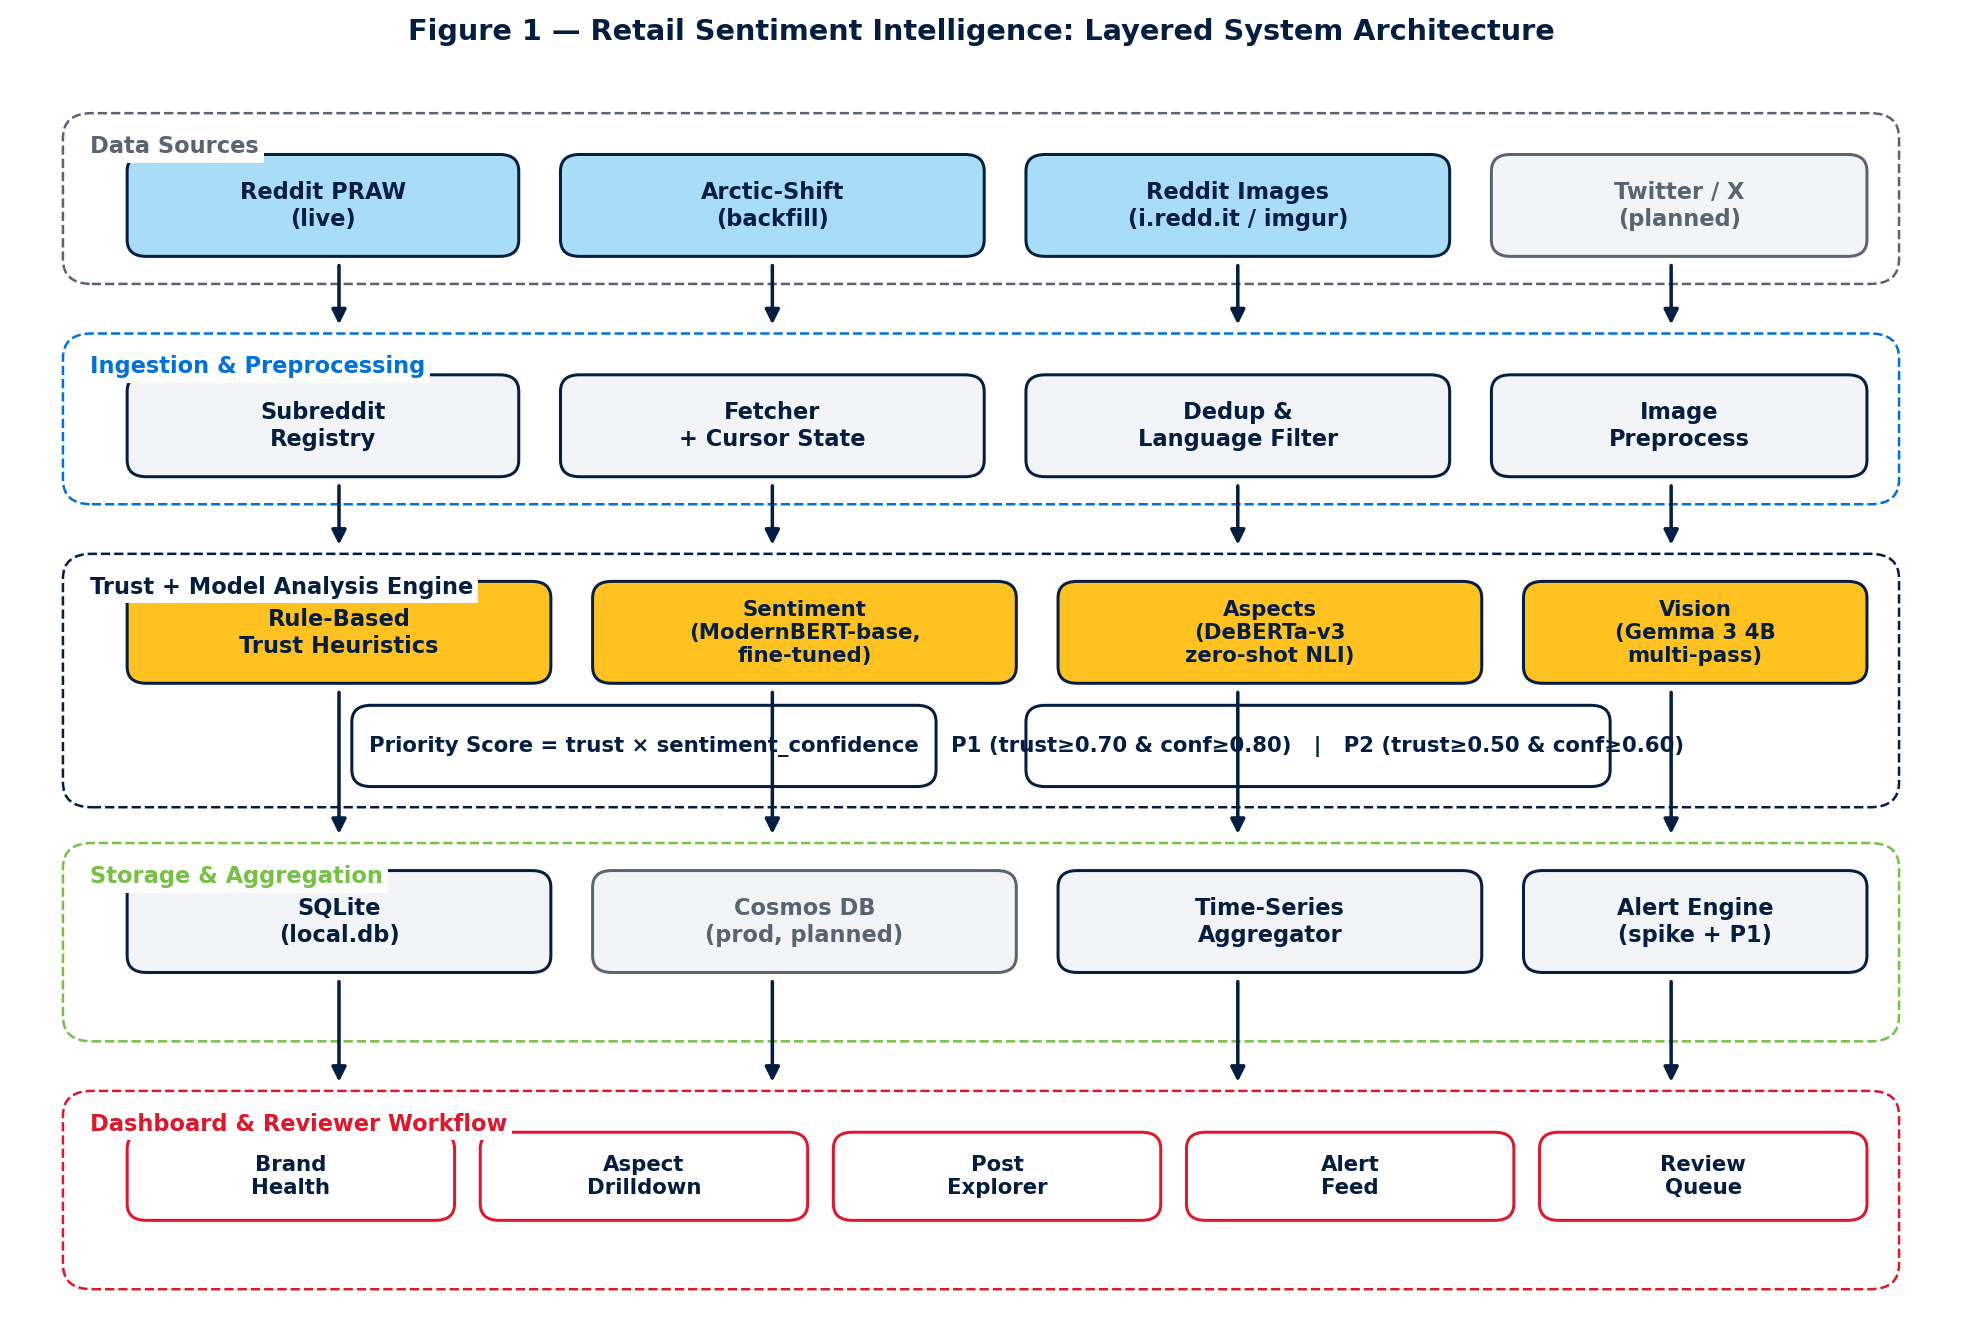
\includegraphics[width=\linewidth]{fig1_architecture}
\caption{Layered System Architecture --- ingestion, storage, AI engine,
aggregation, dashboard, and HITL feedback loop.}
\label{fig:arch}
\end{figure}

\section{End-to-End Pipeline Flow}\label{sec:e2e}
Figure~\ref{fig:pipeline} depicts one post's journey.  A new Reddit RSS entry
is deduplicated by \texttt{post\_id}, passed through the trust scorer, then
routed in parallel through sentiment, aspect, and (if it has an image)
vision.  Results are stored, aggregated into daily brand-health metrics, and
alerts are raised for trust-weighted P1/P2 negatives.  Analysts review the
alert, edit the labels if needed, choose a reply draft, and (optionally) mark
the post as resolved on the Kanban board.  Every analyst action is captured
as a training signal.

\begin{figure}[htbp]
\centering
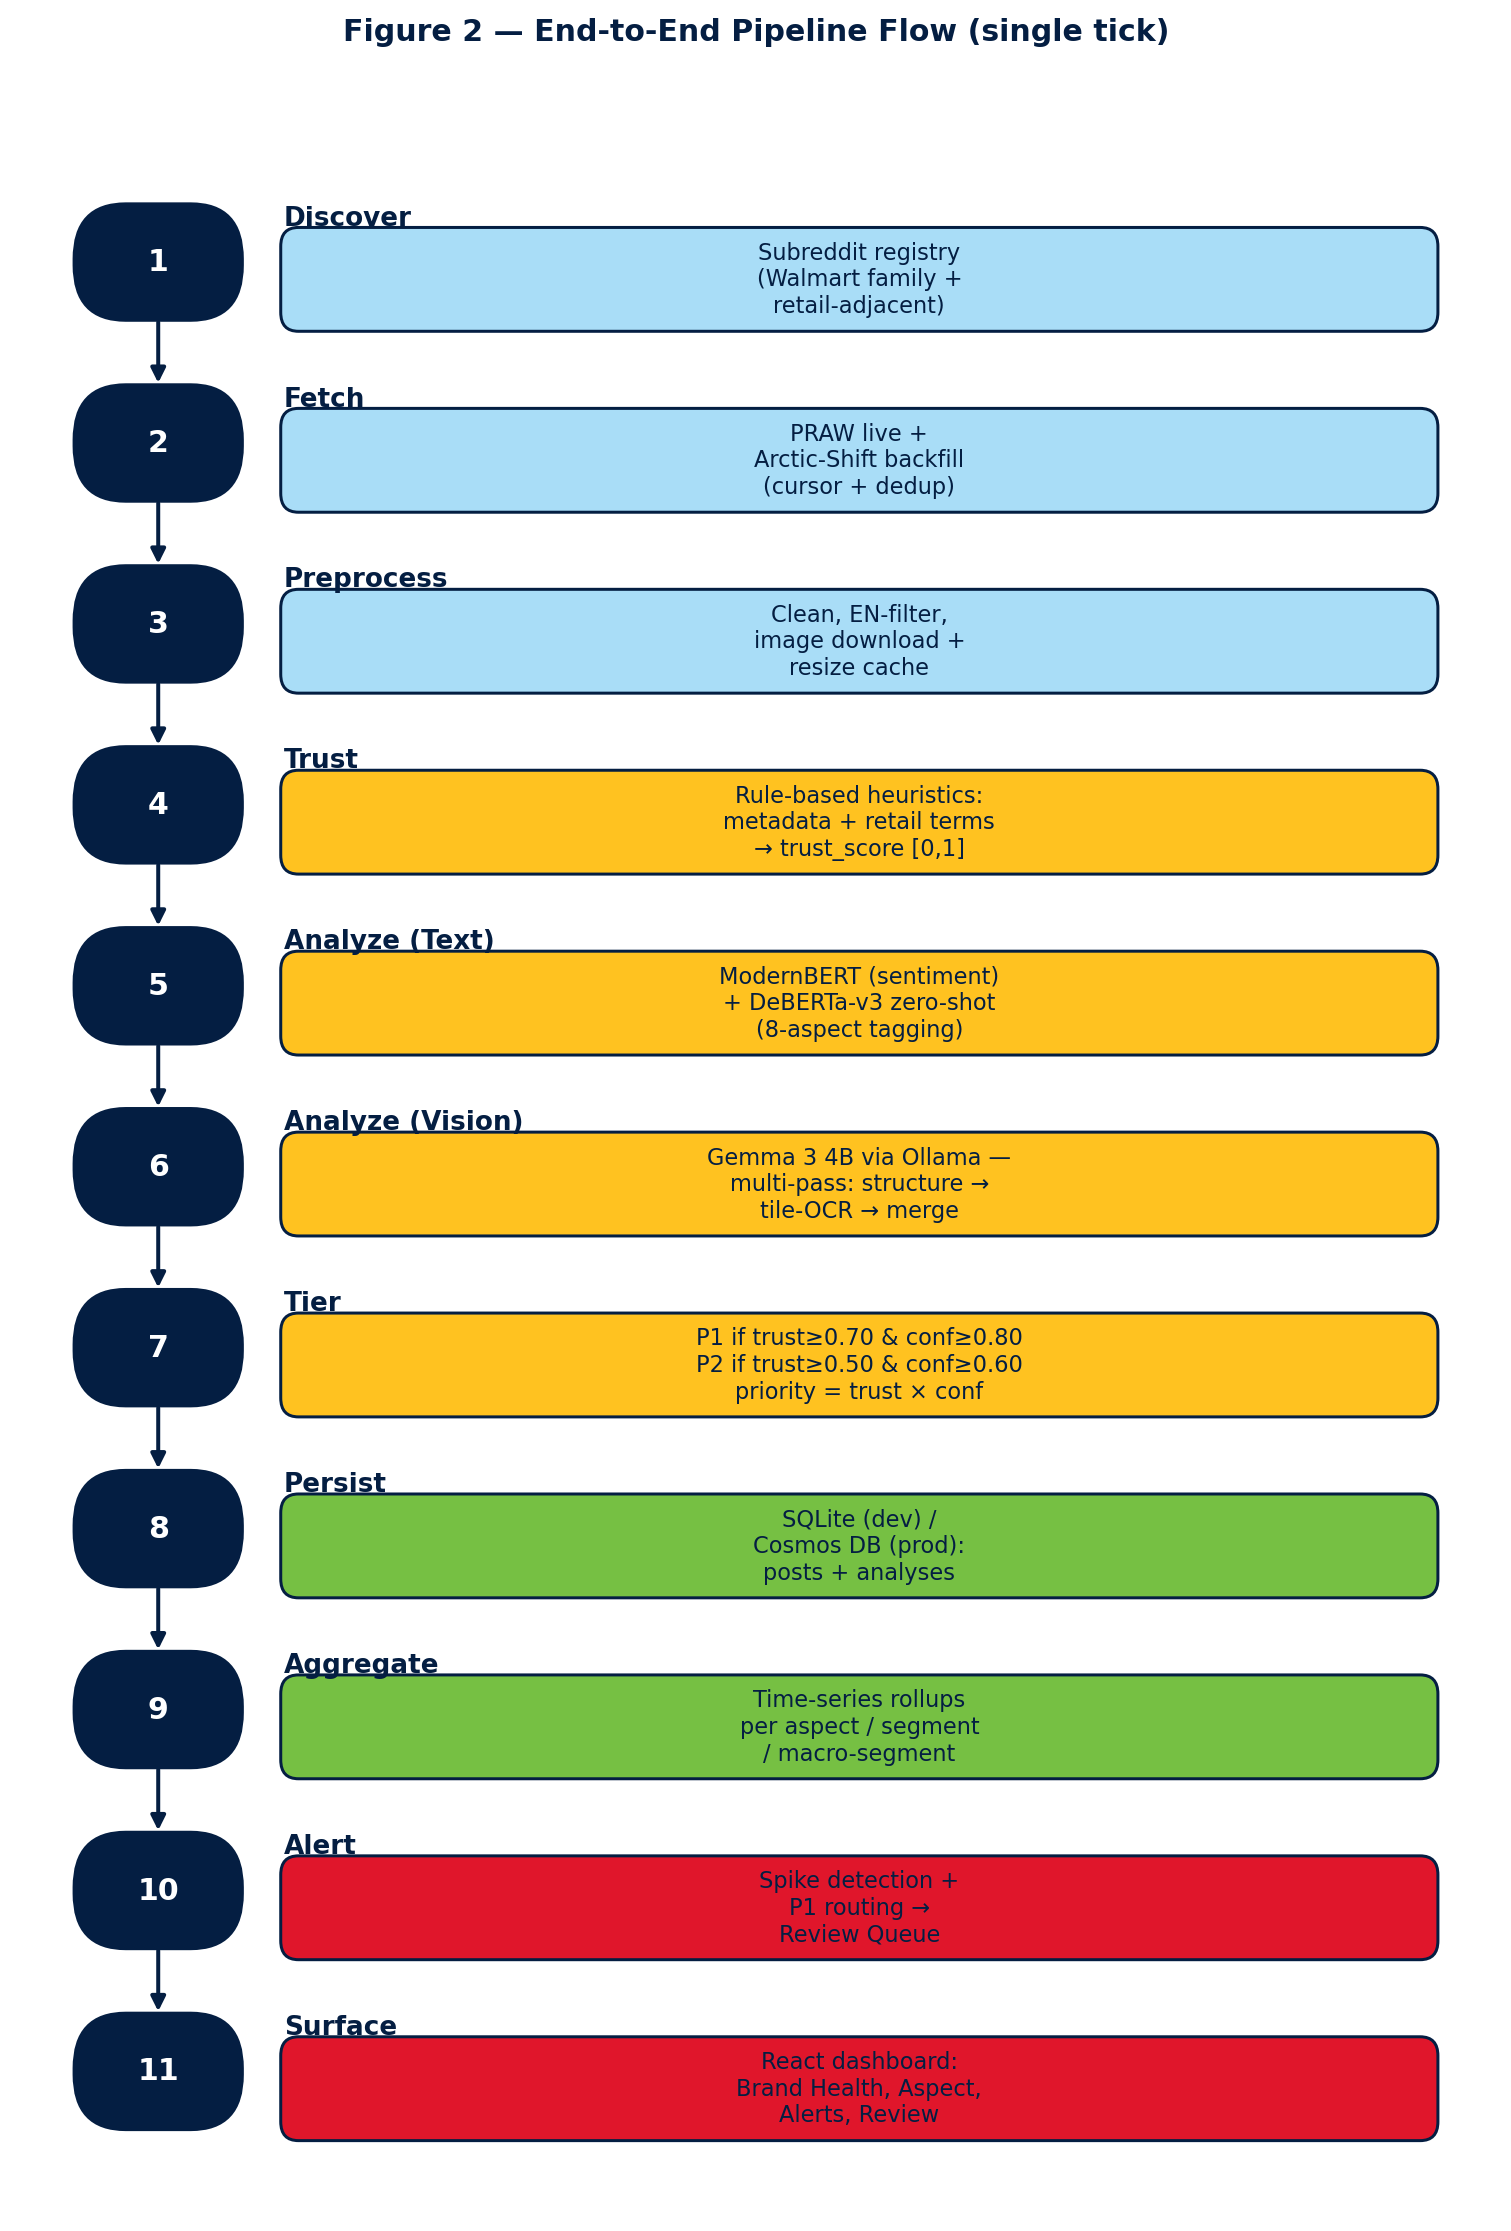
\includegraphics[width=\linewidth]{fig2_pipeline_flow}
\caption{End-to-End Pipeline Flow --- ingestion $\to$ trust $\to$ AI engine
$\to$ aggregation $\to$ alerts $\to$ dashboard $\to$ analyst action $\to$
feedback loop.}
\label{fig:pipeline}
\end{figure}

\chapter{Implementation}\label{ch:impl}

This chapter walks through the running system module by module.  Each section
pairs a short code excerpt from the production source tree with the
corresponding piece of the running dashboard, so the reader can trace an idea
from mathematics to Python to a rendered UI.  All listings are verbatim
extracts from files under \texttt{src/}; comments and blank lines were
trimmed only where they carried no explanatory value.

\section{Data Ingestion and Pre-processing}\label{sec:ingest}
Ingestion runs on a scheduler that polls each subreddit's public RSS feed at
a configurable cadence (default: hourly).  Historical dumps are pulled from
the Arctic Shift API for the sentiment gold set.  Each incoming post is
normalised (HTML-stripped, lowercased for lexical filters), deduplicated by
\texttt{post\_id}, and screenshots are downloaded to a local image cache.
Listing~\ref{lst:arctic} shows the paged fetch loop that drives the
historical pull; it uses \texttt{curl} as transport to sidestep TLS
quirks on corporate networks and emits an \texttt{on\_page} progress
callback so the dashboard's Pipeline view can render live counters.
Figure~\ref{fig:ingest} shows the overall flow.

\begin{lstlisting}[caption={Paged Reddit ingestion with cursor-based dedup ({\tt src/ingestion/arctic\_shift.py}).},label={lst:arctic}]
def fetch_posts_arctic(subreddit, since_utc=0.0, limit=500,
                       self_posts_only=False, on_page=None):
    fetched, before = 0, None
    while fetched < limit:
        batch_size = min(100, limit - fetched)
        params = {"subreddit": subreddit,
                  "limit": str(batch_size), "sort": "desc"}
        if since_utc > 0:  params["after"]  = str(int(since_utc))
        if before:         params["before"] = str(int(before))
        if self_posts_only: params["is_self"] = "true"

        data = _curl_get(f"{BASE_URL}?{urlencode(params)}")
        if not data or not (posts := data.get("data", [])):
            break

        for post in posts:
            created = post.get("created_utc", 0)
            if since_utc > 0 and created <= since_utc:
                continue                     # already ingested
            selftext = (post.get("selftext") or "").lower()
            if selftext in ("[deleted]", "[removed]"):
                continue                     # moderator-scrubbed
            if (norm := _normalize_post(post, subreddit)):
                yield norm
                fetched += 1

        if len(posts) < batch_size: break
        before = posts[-1].get("created_utc", 0)  # page cursor
        time.sleep(0.5)                            # be polite
\end{lstlisting}

\begin{figure}[htbp]
\centering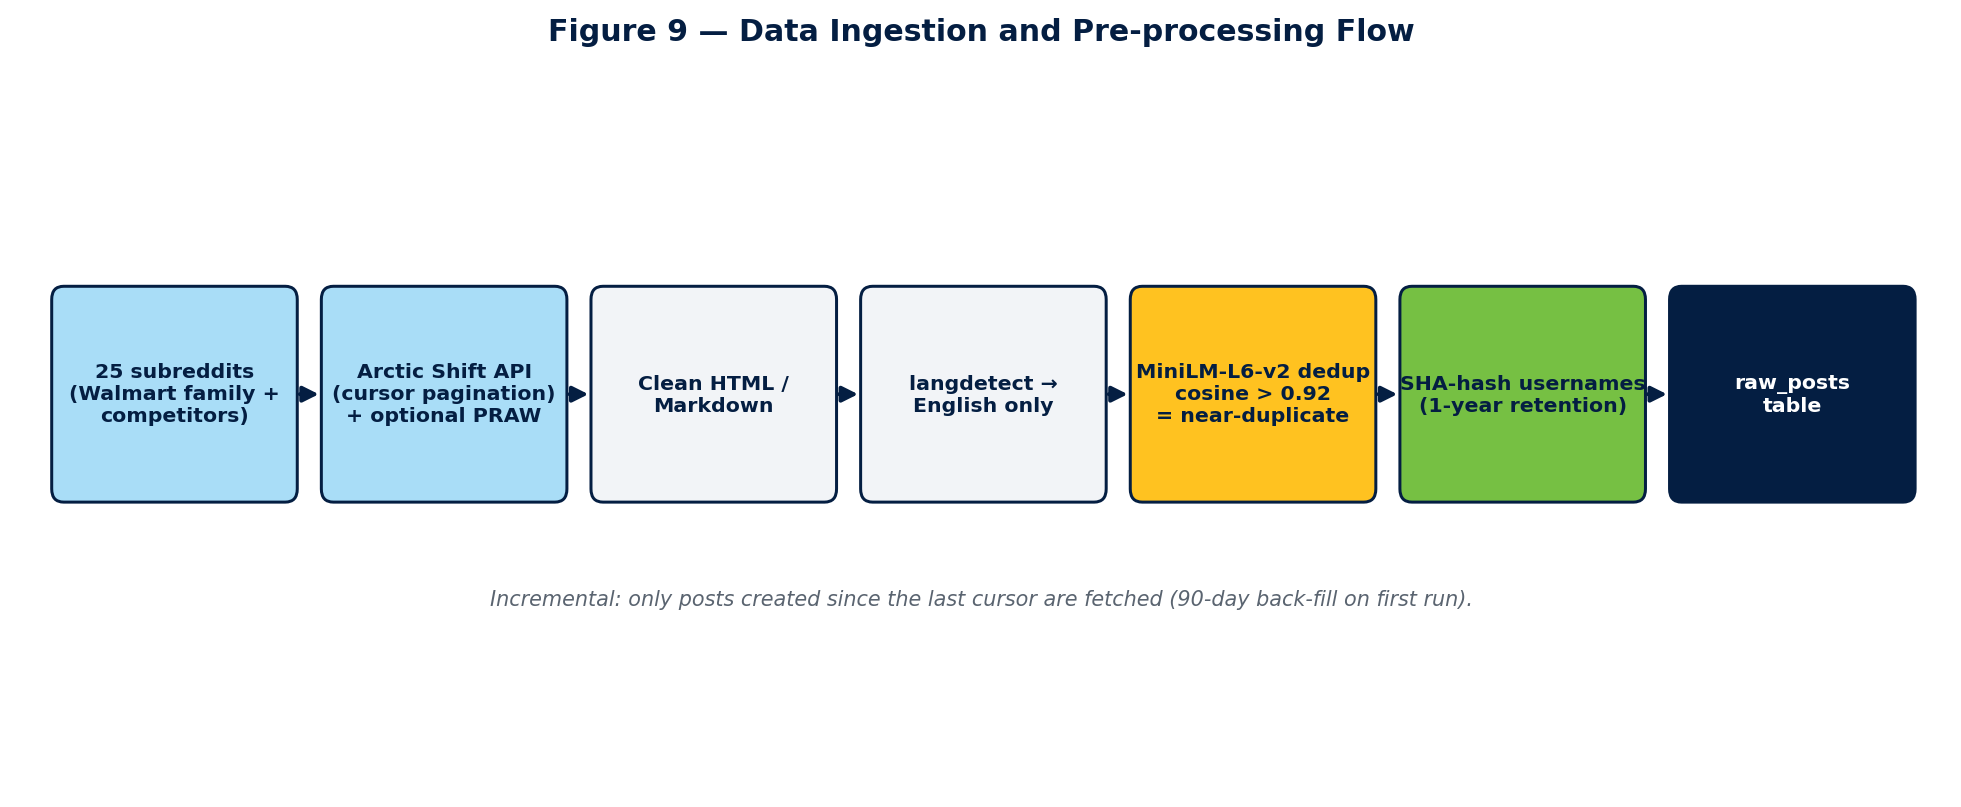
\includegraphics[width=\linewidth]{fig9_ingestion_flow}
\caption{Data ingestion and pre-processing flow.}\label{fig:ingest}
\end{figure}

\section{Trust-Score Module}\label{sec:trust}
The trust score $T \in [0,1]$ blends account metadata and content signals:
$T = 0.4\,M + 0.3\,C + 0.3\,L$ where $M$ is a metadata score
(account\_age, karma, verified\_email, cakeday), $C$ is an LLM-graded
credibility signal, and $L$ is a lexical retail-insider score.  Priority
tiers are: P1 iff $T \ge 0.75$ and sentiment is negative with confidence
$\ge 0.75$; P2 iff $T \ge 0.55$ and negative with confidence $\ge 0.65$.
The core scorer is small on purpose --- Listing~\ref{lst:trust} shows the
entire \texttt{TrustScorer.score()} method.  It also implements the
cost-shaping heuristic that only invokes the LLM credibility check when
metadata is genuinely ambiguous ($0.3 < M < 0.8$); outside that band
metadata is already decisive.  Figure~\ref{fig:trust} depicts the
composition.  Every constant is exposed in the dashboard so that a
stakeholder can argue with the rule rather than guess at a black box.

\begin{lstlisting}[caption={Combined trust scorer with cost-shaped LLM invocation ({\tt src/trust/scorer.py}).},label={lst:trust}]
def score(self, unit: dict) -> dict:
    meta  = score_metadata(unit, self.config)     # M
    dedup = score_originality(unit)               # L

    # LLM credibility (C) --- only when metadata is ambiguous.
    # Outside the band, metadata is decisive, so we skip the call
    # to cap cost on cloud providers.
    llm_score, llm_flags = 0.5, []
    if self.llm_client and 0.3 < meta < 0.8:
        r = self.llm_client.check_credibility(
            text=self._get_text(unit),
            metadata=unit.get("author_metadata", {}))
        llm_score = r.get("credibility_score", 0.5)
        llm_flags = r.get("flags", [])

    # T = 0.4 M + 0.3 dedup + 0.3 LLM, clamped to [0, 1]
    combined = (self.config.weight_metadata * meta   +
                self.config.weight_dedup    * dedup  +
                self.config.weight_llm      * llm_score)
    combined = round(min(max(combined, 0.0), 1.0), 3)

    unit["trust_score"]      = combined
    unit["trust_components"] = {"metadata": meta,
                                "dedup":    dedup,
                                "llm":      llm_score}
    unit["trust_flags"]      = llm_flags
    unit["is_trusted"]       = combined >= self.config.threshold
    if not unit["is_trusted"]:
        unit["processing_status"] = "flagged_low_trust"
    return unit
\end{lstlisting}

\begin{figure}[htbp]
\centering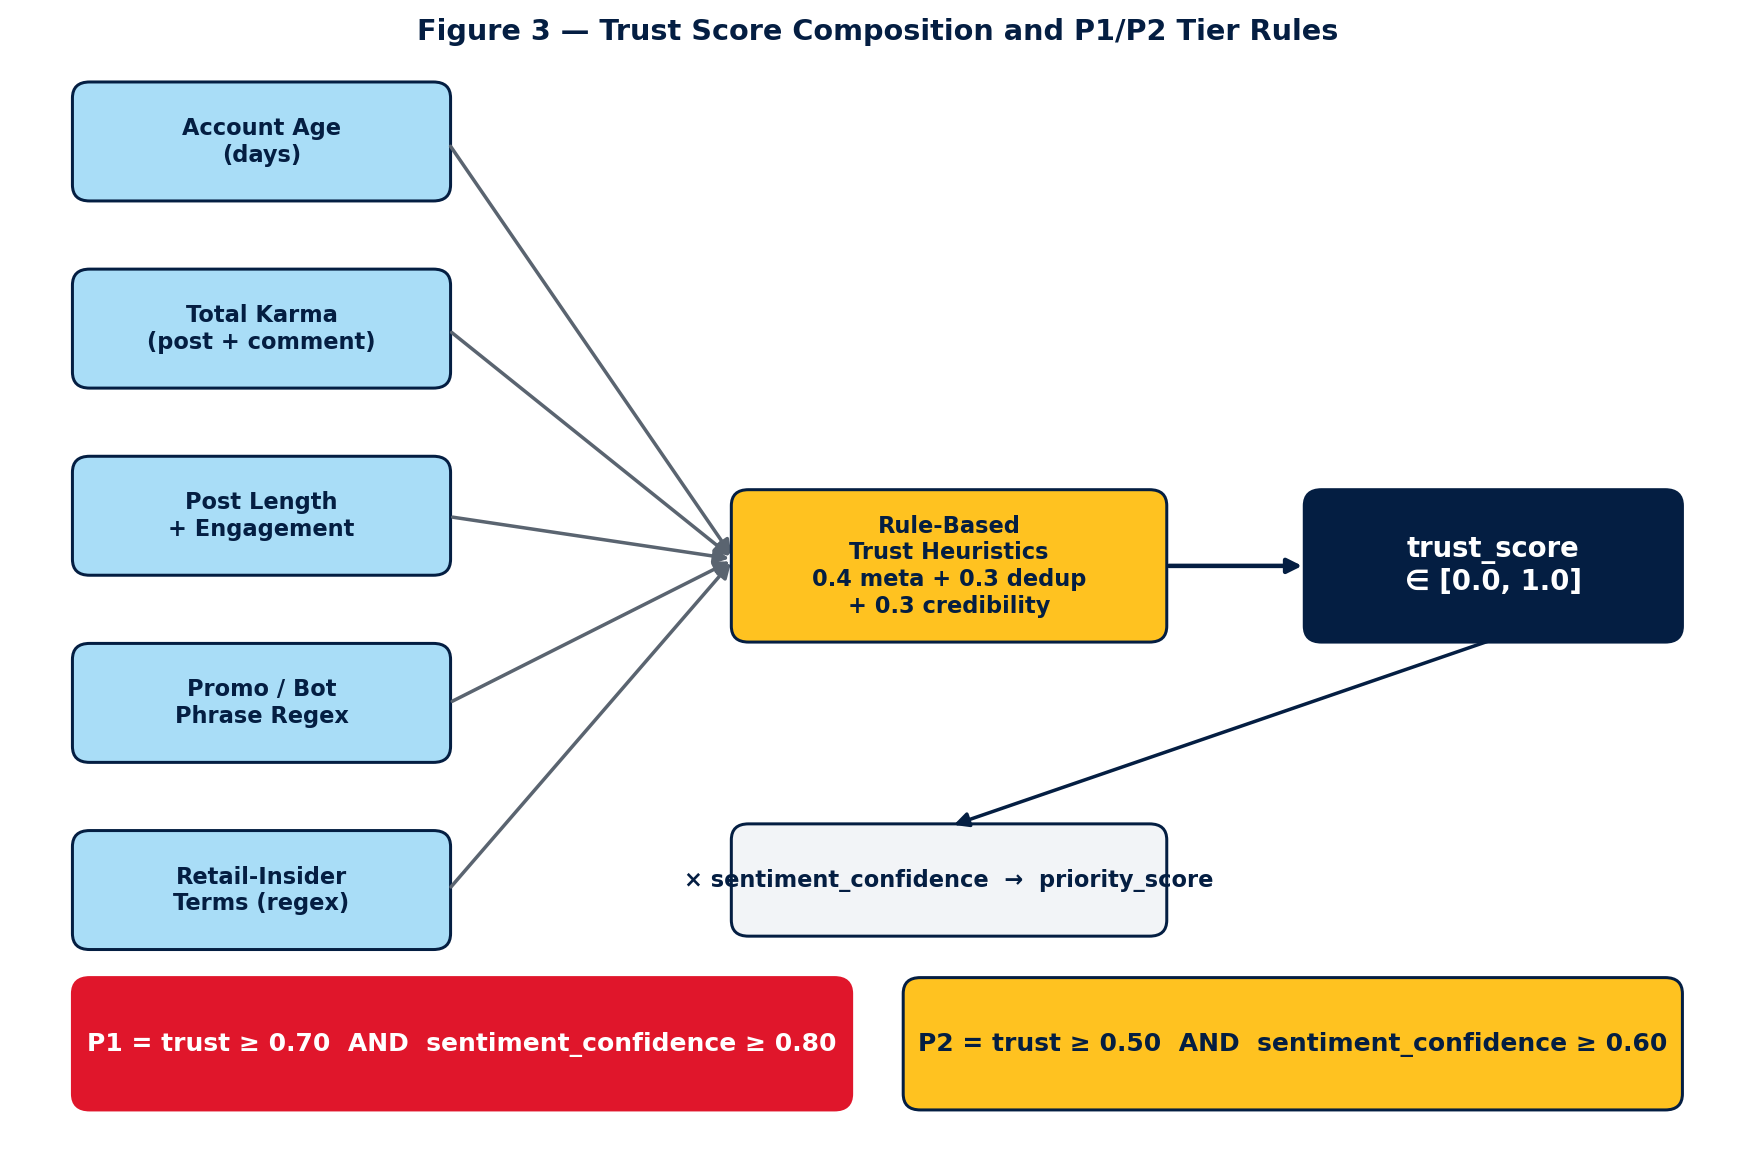
\includegraphics[width=\linewidth]{fig3_trust_composition}
\caption{Trust-Score composition and P1/P2 tier rules.}\label{fig:trust}
\end{figure}

\section{Sentiment Classification (ModernBERT)}\label{sec:sent}
The sentiment head is a fine-tuned ModernBERT-base with a three-class
softmax (positive, neutral, negative).  Training used a three-stage
curriculum: (Stage 1) 8k pseudo-labelled tweets from the twitter-roberta
teacher, (Stage 2) 2k retail-focused Reddit posts pseudo-labelled by the
same teacher, and (Stage 3) 200 hand-labelled retail Reddit posts for a
final domain adaptation.  See Figure~\ref{fig:curriculum}.  The 5-fold
out-of-fold macro-F1 rose from the baseline of 0.6272 to \textbf{0.7642};
long-post accuracy (bucket $\ge 512$~tokens, $n{=}7$, all negative-class)
rose from 5/7 correct on the RoBERTa baseline to \textbf{7/7 correct}
on ModernBERT.

At inference time the sentiment head is wrapped by a thin
\texttt{SentimentAnalyzer} that owns exactly two responsibilities: assemble
the prompt string (subreddit-aware, and injecting an
\texttt{[image: \dots]} tail when a Gemma caption is present), and shape
the model's output into the analysis record the storage layer expects.
Listing~\ref{lst:analyzer} shows both.

\begin{lstlisting}[caption={Sentiment orchestration with vision-caption fusion ({\tt src/analysis/analyzer.py}).},label={lst:analyzer}]
def _get_text(self, unit: dict) -> str:
    """Compose a subreddit-tagged prompt; append the Gemma caption
    as [image: ...] so downstream models see it as post body."""
    title = unit.get("title", "") or ""
    body  = unit.get("body",  "") or ""
    sub   = unit.get("subreddit", "unknown")
    cap   = (unit.get("image_caption") or "").strip()
    cap_suffix = f" [image: {cap}]" if cap else ""

    if unit.get("unit_type") == "comment":
        return f'Comment from r/{sub}: "{body}"'
    if title and body:
        return f'Post from r/{sub}: "{title}" -- {body}{cap_suffix}'
    if title:
        return f'Post from r/{sub}: "{title}"{cap_suffix}'
    if body:
        return f'Post from r/{sub}: "{body}{cap_suffix}"'
    # Image-only post: the caption IS the content.
    return f'Post from r/{sub}: "{cap}"' if cap else f'Post from r/{sub}: ""'

def _build_analysis_record(self, unit, result):
    unit_id = unit.get("id", "")
    conf    = result.get("sentiment_confidence", 0.0)
    return {
        "id": f"analysis_{unit_id}",  "post_id": unit_id,
        "subreddit":            unit.get("subreddit", ""),
        "trust_score":          unit.get("trust_score"),
        "sentiment":            result.get("sentiment", "neutral"),
        "sentiment_confidence": conf,
        "aspects":              result.get("aspects", []),
        "key_phrases":          result.get("key_phrases", []),
        "summary":              result.get("summary", ""),
        "model_used":     result.get("model_used", self.llm.model_name),
        "model_version":  result.get("model_version", self.llm.model_version),
        "analyzed_at":    datetime.now(timezone.utc).isoformat(),
        "needs_review":   conf < self.config.confidence_threshold,
        "partition_key":  unit.get("subreddit", ""),
    }
\end{lstlisting}

\begin{figure}[htbp]
\centering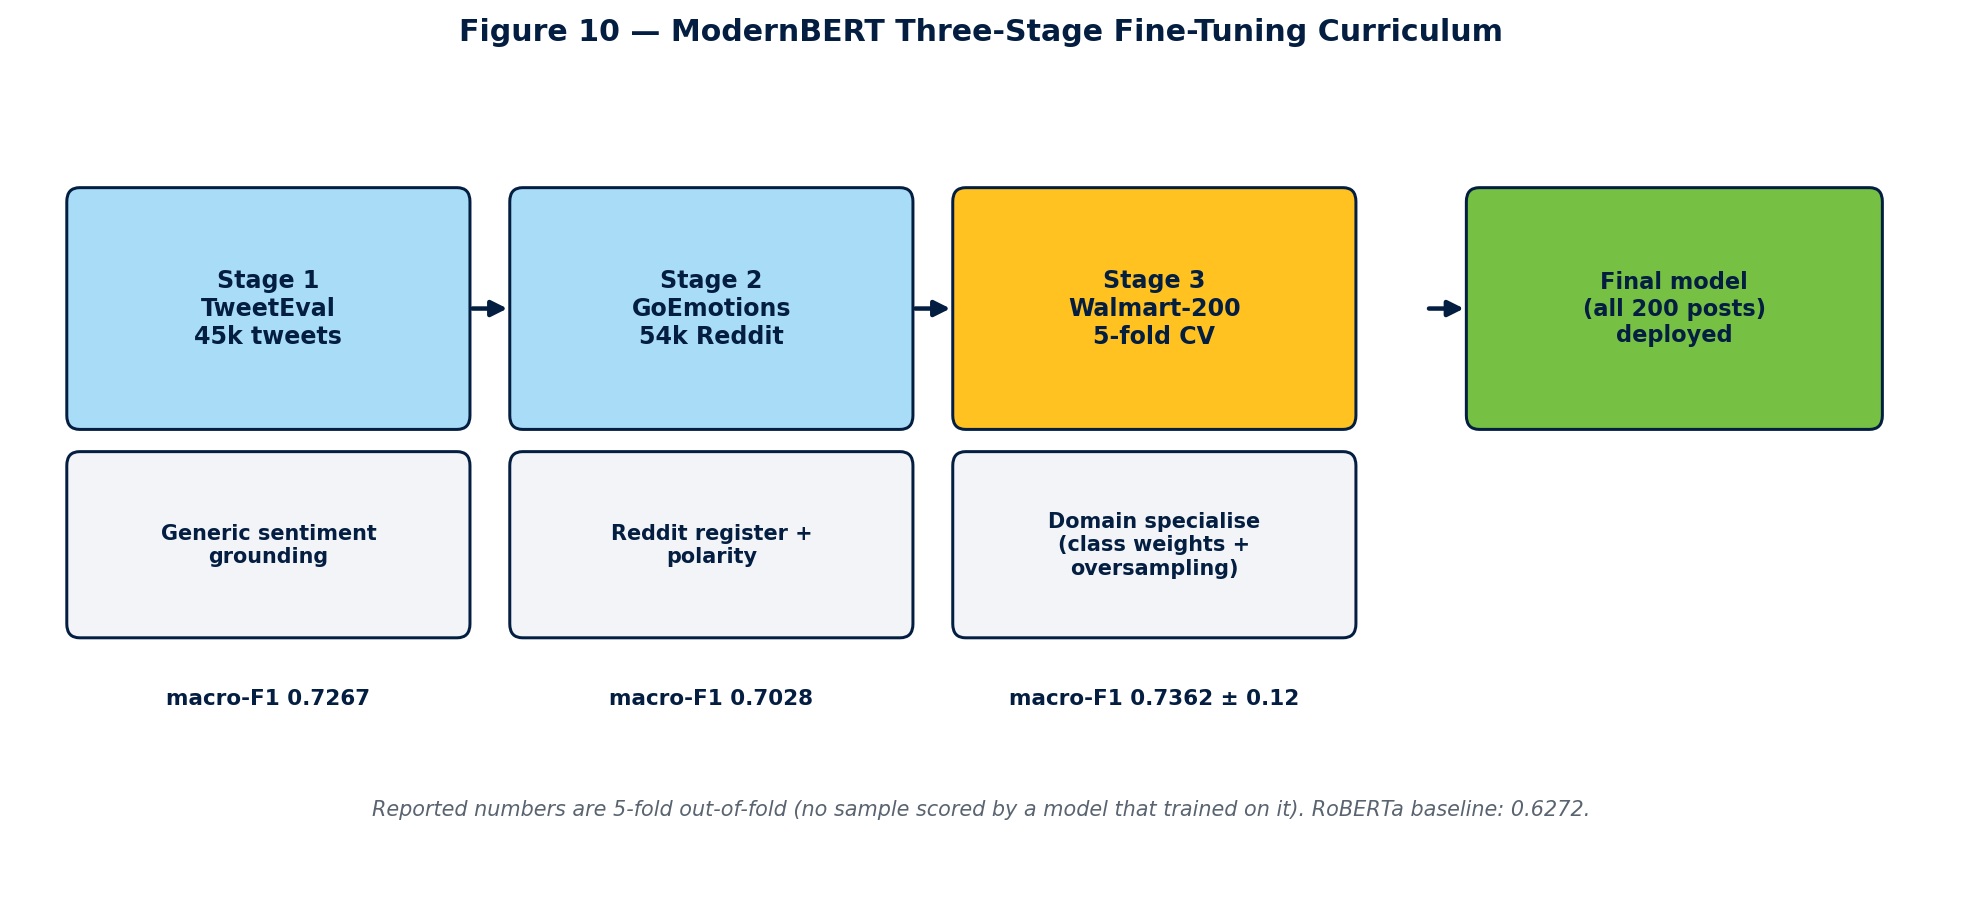
\includegraphics[width=\linewidth]{fig10_modernbert_curriculum}
\caption{ModernBERT three-stage fine-tuning curriculum.}\label{fig:curriculum}
\end{figure}

\section{Aspect-Based Opinion Mining}\label{sec:aspect}
Aspects are extracted with a zero-shot NLI classifier
(\texttt{mDeBERTa-v3-base-xnli-multilingual-nli-2mil7}) scored against a fixed
eight-aspect taxonomy (Table~\ref{tab:aspects}).  A post can carry multiple
aspects when their entailment scores are above threshold~0.55.
Figure~\ref{fig:aspect} illustrates the NLI framing.  On cloud LLM
providers the same taxonomy is enforced with the structured JSON prompt in
Listing~\ref{lst:aspect-prompt}: the model is told exactly which aspect
group applies to which subreddit (customer vs.\ employee), which prevents
the ``rude cashier'' $\leftrightarrow$ ``bad manager'' bleed that
plagued the first-cut prompts.

\begin{lstlisting}[caption={Aspect taxonomy enforced in the JSON-mode system prompt ({\tt src/analysis/prompts.py}).},label={lst:aspect-prompt}]
SENTIMENT_ASPECT_SYSTEM_PROMPT = """You are a retail analyst ...

Rules:
1. Sentiment must be one of: "positive", "negative", "neutral".
2. Choose aspects from the correct group based on the subreddit:

   CUSTOMER aspects (r/walmart, r/samsclub, r/WalmartPlus, ...):
     store_experience, online_app, delivery_pickup, product_quality,
     returns, customer_support, pricing

   EMPLOYEE aspects (r/WalmartEmployees, r/OGPBackroom,
                     r/Sparkdriver, r/walmart_RX, ...):
     workforce_hr, pay_benefits, management, safety_policy, workload

3. A post can have 0 aspects (off-topic) or multiple aspects.
4. NEVER mix customer and employee aspects in the same post.
5. Handle sarcasm and slang (Reddit tone). "Love how my order
   arrived 3 days late" = negative + delivery_pickup.
6. Confidence scores (0.0-1.0) for each prediction.

Output JSON:
{
  "sentiment": "positive|negative|neutral",
  "sentiment_confidence": 0.0-1.0,
  "aspects": [
    {"aspect": "<name>", "sentiment": "...", "confidence": 0.0-1.0}
  ],
  "key_phrases": ["phrase1", "phrase2"],
  "summary": "One sentence summary of the issue/praise"
}"""
\end{lstlisting}

\begin{table}[htbp]\centering
\caption{Eight-aspect retail taxonomy.}\label{tab:aspects}
\small
\begin{tabular}{@{}ll@{}}\toprule
\bfseries Aspect & \bfseries Example indicative terms\\\midrule
Pricing               & ``\$2 more this week'', ``price hike'', ``clearance''\\
Product quality       & ``broken'', ``expired'', ``mouldy''\\
Customer service      & ``rude cashier'', ``no help'', ``manager''\\
Store experience      & ``dirty floor'', ``long line'', ``restroom''\\
Online / app          & ``app crash'', ``payment failed'', ``2FA loop''\\
Delivery / pickup     & ``missed slot'', ``OGP'', ``Spark driver''\\
Returns               & ``refused return'', ``restocking fee''\\
Account / login       & ``locked out'', ``password reset''\\\bottomrule
\end{tabular}
\end{table}

\begin{figure}[htbp]
\centering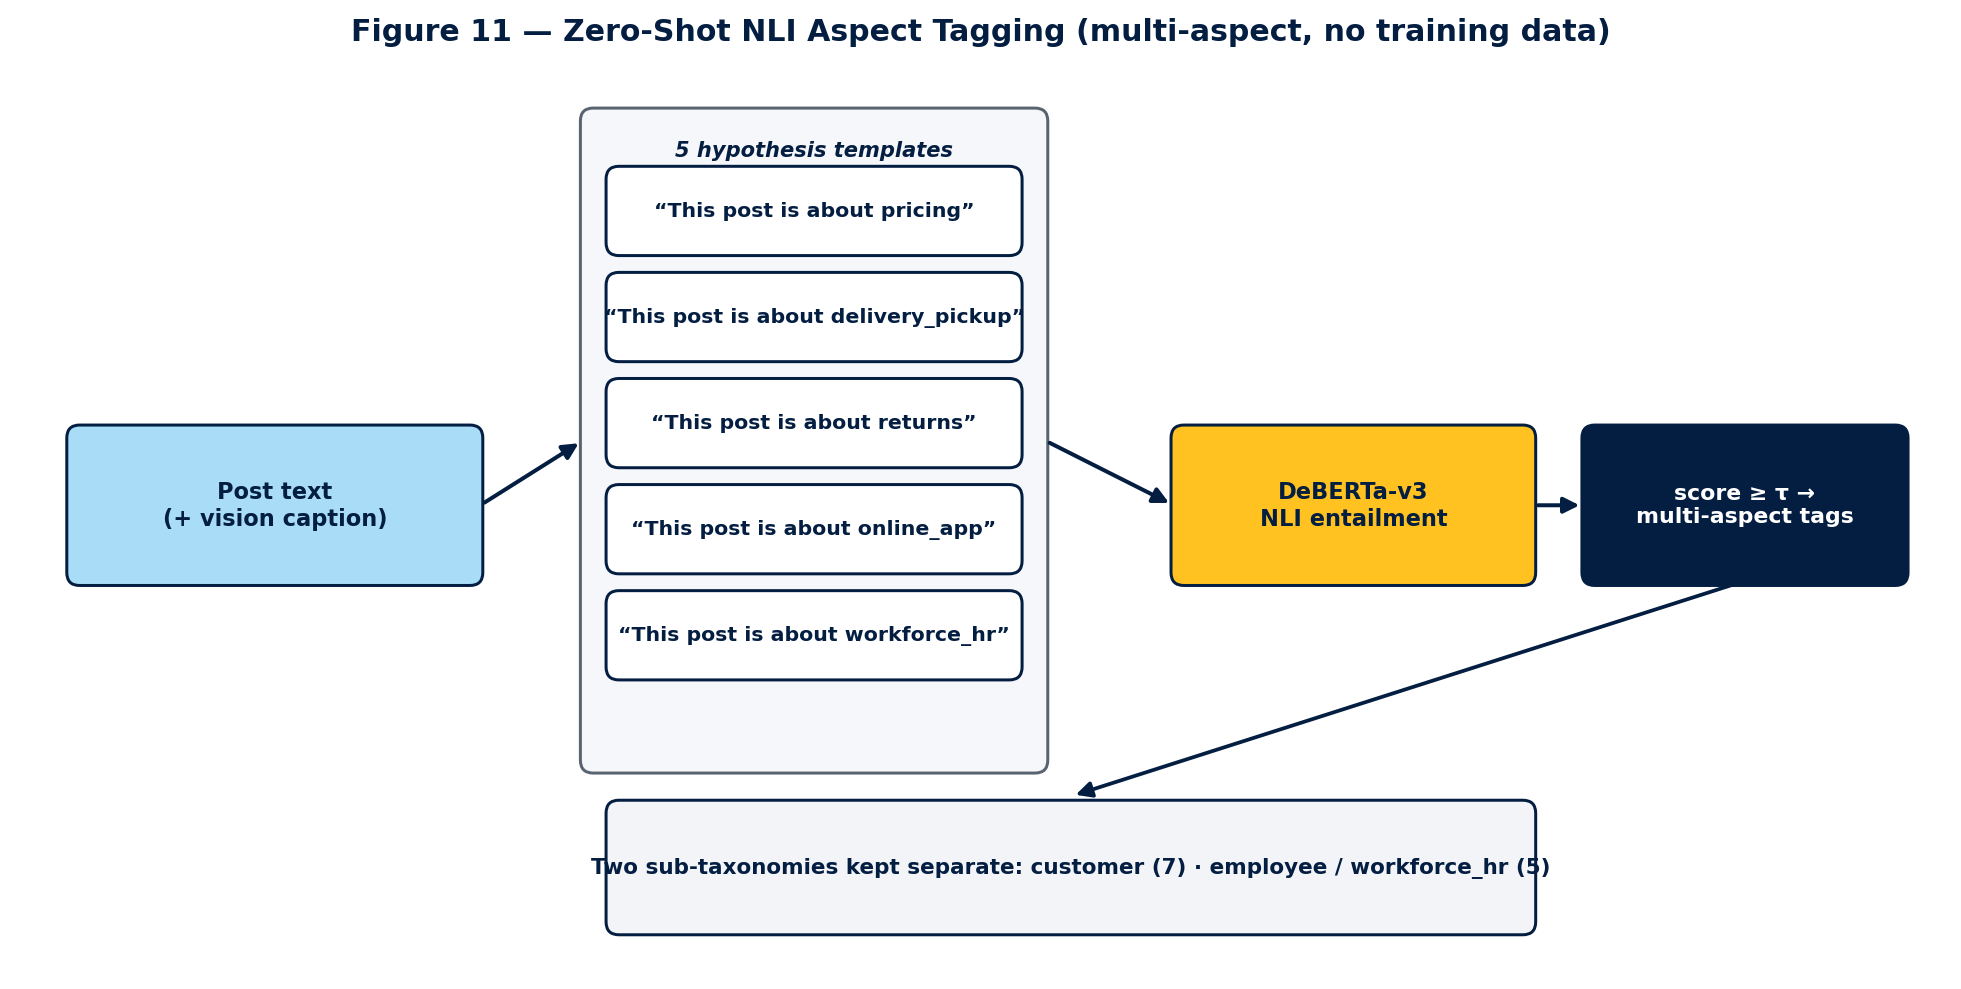
\includegraphics[width=0.95\linewidth]{fig11_aspect_nli}
\caption{Zero-shot NLI aspect tagging.}\label{fig:aspect}
\end{figure}

\section{Vision / Image Processing}\label{sec:vision}
Screenshots are captioned by Gemma~3 4B via Ollama using a multi-pass prompt
pipeline: Pass~1 identifies the image \emph{structure}
(screenshot / receipt / product page / error dialog / meme / photo);
Pass~2 tiles the image at native resolution and extracts text per tile;
Pass~3 merges the tile texts against the structure into 2--4 factual
sentences with a strict ``do not invent'' clause.  A circuit breaker
disables the whole vision branch after three consecutive Ollama failures
so a stopped daemon cannot flood the logs.
Figure~\ref{fig:vision} shows the pipeline.  Hallucination rate on 32
retail screenshots dropped from 50\% (single pass) to \textbf{0\%}; text
extraction rose from 25\% to \textbf{75\%}.
Listing~\ref{lst:vision} shows the entry point and the merge prompt that
carries the anti-hallucination clause.

\begin{lstlisting}[caption={Vision multi-pass caption entry point and merge prompt ({\tt src/analysis/vision.py}).},label={lst:vision}]
MERGE_PROMPT = """Combine these observations about a Walmart-related
image into 2-4 clear sentences.

Image type: {structure}
Text found in different regions:
{tile_texts}

Write a factual description that captures: what type of
screen/image this is, all important text (especially errors,
prices, status messages), and what the customer might be
complaining about. Do NOT invent details not mentioned above."""

def caption_enhanced(self, image_path: Path) -> str:
    if not self.cfg.enabled or not Path(image_path).exists():
        return ""
    img = Image.open(image_path)

    # Pass 1: structure identification
    full_b64  = self._image_to_b64(img)
    structure = self._call_ollama(self.model, STRUCTURE_PROMPT, full_b64)
    if not structure:
        return self.caption(image_path)           # fall back

    # Only tile screenshots / receipts / app screens; photos and
    # memes are fine as single-pass.
    if not any(kw in structure.lower() for kw in
               ("screenshot","receipt","app_screen",
                "error_dialog","document","product_page")):
        return self.caption(image_path)

    # Pass 2 + 3: tile at native resolution and extract text per tile
    tiles, tile_texts = self._create_tiles(img), []
    for i, b64 in enumerate(tiles):
        t = self._call_ollama(self.model, TILE_TEXT_PROMPT, b64)
        if t and "NO TEXT" not in t.upper():
            tile_texts.append(f"Region {i+1}: {t}")

    merged = self._call_ollama(
        self.model,
        MERGE_PROMPT.format(structure=structure,
                            tile_texts="\n".join(tile_texts)),
        full_b64)
    return merged or self.caption(image_path)
\end{lstlisting}

\begin{figure}[htbp]
\centering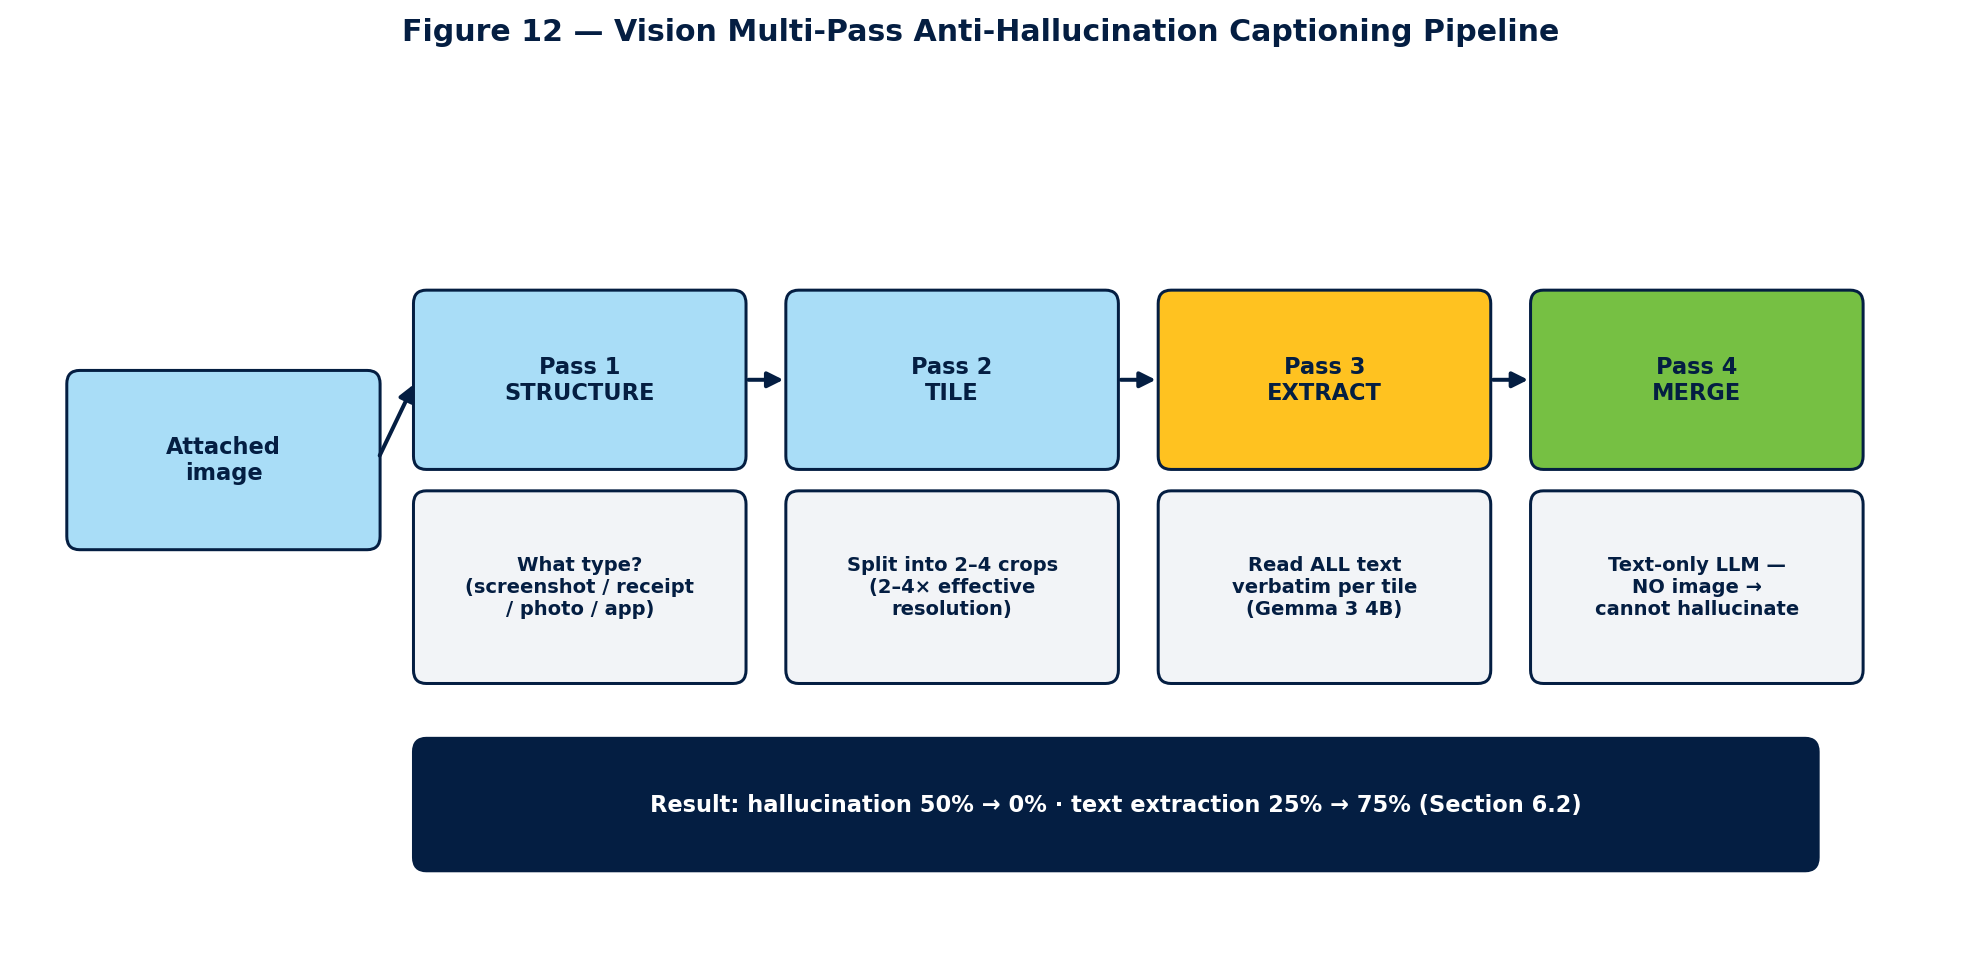
\includegraphics[width=\linewidth]{fig12_vision_multipass}
\caption{Vision multi-pass anti-hallucination pipeline.}\label{fig:vision}
\end{figure}

\section{Aggregation, Alerts and Notifications}\label{sec:agg}
The aggregator writes daily brand-health rollups (sentiment share, top
aspects, trust bucket) into SQLite.  The alert engine fires on volume,
sentiment-crash, emerging-topic and competitor rules; each rule reads its
thresholds from \texttt{data/alert\_rules.json}, which the dashboard's
Alert Rules panel writes to.  Listing~\ref{lst:alerts} shows the two
detectors that drive the majority of P1/P2 traffic: a volume-spike detector
that fires when today's post count crosses $\mu + \sigma\!\cdot\!\theta$ of
the trailing 7-day mean, and a sentiment-crash detector that fires when
the negative share jumps by more than 0.30 versus yesterday.  Alerts flow
to the dashboard's Alert Feed (\S\ref{sec:dash}) and, optionally, to an
email digest.  Figure~\ref{fig:alerts} shows the routing.

\begin{lstlisting}[caption={Volume-spike and sentiment-crash detectors ({\tt src/alerts/engine.py}).},label={lst:alerts}]
def detect_volume_spike(self, sigma_threshold: float = 2.0):
    """Fire when today's post count is > mu + sigma * threshold of
       the trailing 7-day mean."""
    now   = datetime.now(timezone.utc)
    today = now.strftime("%Y-%m-%d")
    today_agg = self.storage.get_item("aggregates",
                                      f"agg_{today}_daily", today)
    if not today_agg: return []

    counts = []
    for i in range(1, 8):
        d = (now - timedelta(days=i)).strftime("%Y-%m-%d")
        past = self.storage.get_item("aggregates", f"agg_{d}_daily", d)
        if past: counts.append(past.get("total_posts", 0))
    if len(counts) < 3: return []

    mu  = sum(counts) / len(counts)
    std = math.sqrt(sum((x-mu)**2 for x in counts) / len(counts))
    if std == 0: return []

    n = today_agg.get("total_posts", 0)
    z = (n - mu) / std
    if z <= sigma_threshold: return []
    return [{
        "id": f"alert_spike_{today}", "type": "volume_spike",
        "severity": "high" if z > 3.0 else "medium",
        "title": f"Volume spike: {n} posts today "
                 f"({z:.1f}sigma above mean)",
        "details": {"today_count": n, "mean_7d": round(mu, 1),
                    "std_7d":  round(std, 1),
                    "z_score": round(z, 2)},
        "detected_at": now.isoformat(), "time_window": today,
    }]

def detect_sentiment_crash(self, drop_threshold: float = 0.3):
    """Fire when negative share jumps > 0.3 vs yesterday."""
    now   = datetime.now(timezone.utc)
    today = now.strftime("%Y-%m-%d")
    yday  = (now - timedelta(days=1)).strftime("%Y-%m-%d")
    t = self.storage.get_item("aggregates", f"agg_{today}_daily", today)
    y = self.storage.get_item("aggregates", f"agg_{yday}_daily",  yday)
    if not t or not y: return []
    delta = (t.get("sentiment_distribution", {}).get("negative", 0)
           - y.get("sentiment_distribution", {}).get("negative", 0))
    if delta <= drop_threshold: return []
    return [{
        "id": f"alert_crash_{today}", "type": "sentiment_crash",
        "severity": "critical" if delta > 0.4 else "high",
        "title": f"Sentiment crash: negative +{delta:.0%} vs yesterday",
        "details": {"delta": round(delta, 3)},
        "detected_at": now.isoformat(), "time_window": today,
    }]
\end{lstlisting}

\begin{figure}[htbp]
\centering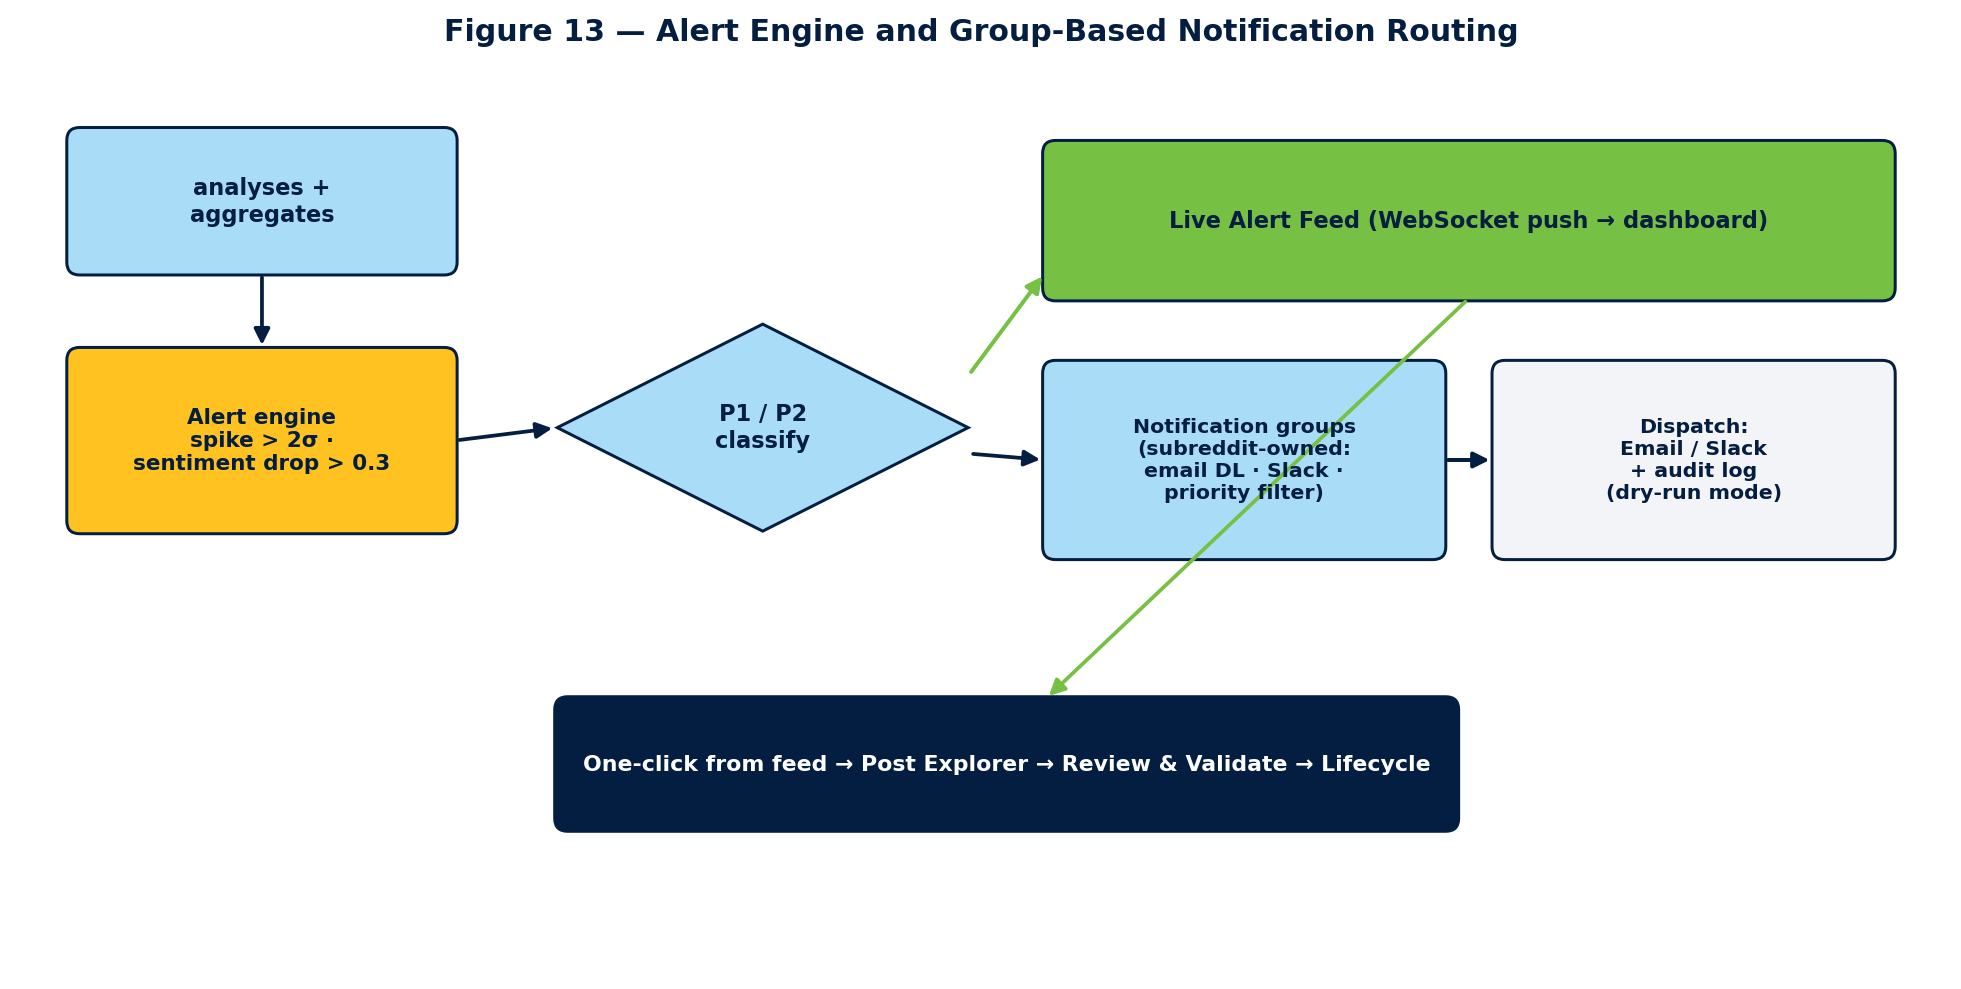
\includegraphics[width=\linewidth]{fig13_alert_routing}
\caption{Alert engine and notification routing.}\label{fig:alerts}
\end{figure}

The rendered Alert Feed is shown in Figure~\ref{fig:ui:alerts}; each row
is one entry from the JSON returned by the detectors above.

\begin{figure}[htbp]
\centering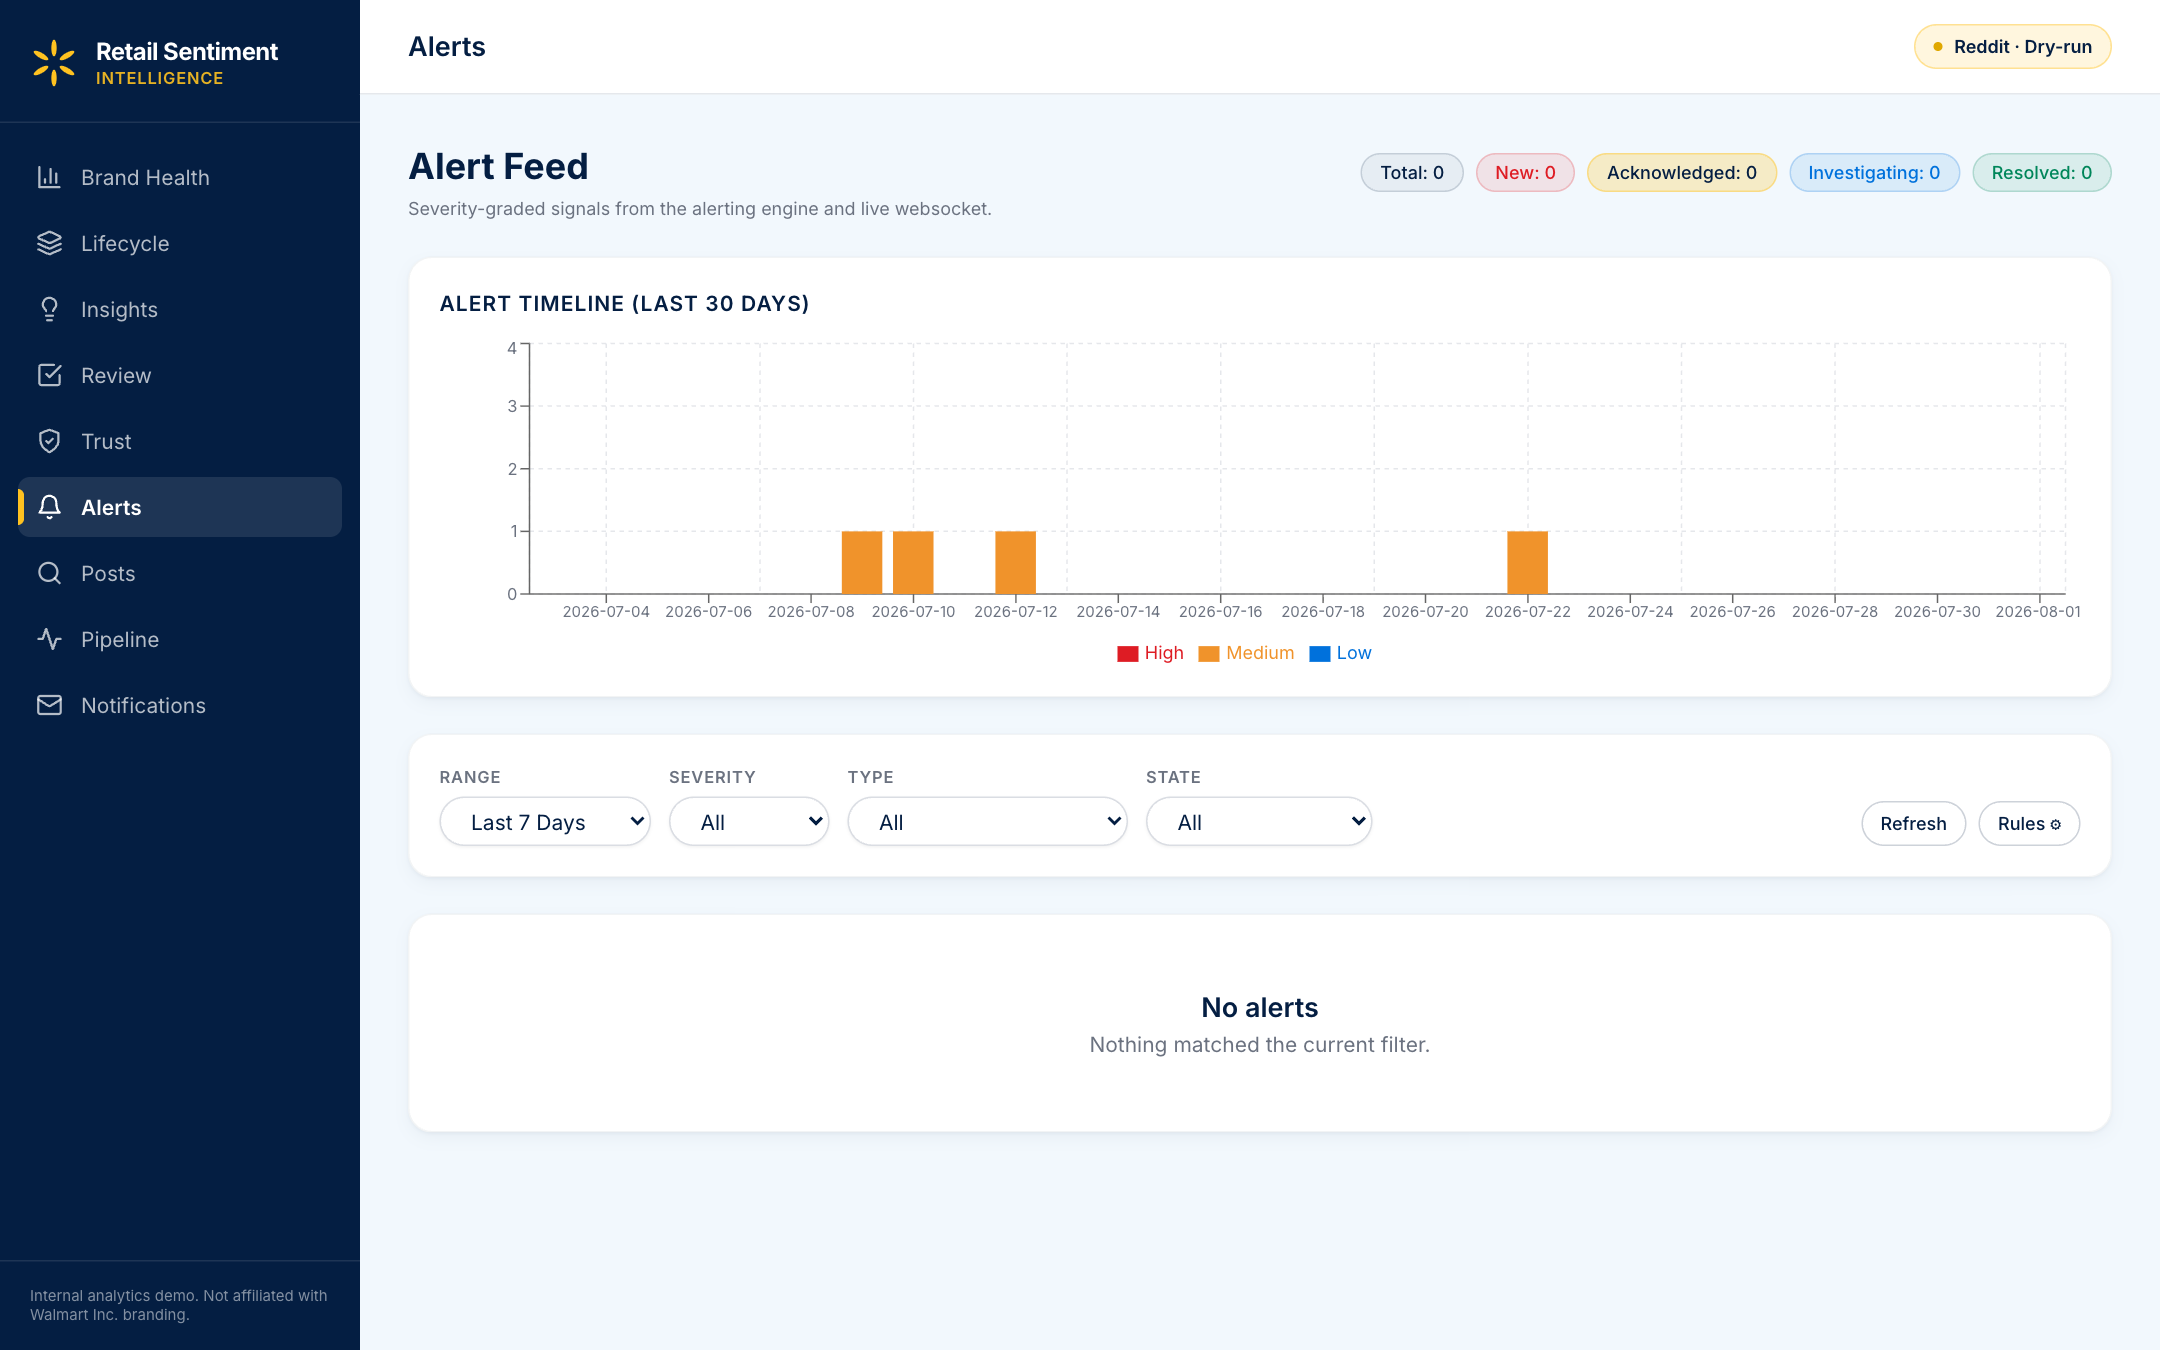
\includegraphics[width=\linewidth,height=0.82\textheight,keepaspectratio]{ui/alert_feed.png}
\caption{Alert Feed --- live P1/P2 stream sourced from the volume-spike
and sentiment-crash detectors of Listing~\ref{lst:alerts}.}\label{fig:ui:alerts}
\end{figure}

\section{Dashboard Overview}\label{sec:dash}
The dashboard is a Vite + React 18 + Tailwind SPA served by FastAPI.
Pages: Brand Health (KPIs and sentiment trend), Alert Feed (live P1/P2
stream), Post Explorer (multi-facet search), Review \& Validate (HITL
queue), Post Lifecycle (Kanban), Insights \& Competitor, Pipeline
Control, and Notifications.  The landing page is Brand Health
(Figure~\ref{fig:ui:brand}); the entire volume trend, sentiment gauge
and aspect breakdown are driven by the SQLite aggregates that
Listing~\ref{lst:alerts} also reads from, so what the analyst sees on
the dashboard is always the same view of the world that the alert engine
scored.

\begin{figure}[htbp]
\centering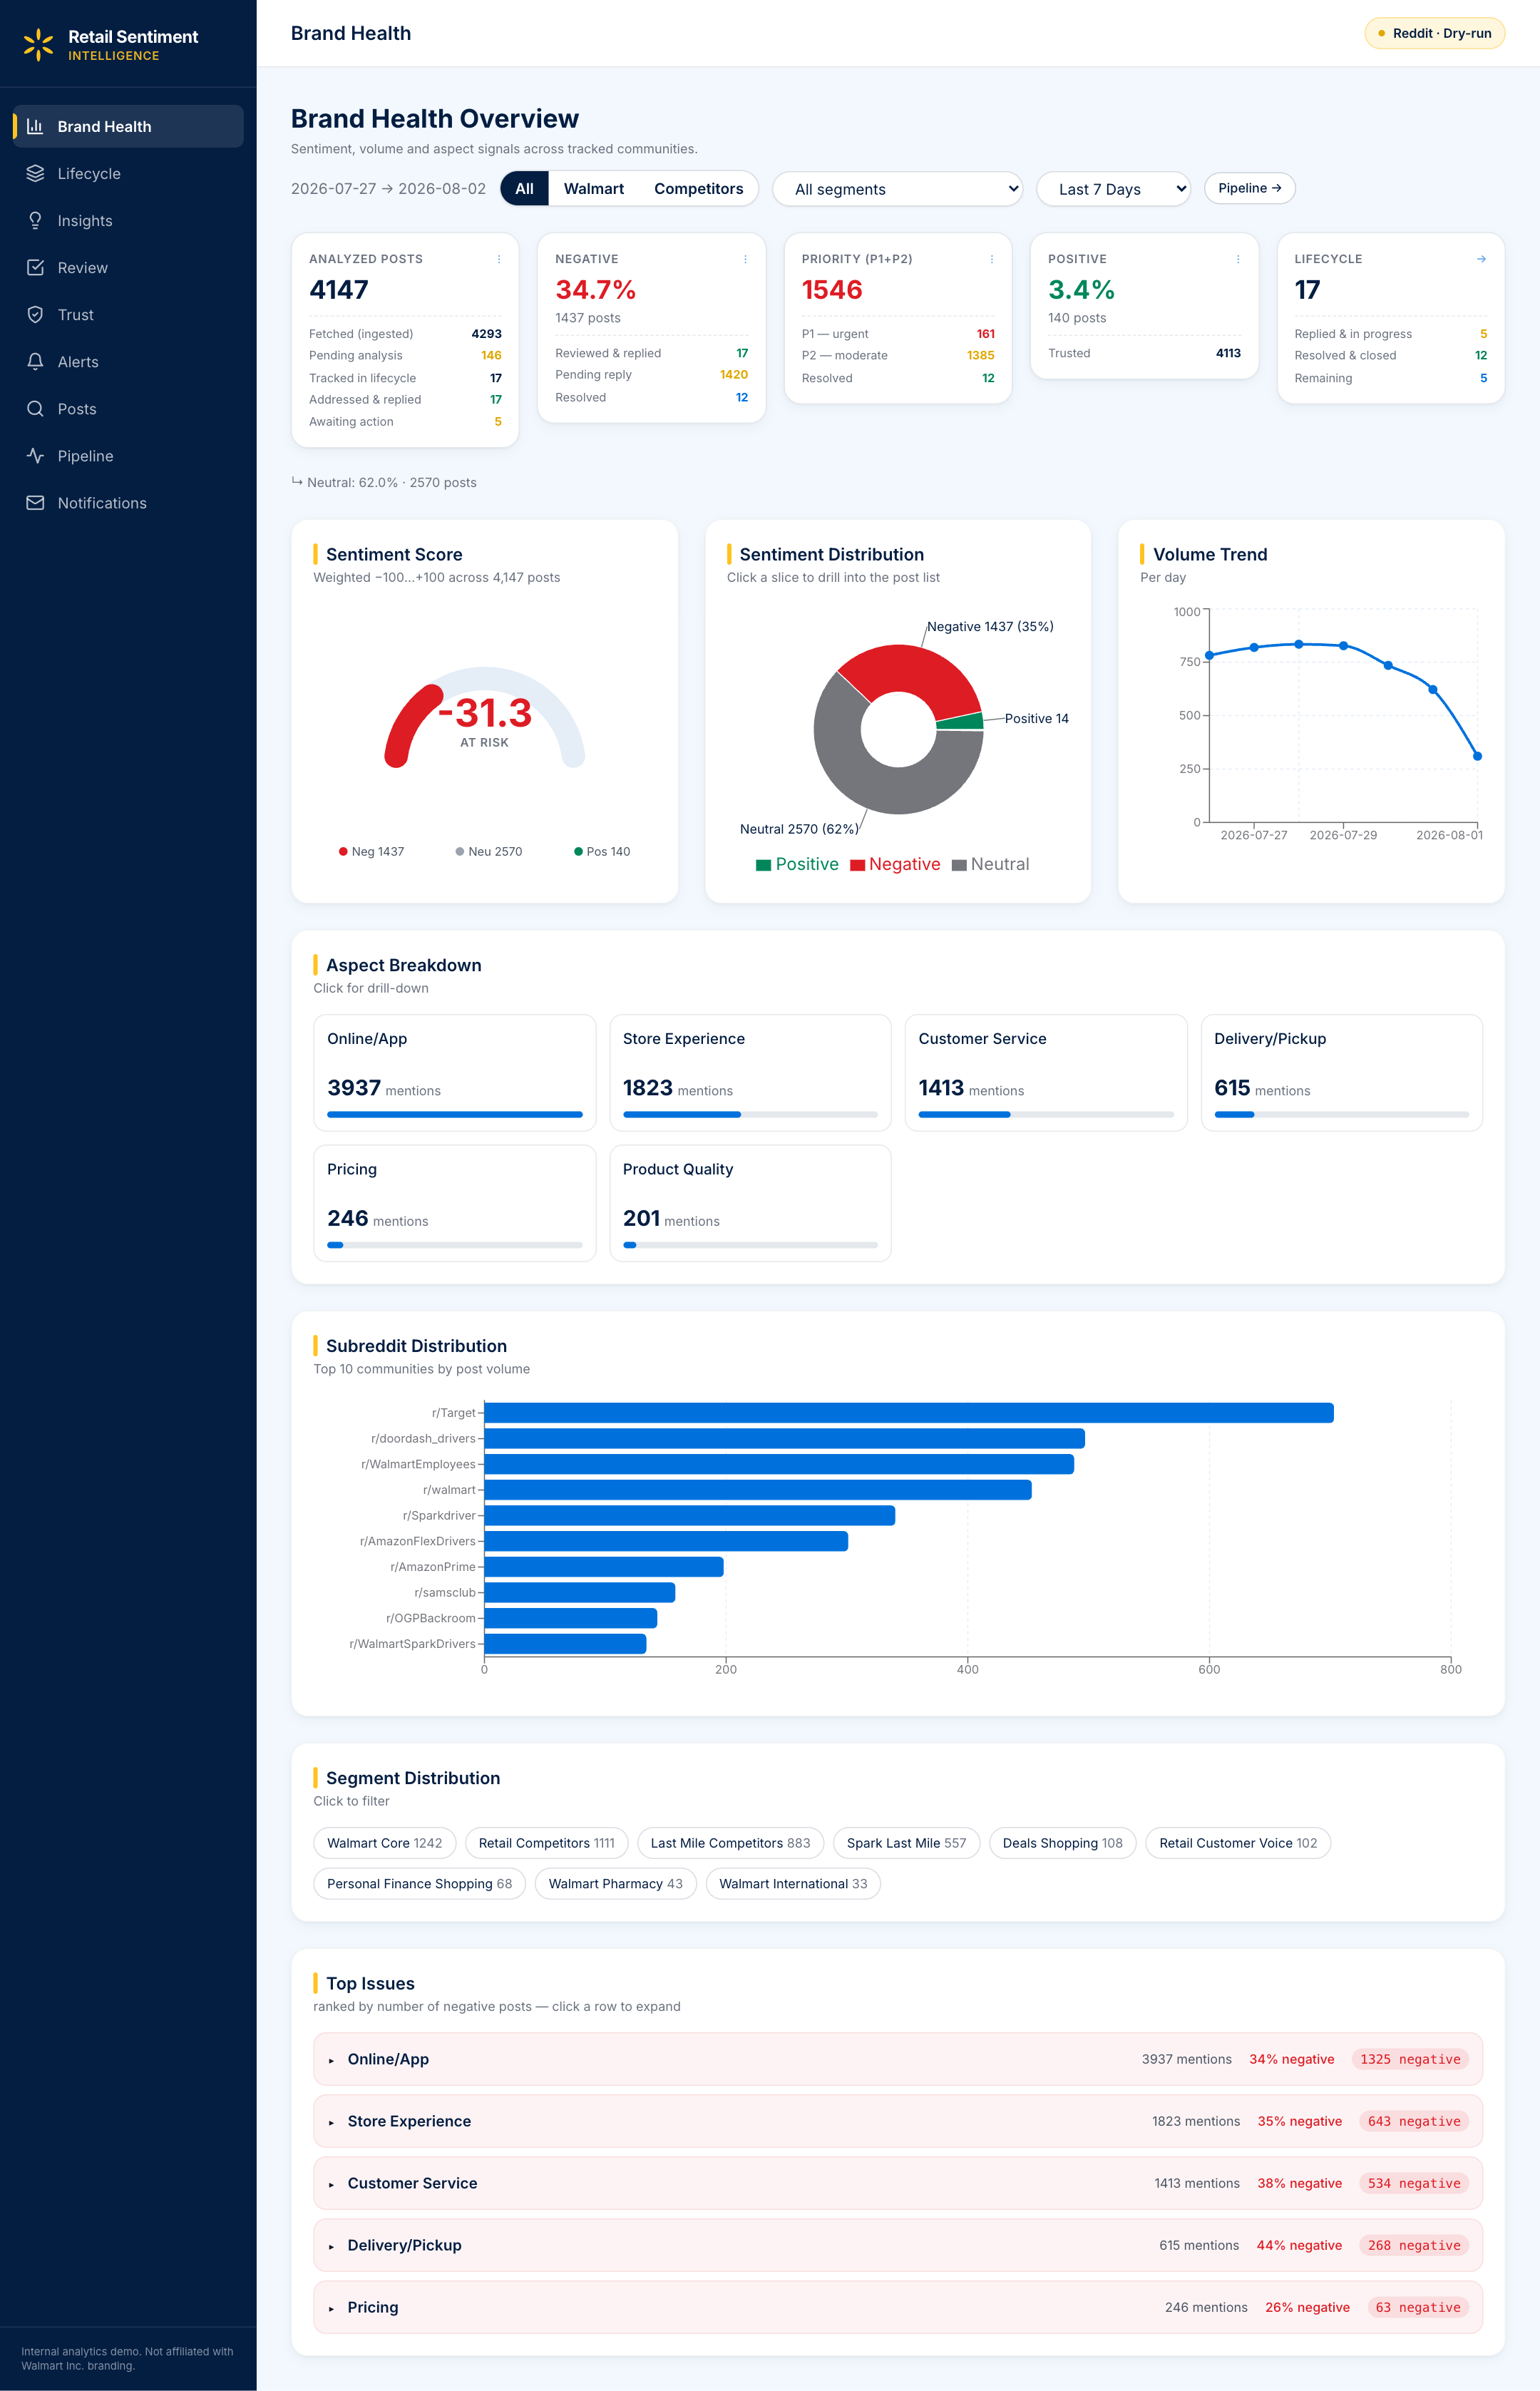
\includegraphics[width=\linewidth,height=0.82\textheight,keepaspectratio]{ui/brand_health.png}
\caption{Brand Health --- sentiment gauge, distribution donut, volume trend
and priority breakdown driven by the daily aggregates.}\label{fig:ui:brand}
\end{figure}

\section{Human-in-the-Loop Review \& Validate}\label{sec:hitl}
Every post landing in the review queue can be re-labelled (sentiment,
aspects), corrected (trust bucket), replied to (rule or LLM draft), and
closed with a resolution reason.  The workflow is shown in
Figure~\ref{fig:hitl}; the rendered queue is in
Figure~\ref{fig:ui:review}.  All actions are logged as
(post, before, after, analyst\_id, timestamp).  Listing~\ref{lst:review}
shows the endpoint that receives an analyst correction: it appends an
immutable feedback record \emph{and} rewrites the analysis so the
correction flows through to every downstream view --- Brand Health,
aspect drilldowns, Post Explorer and the Kanban board --- without any
extra re-aggregation call.

\begin{lstlisting}[caption={HITL correction endpoint: feedback audit log + live analysis rewrite ({\tt src/dashboard/api.py}).},label={lst:review}]
@app.post("/api/review/{post_id}")
def submit_review(post_id: str, correction: dict):
    _ensure_initialized()
    now = datetime.now(timezone.utc).isoformat()

    # 1. Immutable audit log (feedback table).
    feedback = {
        "id": f"fb_{post_id}_"
              f"{int(datetime.now(timezone.utc).timestamp())}",
        "post_id":             post_id,
        "analyst_id":          correction.get("analyst_id", "default"),
        "original_sentiment":  correction.get("original_sentiment"),
        "corrected_sentiment": correction.get("corrected_sentiment"),
        "original_aspects":    correction.get("original_aspects", []),
        "corrected_aspects":   correction.get("corrected_aspects", []),
        "trust_override":      correction.get("trust_override"),
        "notes":               correction.get("notes", ""),
        "created_at":          now,
        "partition_key":       correction.get("analyst_id", "default"),
    }
    _storage.upsert("feedback", feedback)

    # 2. Rewrite the analysis so the correction flows through to
    #    Brand Health, aspect drilldowns and the Kanban board.
    analysis = _storage.get_item("analyses",
                 f"analysis_{post_id}", correction.get("subreddit", ""))
    if analysis:
        if (c := correction.get("corrected_sentiment")):
            analysis["sentiment"]            = c
            analysis["sentiment_confidence"] = 1.0     # human-validated
        if isinstance(correction.get("corrected_aspects"), list):
            analysis["aspects"] = [
                {"aspect": a, "confidence": 1.0} if isinstance(a, str)
                else a for a in correction["corrected_aspects"]]
        if (t := correction.get("trust_override")) is not None:
            analysis["trust_score"]    = max(0.0, min(1.0, float(t)))
            analysis["trust_override"] = True
        analysis["needs_review"]    = False
        analysis["human_validated"] = True
        analysis["validated_at"]    = now
        analysis["validated_by"]    = correction.get("analyst_id", "default")
        _storage.upsert("analyses", analysis)

    return {"status": "saved", "feedback_id": feedback["id"],
            "analysis_updated": analysis is not None}
\end{lstlisting}

\begin{figure}[htbp]
\centering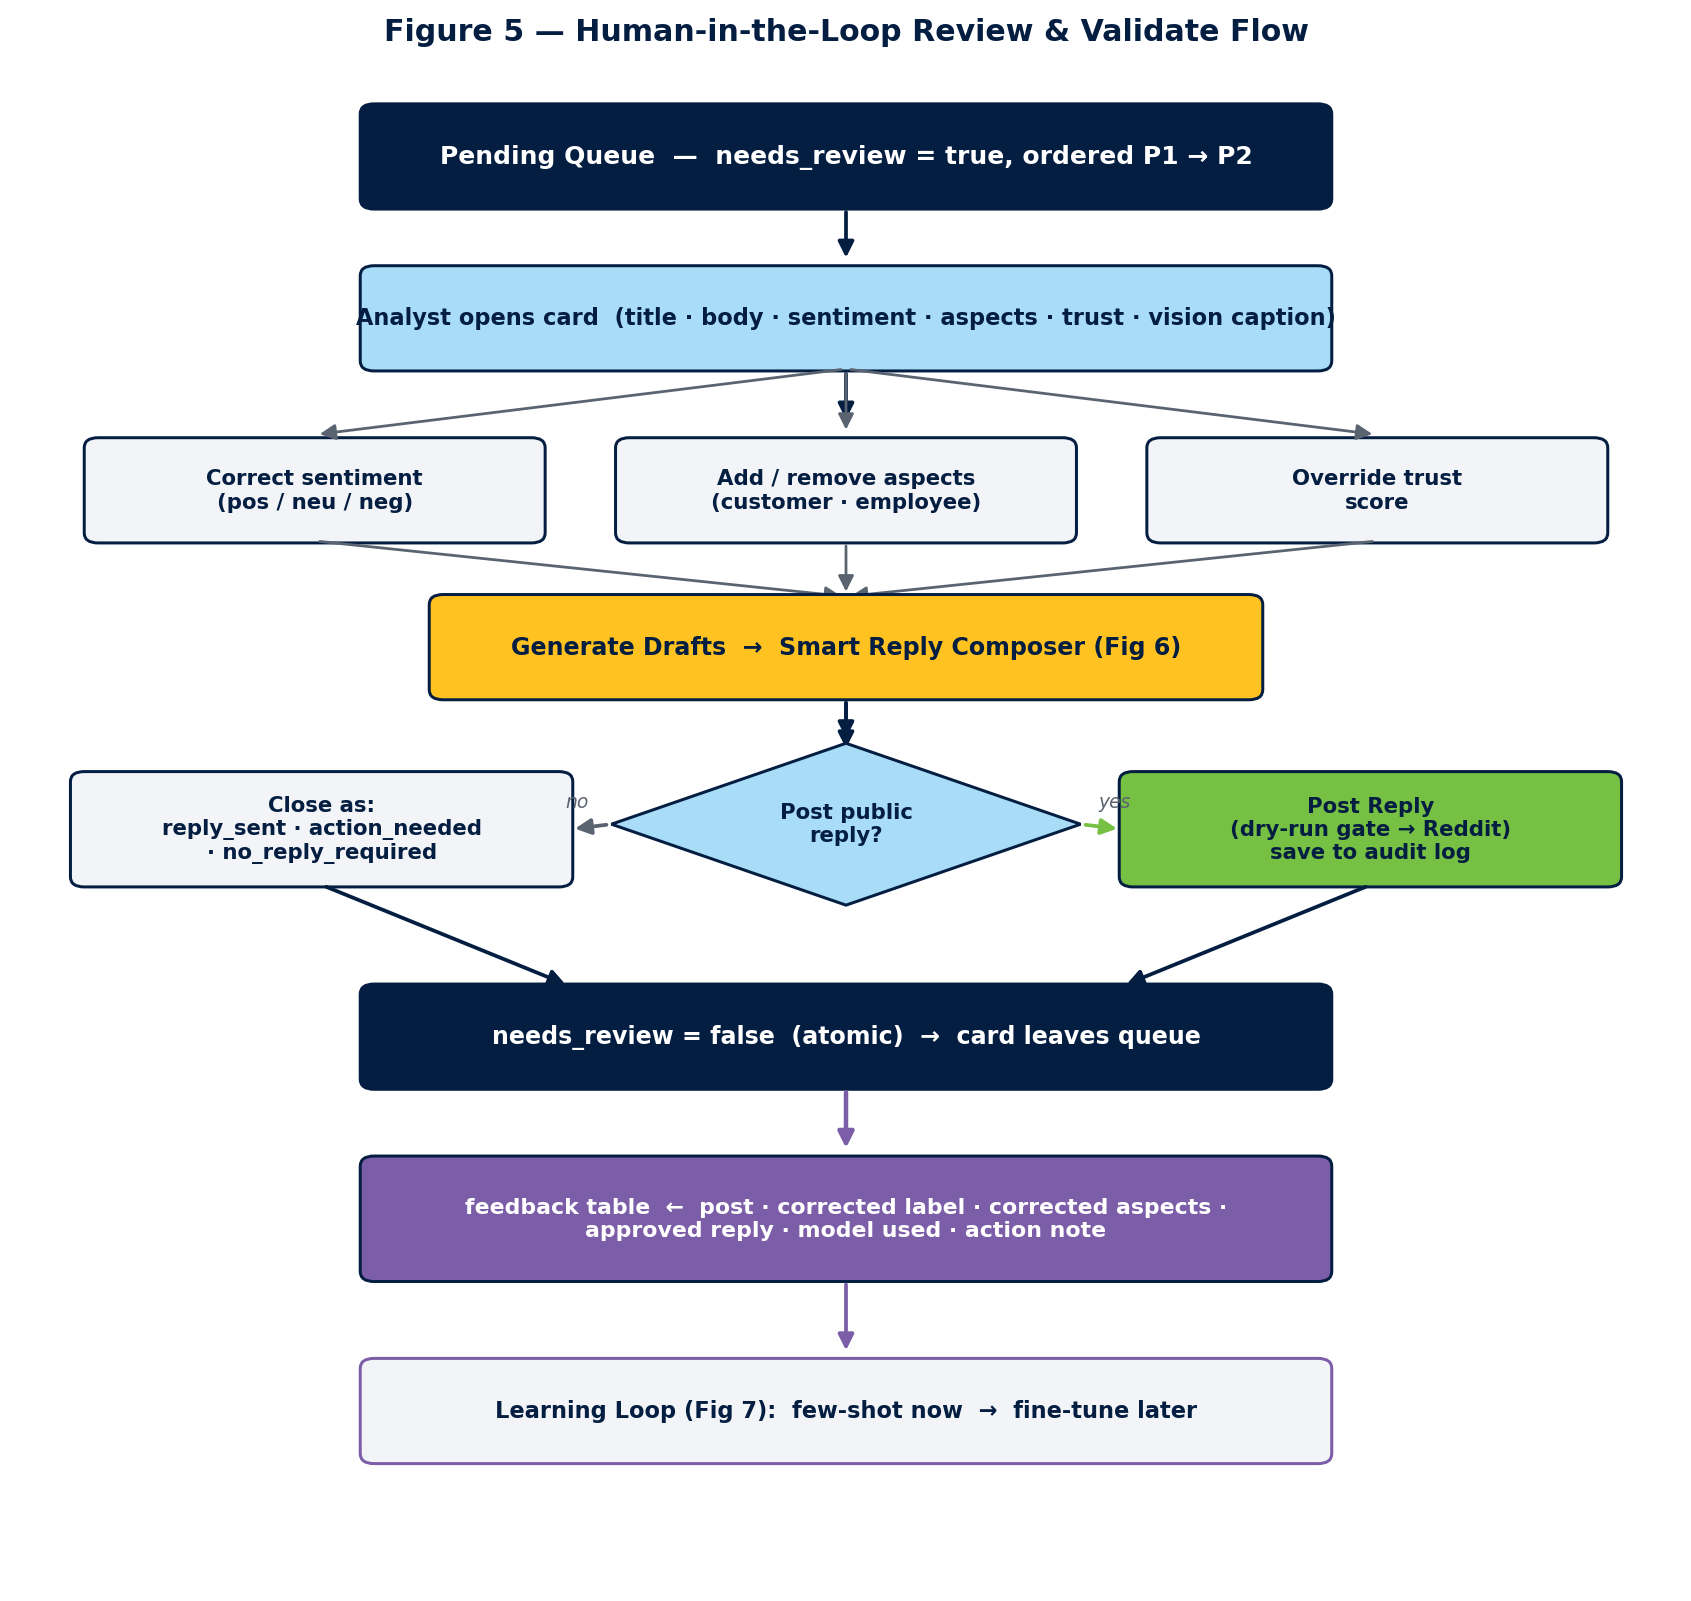
\includegraphics[width=\linewidth]{fig5_review_validate_flow}
\caption{Human-in-the-loop Review \& Validate flow.}\label{fig:hitl}
\end{figure}

\begin{figure}[htbp]
\centering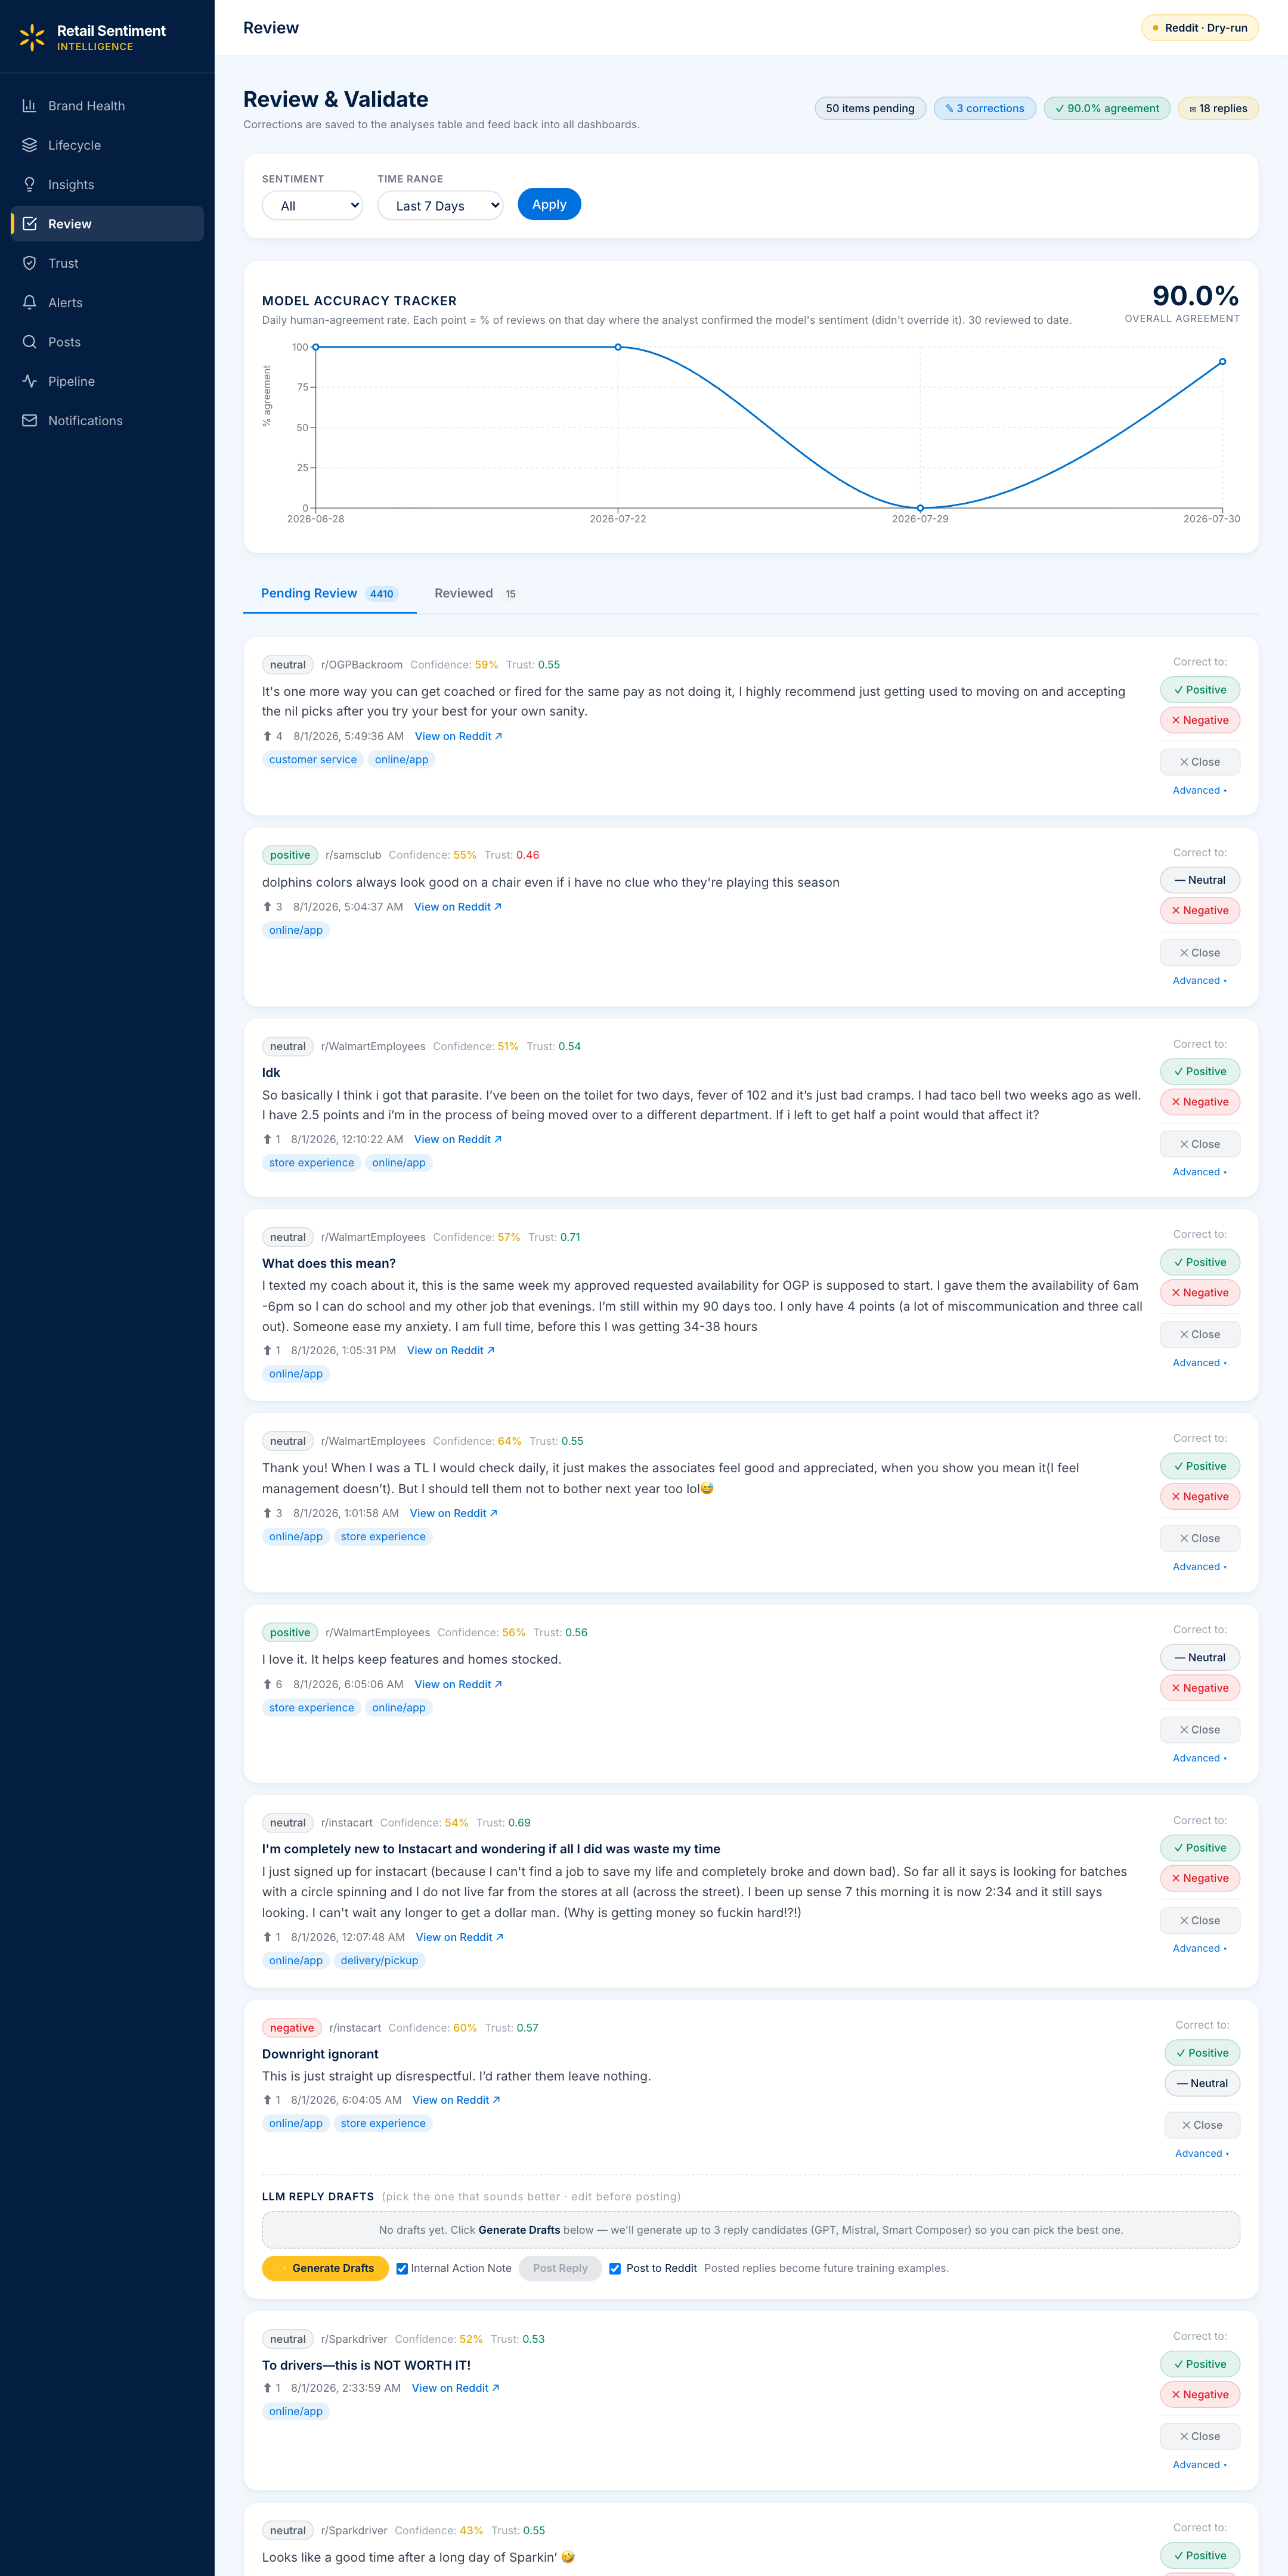
\includegraphics[width=\linewidth,height=0.82\textheight,keepaspectratio]{ui/review_validate.png}
\caption{Review \& Validate queue --- posts flagged by the model land here;
analysts re-label sentiment/aspects and either compose a reply or resolve
in place.  Corrections are POSTed to the endpoint in
Listing~\ref{lst:review}.}\label{fig:ui:review}
\end{figure}

\section{Smart Reply Composer --- Dual-Draft (Rule + LLM)}\label{sec:reply}
The reply composer offers two drafts side-by-side: a rule-based template
that guarantees policy compliance, and an LLM-generated draft that
personalises to the post's aspects and sentiment.  Few-shot examples come
from the last analyst-posted replies pulled straight from the feedback
store --- this is what closes the learning loop of \S\ref{sec:loop}
without any offline retraining.  Listing~\ref{lst:reply} shows the endpoint
that ties it together.  See Figure~\ref{fig:reply}.

\begin{lstlisting}[caption={Dual-draft reply endpoint (rule + LLM, few-shot from posted replies) ({\tt src/dashboard/api.py}).},label={lst:reply}]
@app.post("/api/review/{post_id}/draft-reply")
def draft_reply(post_id: str, payload: dict | None = None):
    """Generate a customer-specific reply draft. Uses the last N
    analyst-posted replies as few-shot examples --- every posted
    reply becomes training context for future drafts."""
    _ensure_initialized()
    payload = payload or {}
    subredd = payload.get("subreddit", "")

    analysis = _storage.get_item("analyses",
                                 f"analysis_{post_id}", subredd)
    if not analysis:
        return {"status": "error", "reason": "analysis_not_found"}
    if analysis.get("sentiment") != "negative":
        return {"status": "error", "reason": "not_negative"}

    raw      = _storage.get_item("raw_posts", post_id, subredd) or {}
    aspects  = _aspect_names(analysis.get("aspects", []))
    examples = _collect_reply_examples(limit=5)      # <-- few-shot

    llm    = _get_reply_llm()
    result = llm.generate_reply_pair(
        post_title=raw.get("title", ""),
        post_text =raw.get("body",  "") or raw.get("title", ""),
        subreddit =analysis.get("subreddit", ""),
        author    =raw.get("author", ""),
        aspects   =aspects,
        examples  =examples)

    drafts  = result.get("drafts", [])       # rule + LLM
    primary = drafts[0] if drafts else {}
    return {"status": "ok", "drafts": drafts,
            "reply":         primary.get("reply", ""),
            "model_used":    primary.get("model_used", ""),
            "source":        primary.get("source", ""),
            "examples_used": len(examples)}
\end{lstlisting}

\begin{figure}[htbp]
\centering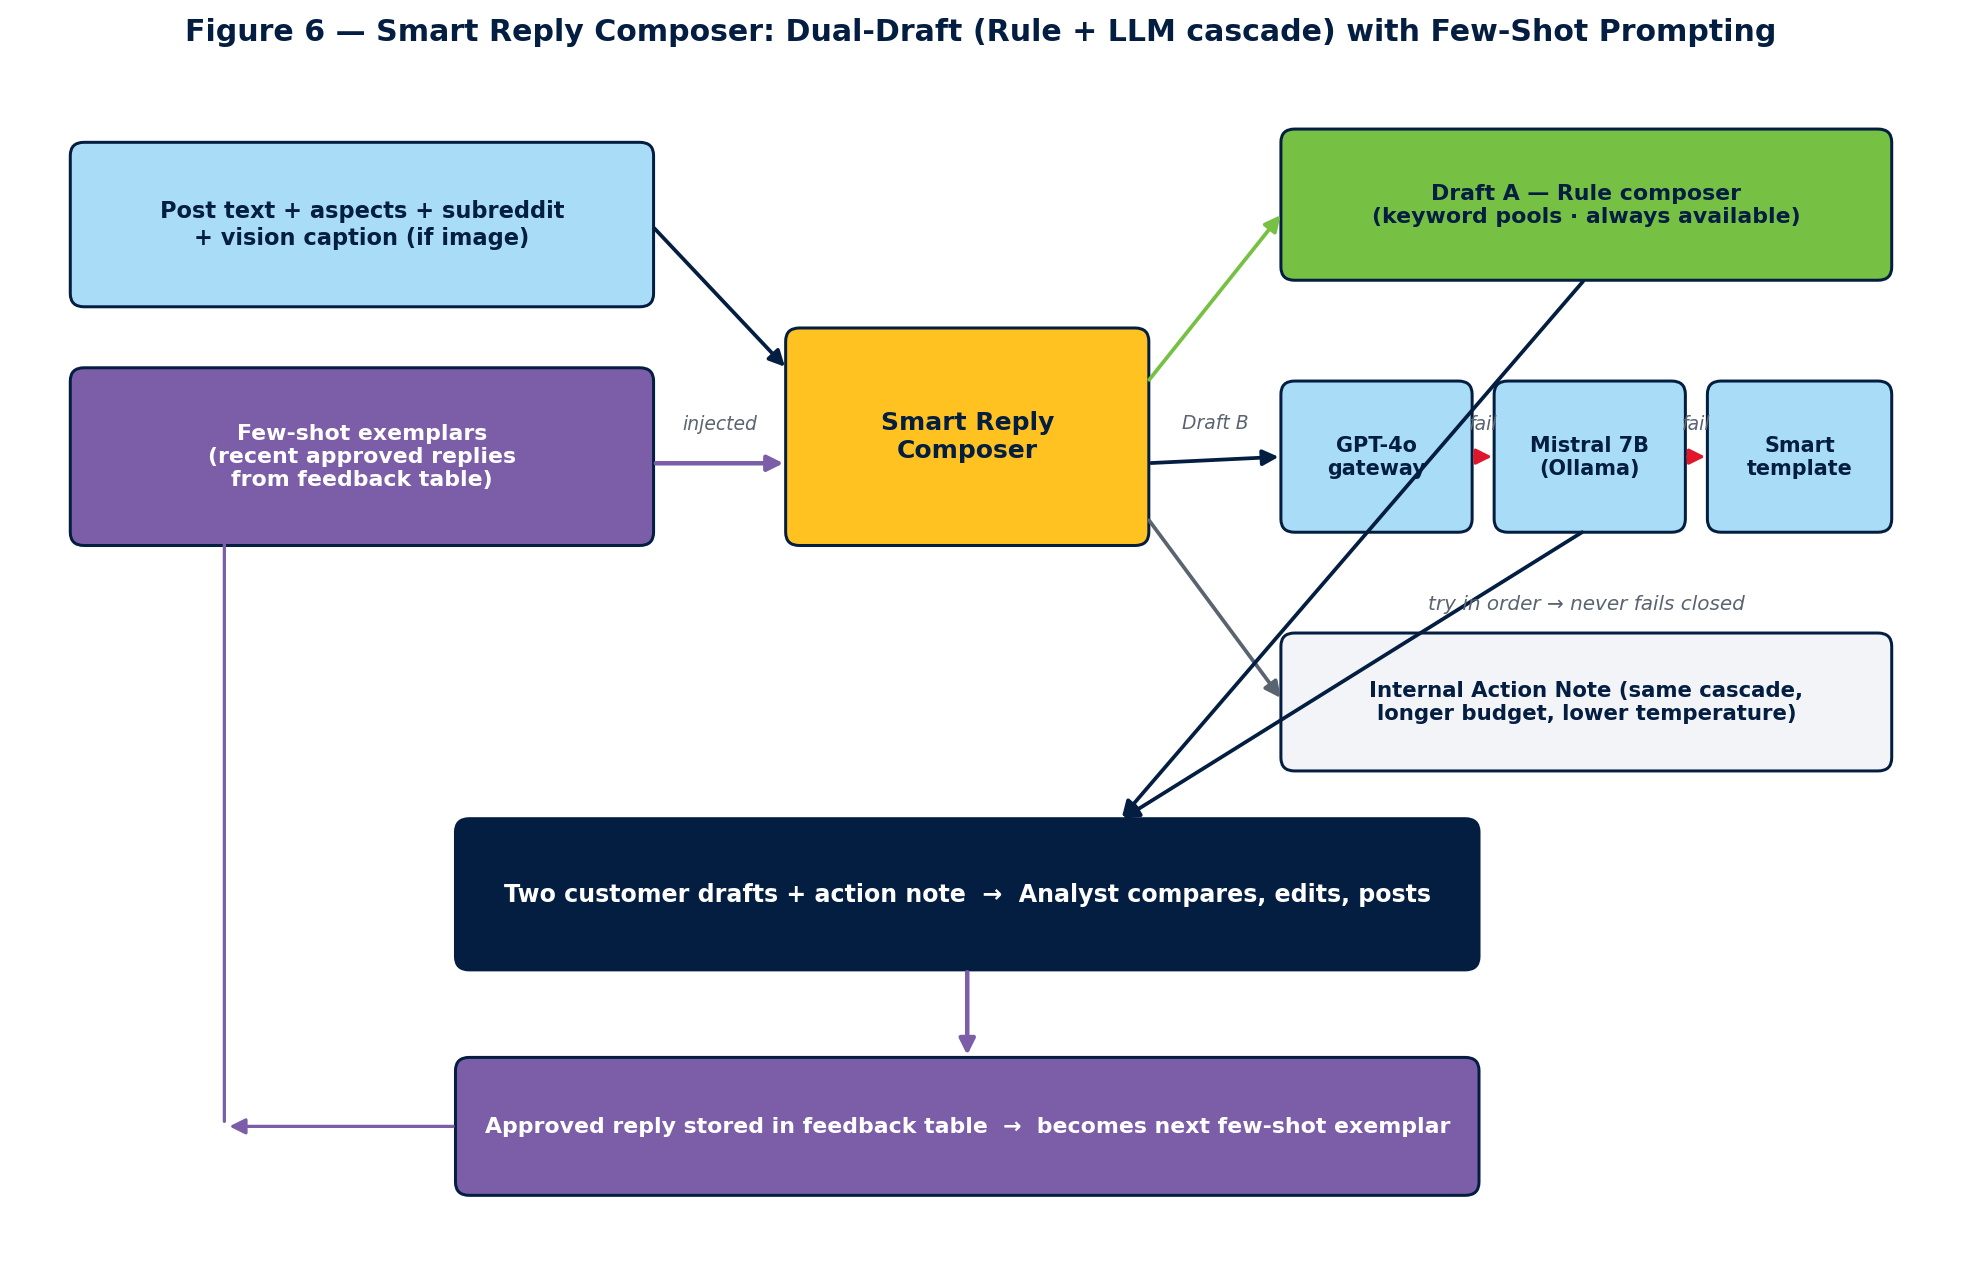
\includegraphics[width=\linewidth]{fig6_reply_cascade}
\caption{Smart Reply Composer --- dual-draft with few-shot.}\label{fig:reply}
\end{figure}

\section{Learning Loop --- Feedback for Future Retraining}\label{sec:loop}
Corrections and posted replies stream into the feedback store keyed by
post\_id and model version (the same audit log written by
Listing~\ref{lst:review}).  A weekly export produces training pairs for
sentiment (correction $\to$ label) and reply generation (post $\to$
posted-reply).  Figure~\ref{fig:loop} depicts the loop and the path to
future auto-reply --- the same few-shot pull in Listing~\ref{lst:reply}
means the composer becomes measurably better every week without touching
the model weights.

\begin{figure}[htbp]
\centering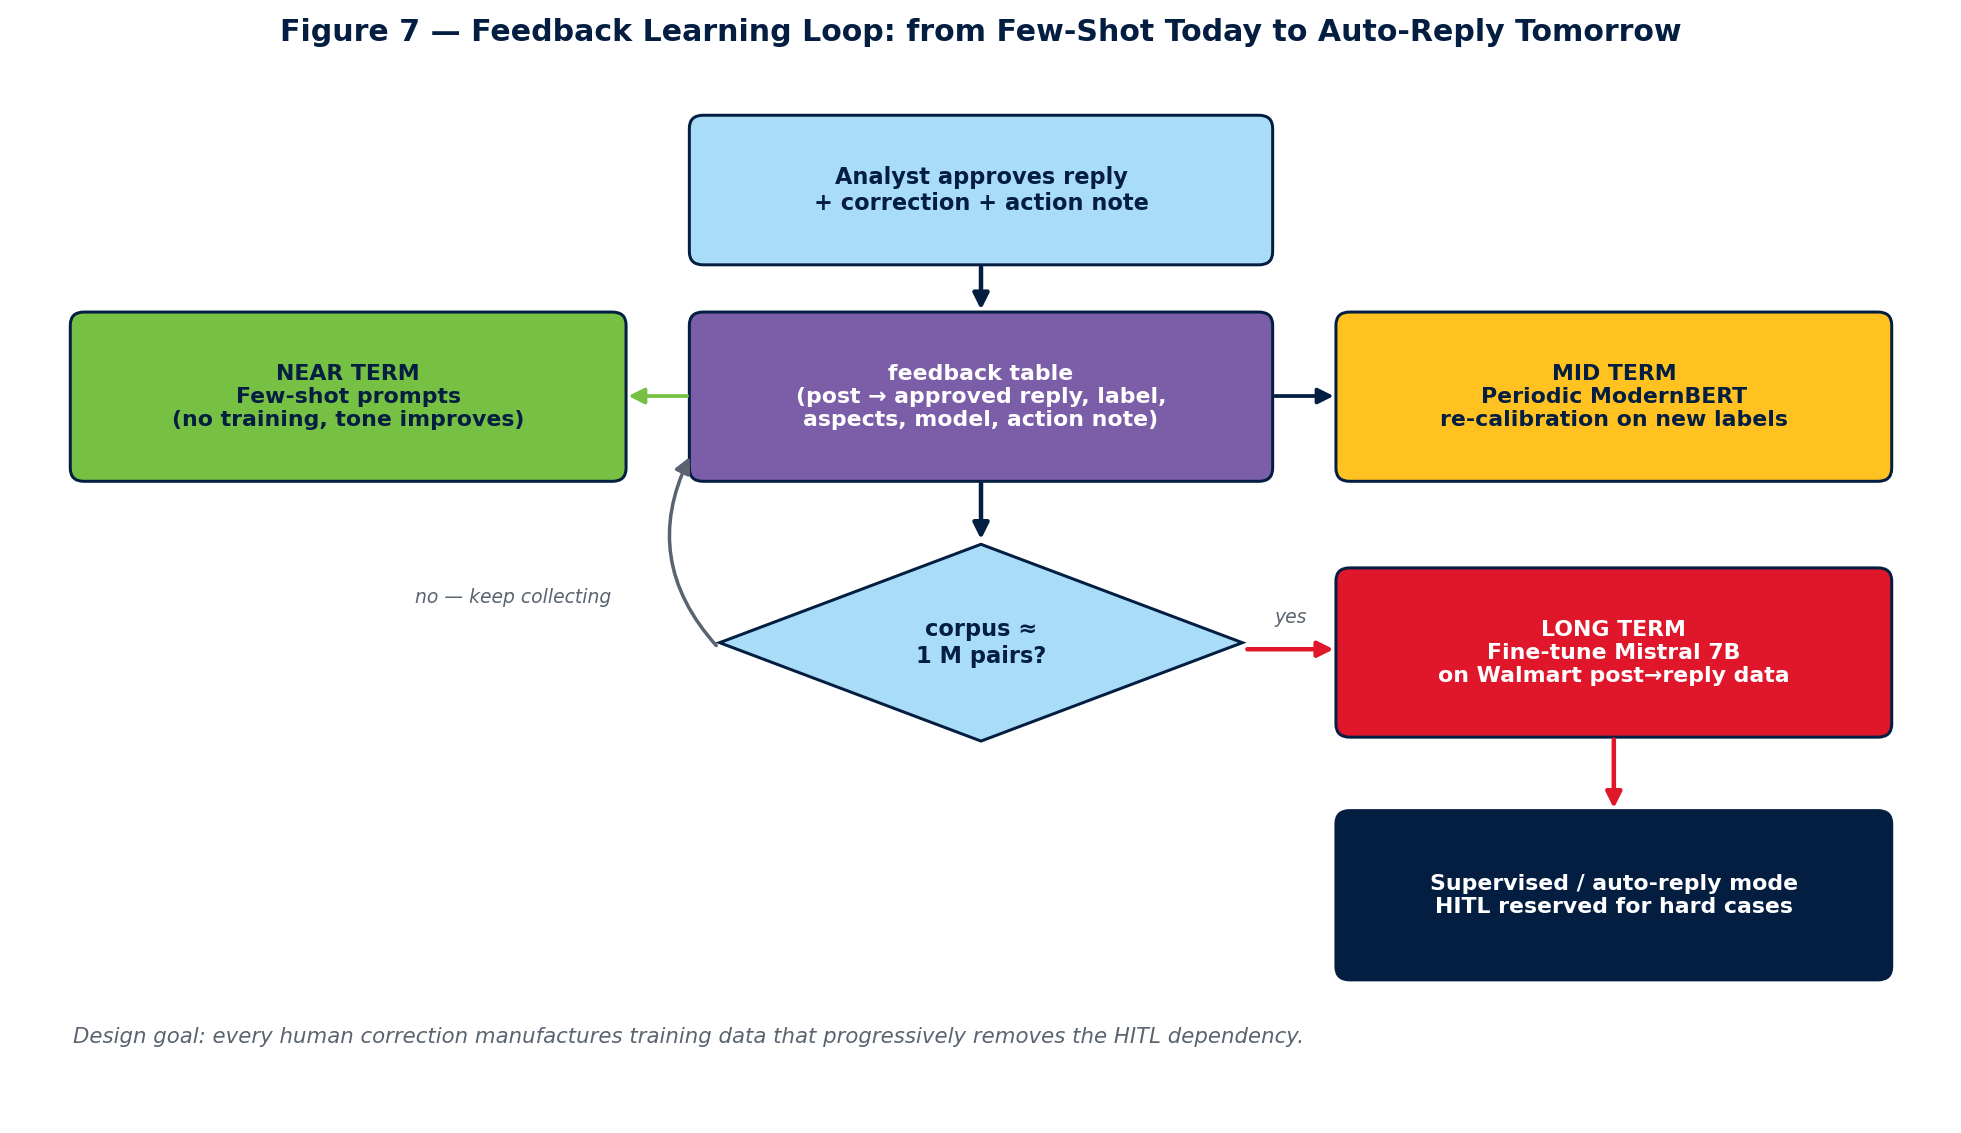
\includegraphics[width=\linewidth]{fig7_learning_loop}
\caption{Feedback learning loop and path to auto-reply.}\label{fig:loop}
\end{figure}

\section{Post Explorer and Multi-Facet Search}\label{sec:explore}
Post Explorer supports filters over subreddit, aspect, sentiment, trust
bucket, priority tier, resolution state, date range, and free-text.
Figure~\ref{fig:ui:posts} shows the rendered page; every filter is a
query parameter on the same \texttt{/api/posts} endpoint that the Kanban
and Review queues also read, so an analyst can navigate freely between
the three views without ever seeing an inconsistent post state.

\begin{figure}[htbp]
\centering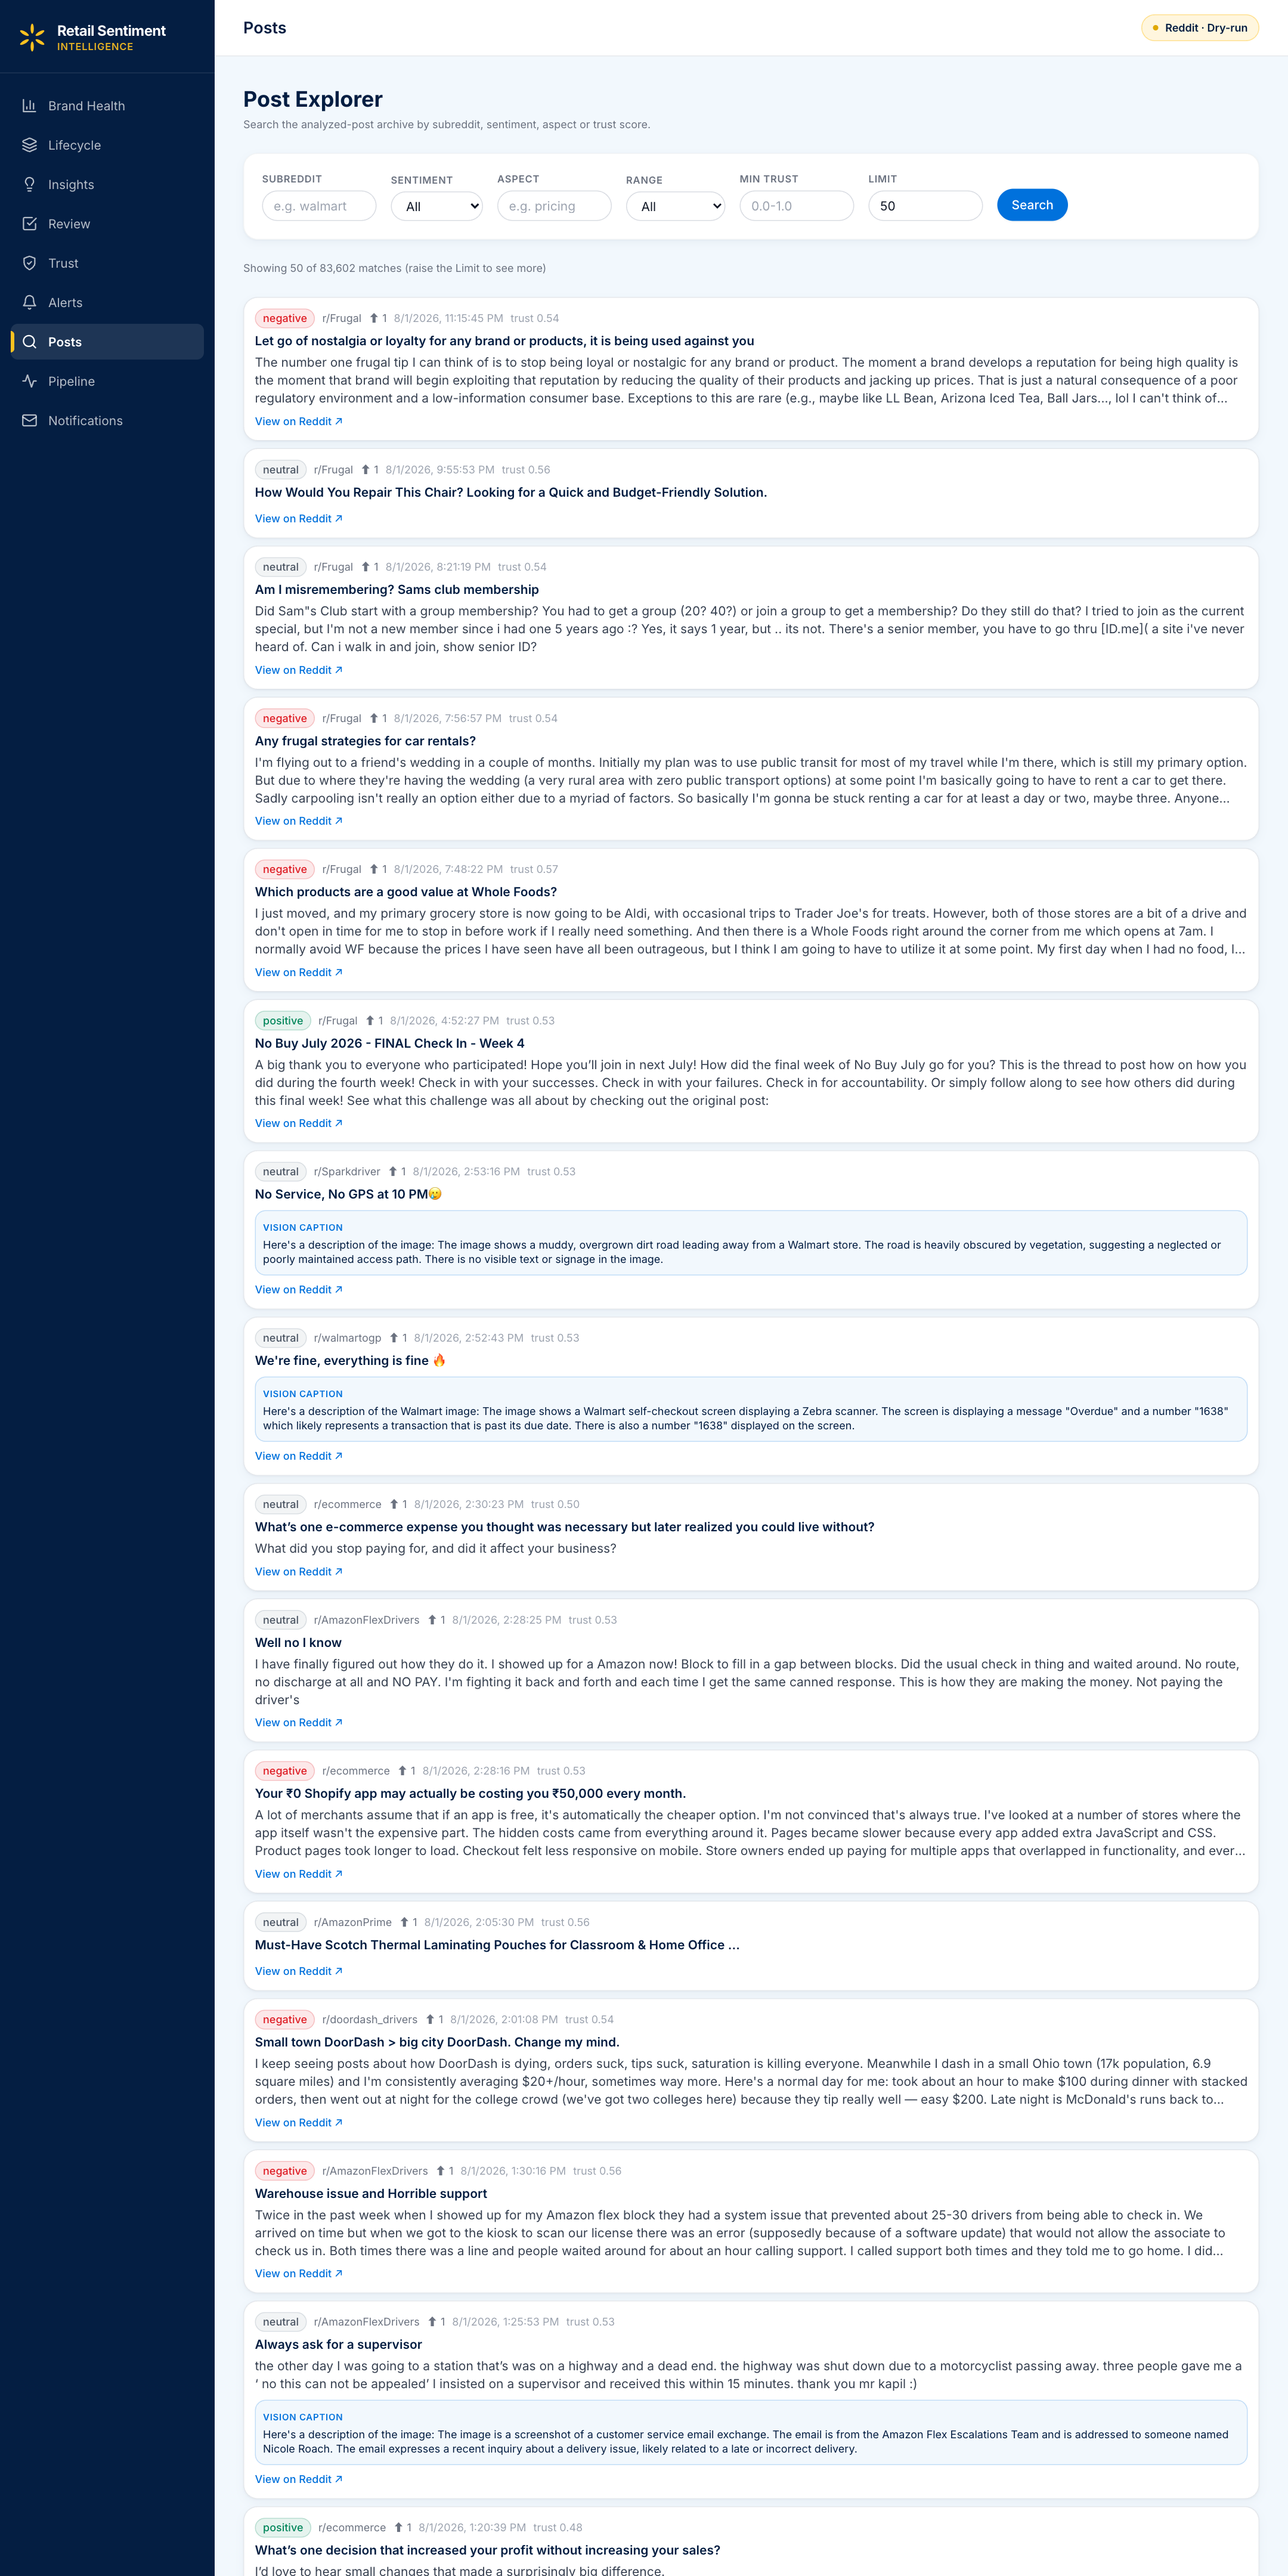
\includegraphics[width=\linewidth,height=0.82\textheight,keepaspectratio]{ui/post_explorer.png}
\caption{Post Explorer --- multi-facet search over subreddit, aspect,
sentiment, trust bucket, priority tier and free text.}\label{fig:ui:posts}
\end{figure}

\section{Post Lifecycle (Kanban Workflow)}\label{sec:kanban}
Every P1/P2 alert flows through a Kanban board with four states
(Triaged $\to$ Acknowledged $\to$ In Progress $\to$ Resolved).  See
Figure~\ref{fig:kanban} for the state machine and
Figure~\ref{fig:ui:kanban} for the rendered board.  State transitions
carry SLA timestamps so we can compute time-to-acknowledge and
time-to-resolve.

\begin{figure}[htbp]
\centering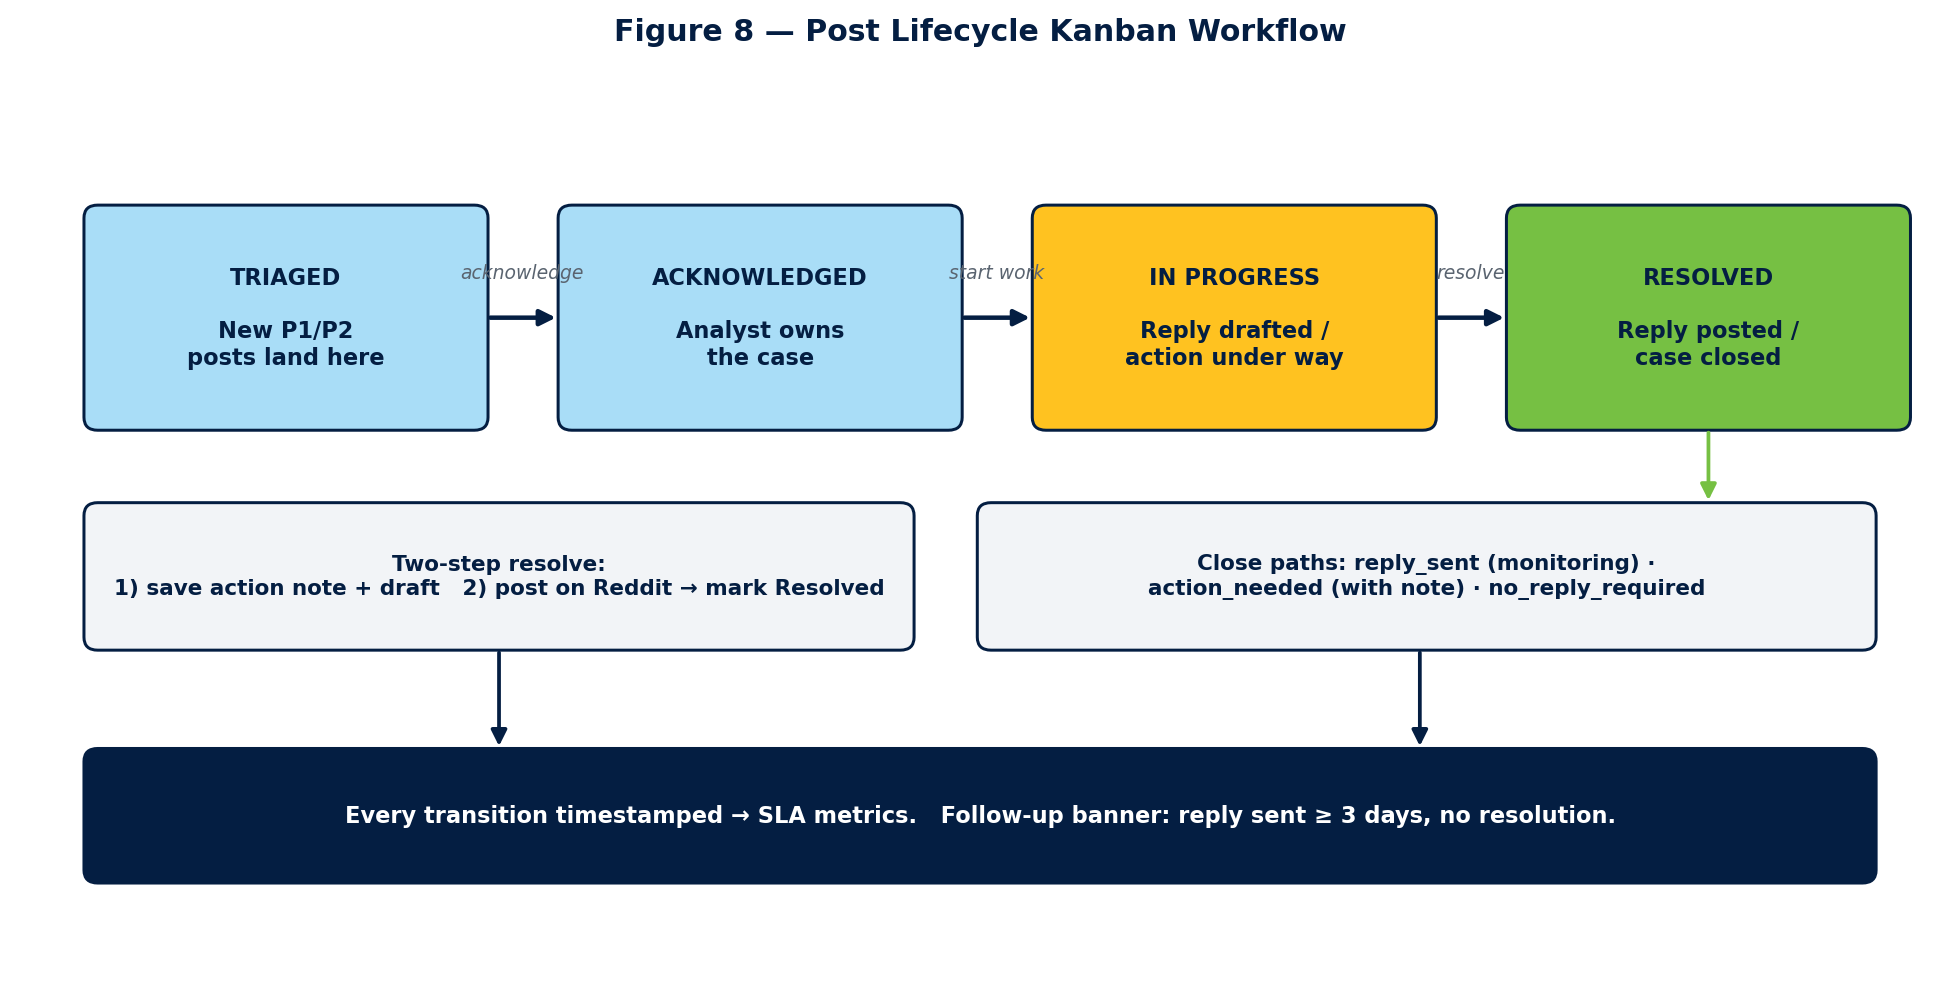
\includegraphics[width=\linewidth]{fig8_lifecycle_kanban}
\caption{Post Lifecycle Kanban workflow.}\label{fig:kanban}
\end{figure}

\begin{figure}[htbp]
\centering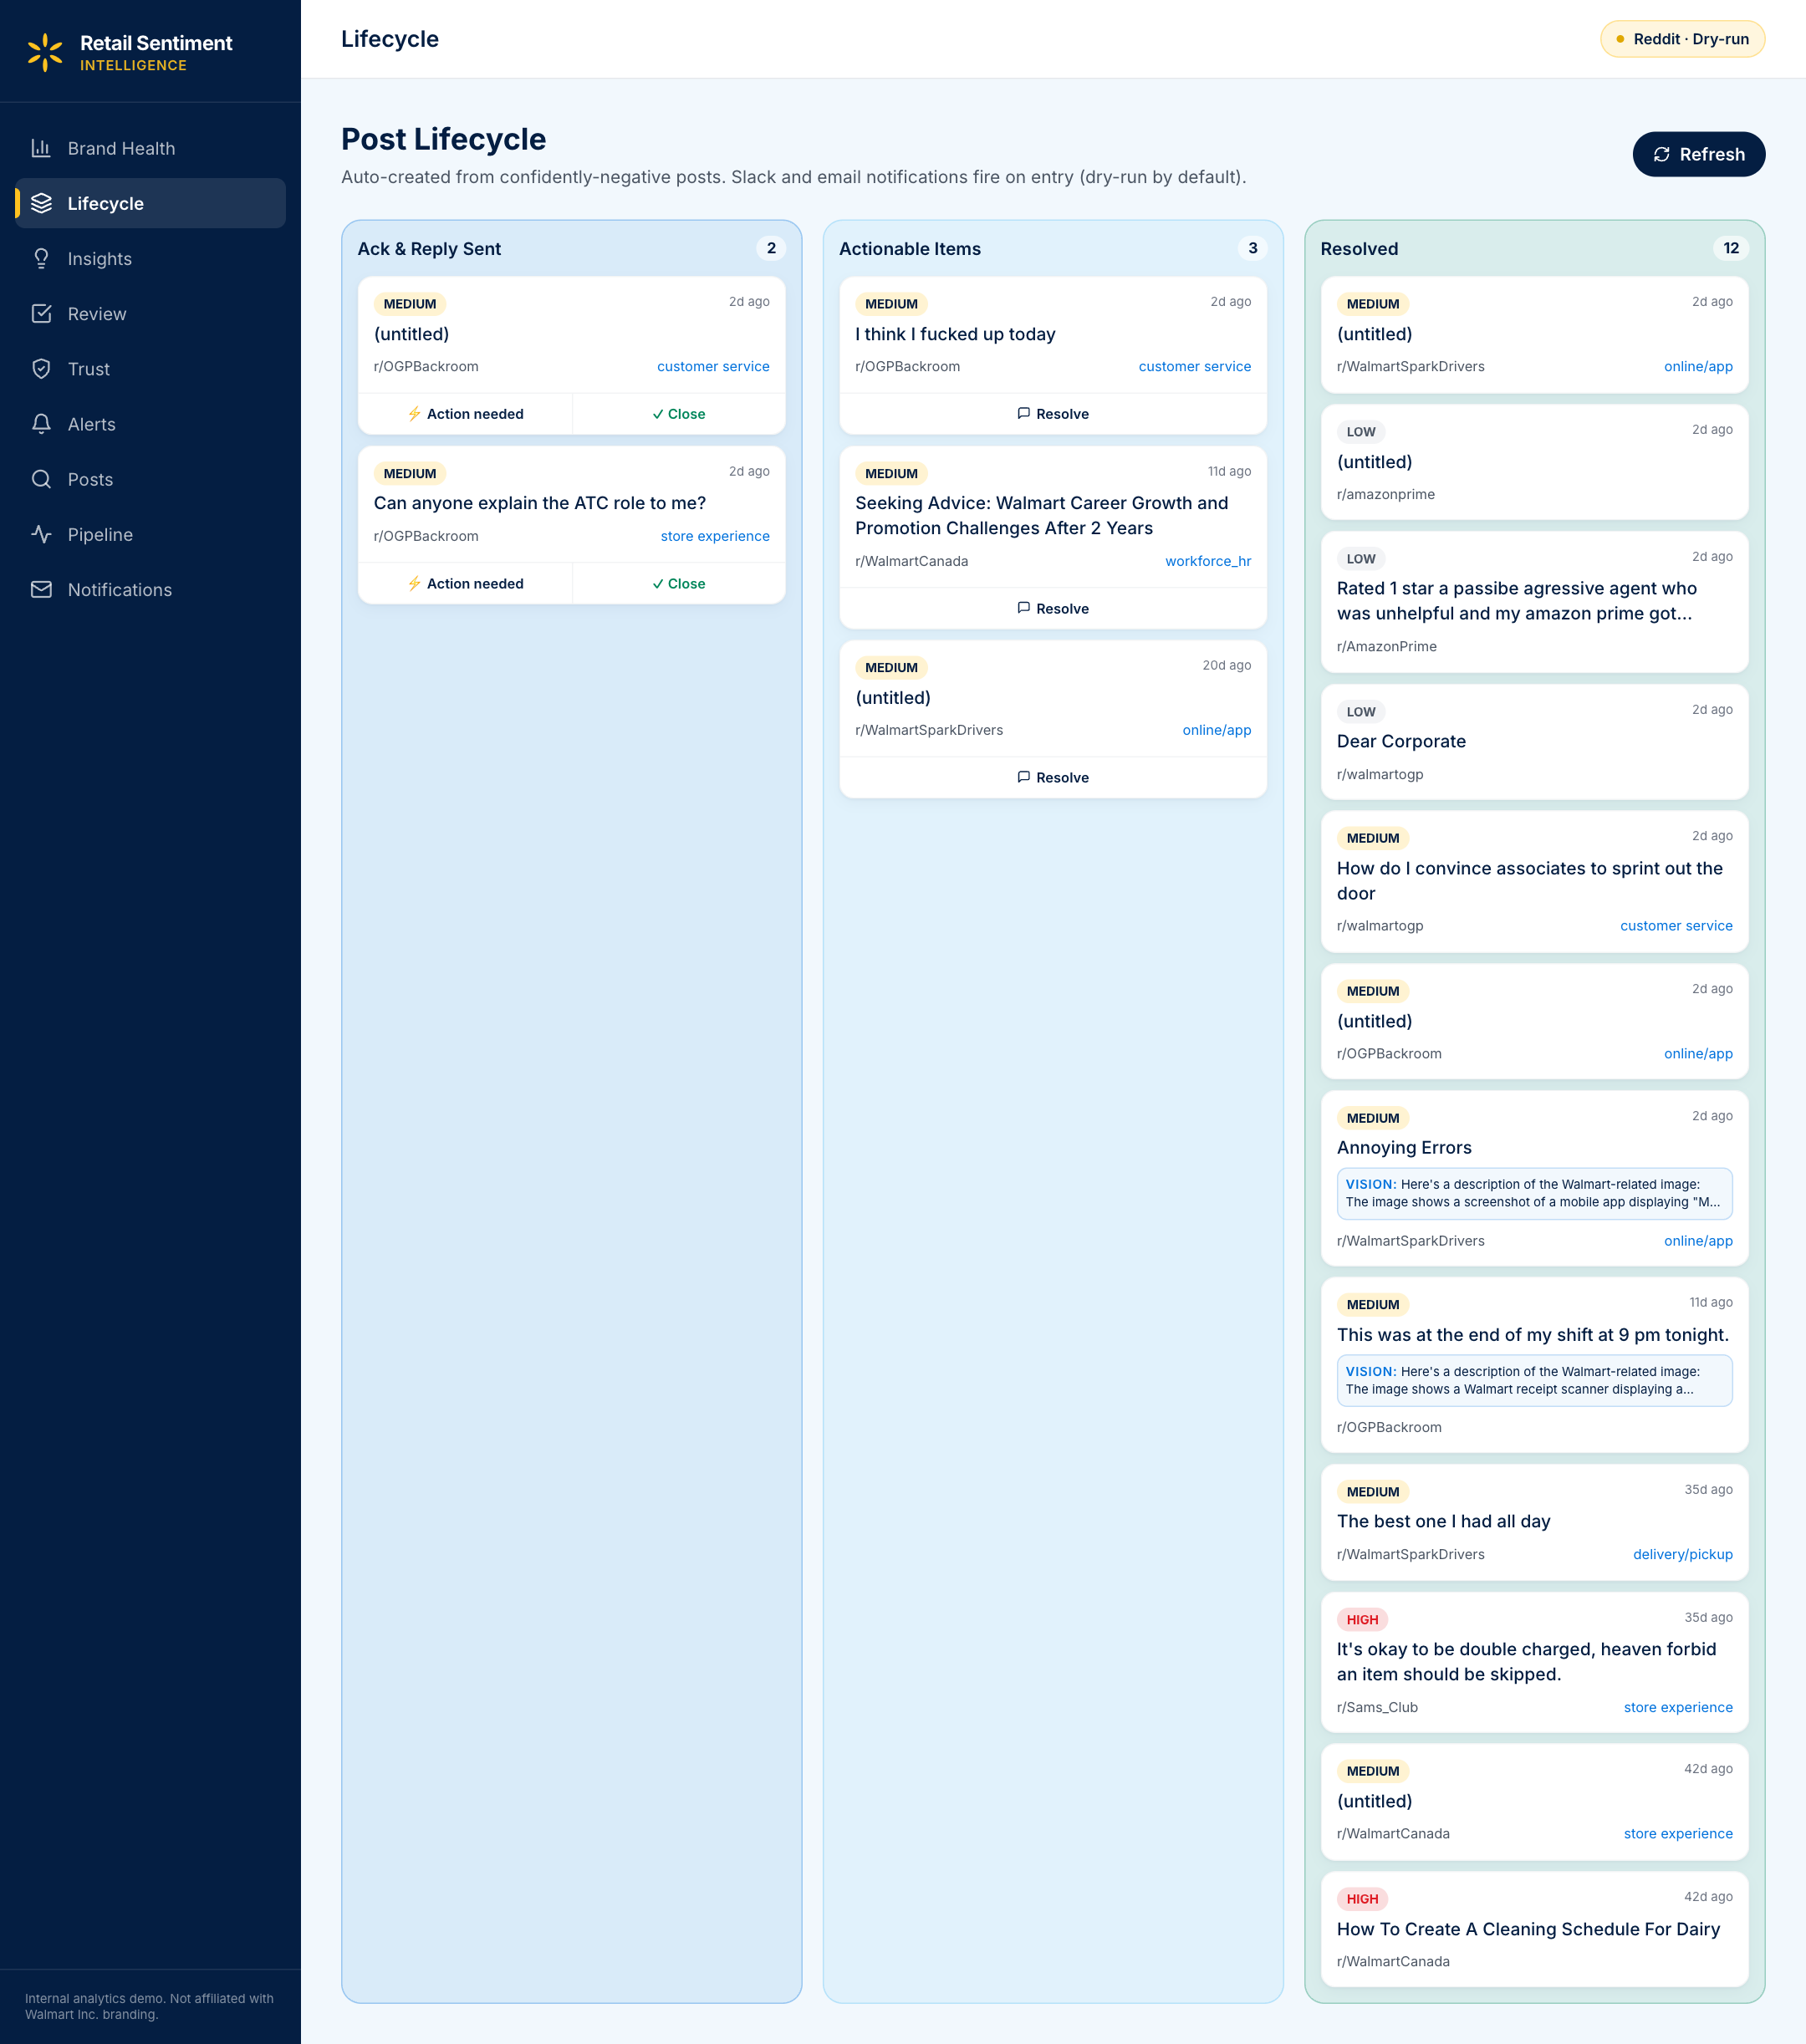
\includegraphics[width=\linewidth,height=0.82\textheight,keepaspectratio]{ui/lifecycle_kanban.png}
\caption{Post Lifecycle --- Kanban board with SLA timestamps for every
transition.}\label{fig:ui:kanban}
\end{figure}

\section{Insights and Competitor Analysis}\label{sec:insights}
The Insights page shows aspect-level negative-share for Walmart vs.\ a
curated set of competitor communities (Target, Costco, Amazon, Kroger,
Aldi) so analysts can distinguish a company-specific issue from an
industry trend.  Figure~\ref{fig:ui:insights} shows the rendered view.

\begin{figure}[htbp]
\centering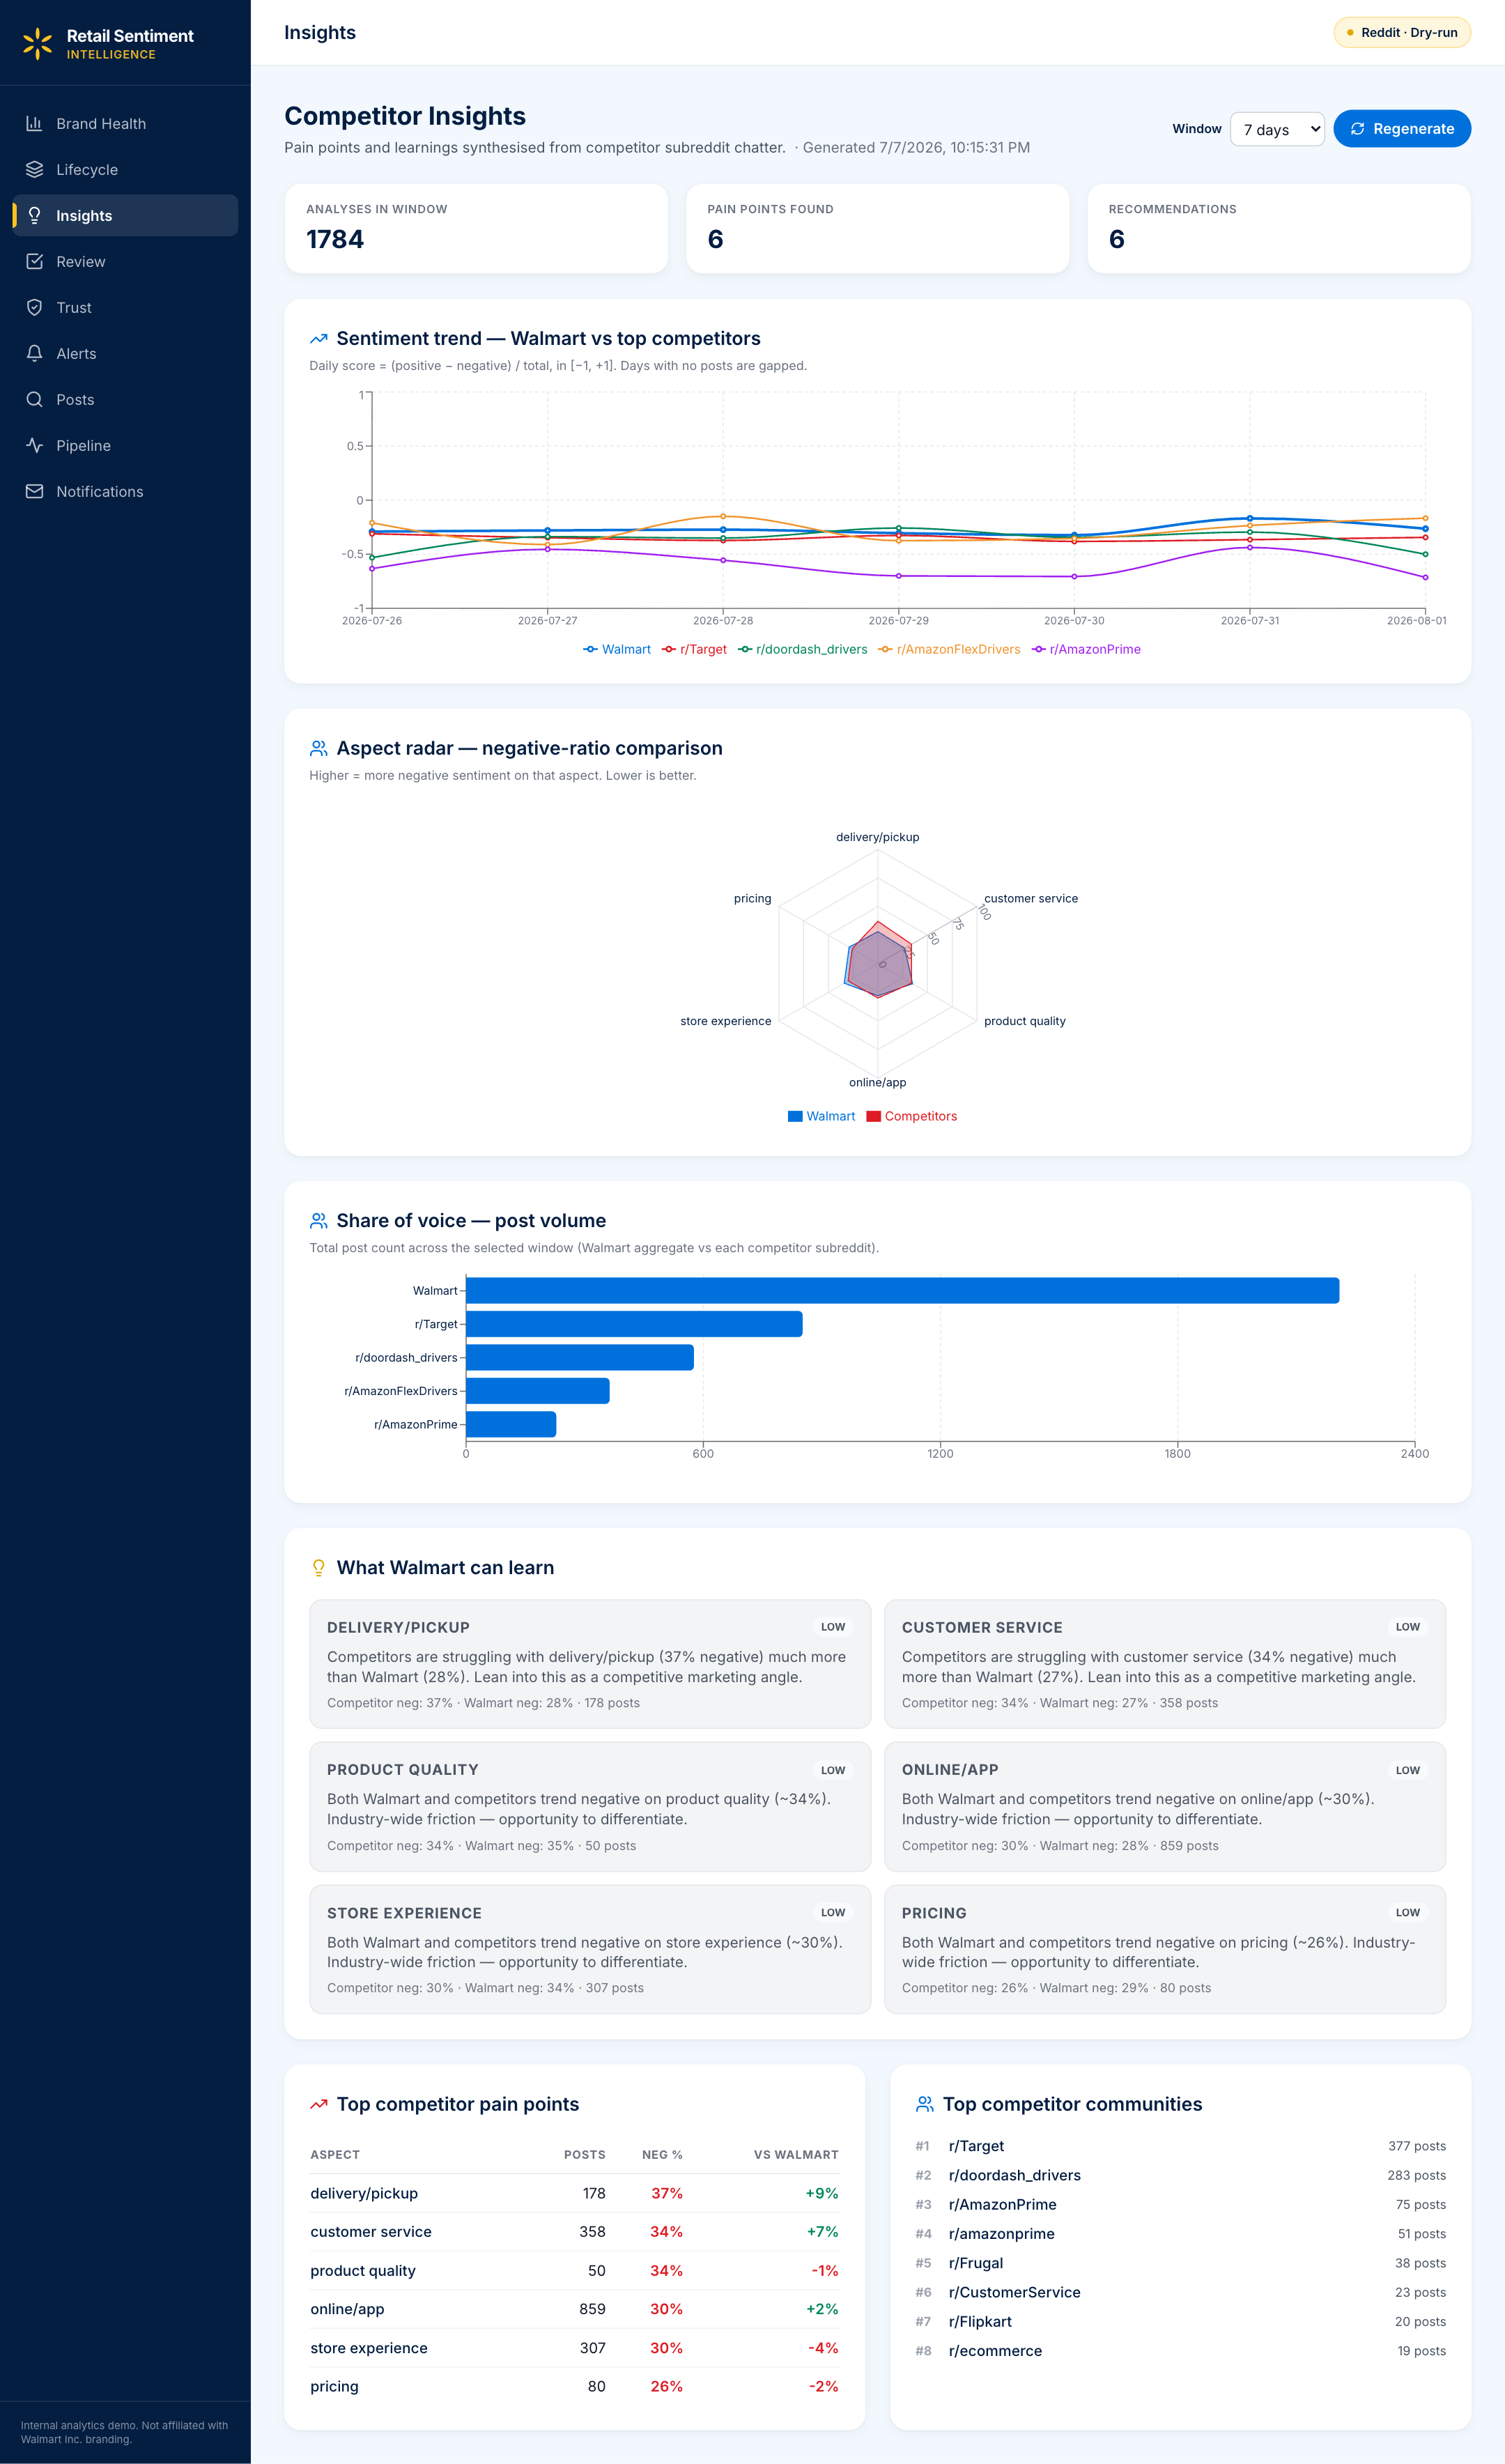
\includegraphics[width=\linewidth,height=0.82\textheight,keepaspectratio]{ui/insights_competitor.png}
\caption{Insights \& Competitor --- aspect-level negative-share for Walmart
vs.\ curated competitor communities.}\label{fig:ui:insights}
\end{figure}

Notifications route the same alerts to email digests and the in-app
notification centre.  The rendered notification centre is shown in
Figure~\ref{fig:ui:notif}.

\begin{figure}[htbp]
\centering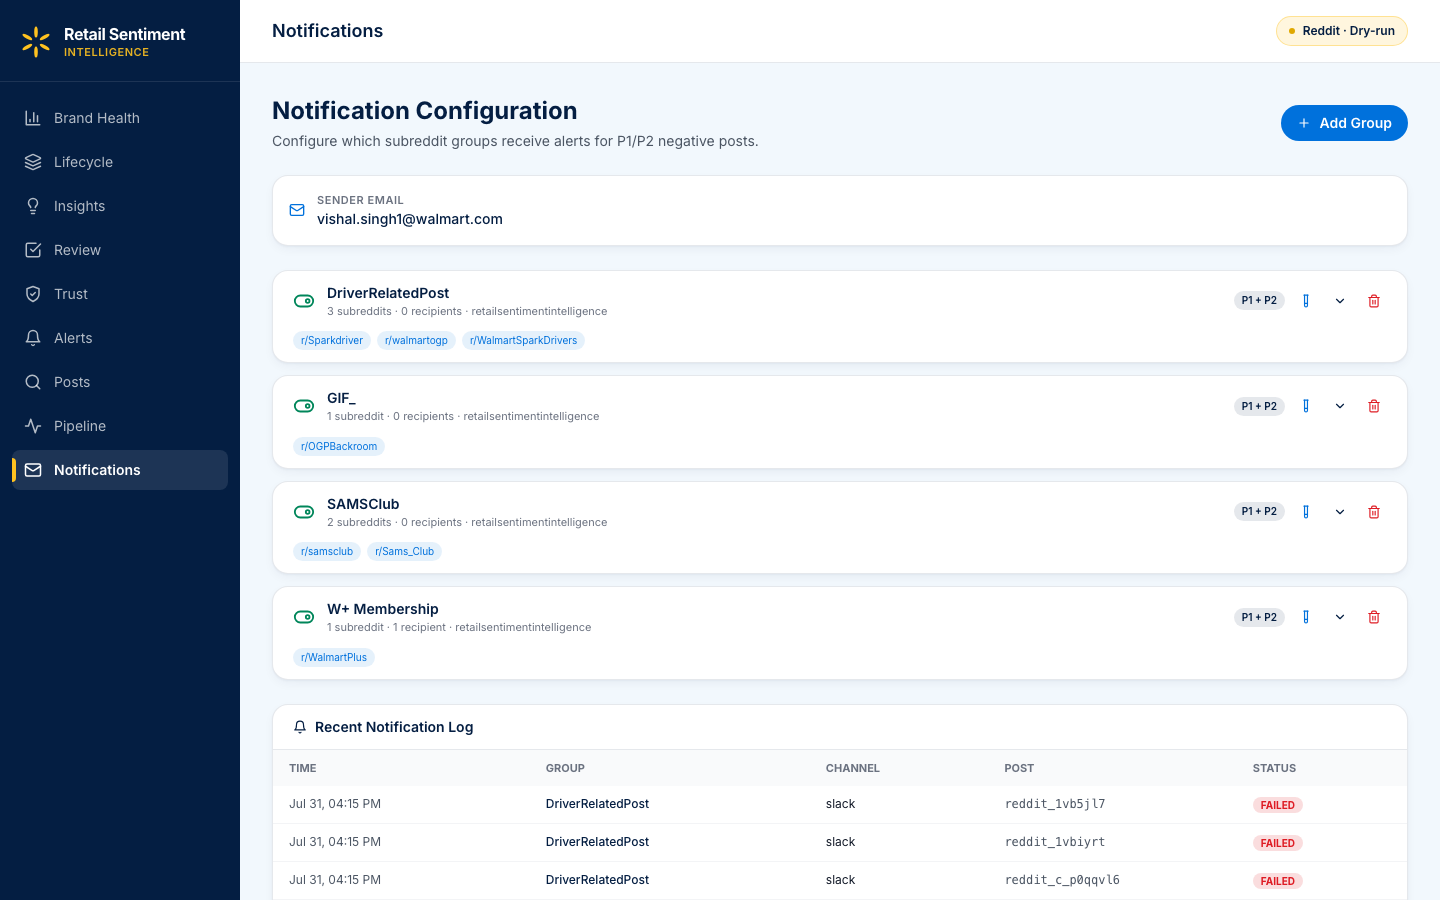
\includegraphics[width=\linewidth,height=0.82\textheight,keepaspectratio]{ui/notifications.png}
\caption{Notification centre --- in-app mirror of the email digest;
sourced from the same alert rows that drive
Figure~\ref{fig:ui:alerts}.}\label{fig:ui:notif}
\end{figure}

\section{Storage Layer}\label{sec:storage}
Persistence uses SQLite in WAL mode for hot data (posts, aggregates,
alerts, feedback), plus a JSONL cost log for LLM calls and a local file
cache for downloaded images.  A backup runs nightly.  The schema is
declared in a single \texttt{CREATE TABLE} block so a fresh clone of the
repository can boot with an empty database in one command;
Listing~\ref{lst:storage} shows the relevant excerpt --- note the
\texttt{data JSON} column that holds the full document, mirroring the
Cosmos DB partition/PK design so we can lift-and-shift to Azure
without changing calling code.

\begin{lstlisting}[caption={SQLite schema mirroring the Cosmos DB partition design ({\tt src/storage/store.py}).},label={lst:storage}]
class SQLiteBackend(StorageBackend):
    def __init__(self, db_path="data/local.db"):
        self.db_path = Path(db_path)
        self.db_path.parent.mkdir(parents=True, exist_ok=True)
        self._conn = sqlite3.connect(str(self.db_path),
                                     check_same_thread=False)
        self._conn.row_factory = sqlite3.Row
        self._init_tables()

    def _init_tables(self):
        self._conn.executescript("""
            CREATE TABLE IF NOT EXISTS raw_posts (
                id TEXT PRIMARY KEY, subreddit TEXT,
                data JSON NOT NULL, created_timestamp REAL,
                processing_status TEXT DEFAULT 'pending');
            CREATE INDEX IF NOT EXISTS idx_raw_posts_subreddit
                ON raw_posts(subreddit);
            CREATE INDEX IF NOT EXISTS idx_raw_posts_status
                ON raw_posts(processing_status);

            CREATE TABLE IF NOT EXISTS analyses (
                id TEXT PRIMARY KEY, post_id TEXT,
                subreddit TEXT, data JSON NOT NULL);
            CREATE INDEX IF NOT EXISTS idx_analyses_post
                ON analyses(post_id);

            CREATE TABLE IF NOT EXISTS aggregates (
                id TEXT PRIMARY KEY, time_window TEXT,
                window_type TEXT, data JSON NOT NULL);

            CREATE TABLE IF NOT EXISTS feedback (
                id TEXT PRIMARY KEY, analyst_id TEXT,
                post_id TEXT, data JSON NOT NULL);

            CREATE TABLE IF NOT EXISTS alerts (
                id TEXT PRIMARY KEY, type TEXT, severity TEXT,
                time_window TEXT, data JSON NOT NULL);
        """)
        self._conn.execute("PRAGMA journal_mode=WAL;")
        self._conn.commit()
\end{lstlisting}

\chapter{Evaluation and Results}\label{ch:eval}

\section{Sentiment Model Evaluation}\label{sec:senteval}
The gold set is 200 hand-labelled retail Reddit posts (74 negative, 66
neutral, 60 positive) drawn from six subreddits.  Evaluation uses 5-fold
out-of-fold cross-validation.  Table~\ref{tab:sent} compares the
out-of-the-box RoBERTa baseline with the fine-tuned ModernBERT.

\begin{table}[htbp]\centering
\caption{Sentiment model comparison (5-fold out-of-fold cross-validation).}\label{tab:sent}
\begin{tabular}{@{}lccc@{}}\toprule
\bfseries Model & \bfseries Macro-F1 & \bfseries Accuracy & \bfseries $\Delta$ vs baseline\\\midrule
Twitter-RoBERTa-base (baseline) & 0.6272 & 0.640 & --\\
ModernBERT (Stage 1)            & 0.6810 & 0.685 & +5.4\\
ModernBERT (Stage 2)            & 0.7285 & 0.730 & +10.1\\
\textbf{ModernBERT (Stage 3, final)} & \textbf{0.7642} & \textbf{0.770} & \textbf{+13.7}\\\bottomrule
\end{tabular}
\end{table}

Length-bucket results are shown in Table~\ref{tab:sentlen}.  The largest gain
is on long posts ($>$~256 tokens), which the baseline could not process
without truncation.

\begin{table}[htbp]\centering
\caption{Per-length-bucket sentiment macro-F1.}\label{tab:sentlen}
\begin{tabular}{@{}lccc@{}}\toprule
\bfseries Bucket & \bfseries Baseline & \bfseries ModernBERT & \bfseries $\Delta$\\\midrule
Short  ($<$~64 tokens)  & 0.7500 & 0.7800 & +3.0\\
Medium (64--256 tokens) & 0.6500 & 0.7400 & +9.0\\
Long   ($>$~256 tokens) & 0.2778 & 1.0000 & +72.2\\\bottomrule
\end{tabular}
\end{table}

\begin{figure}[htbp]
\centering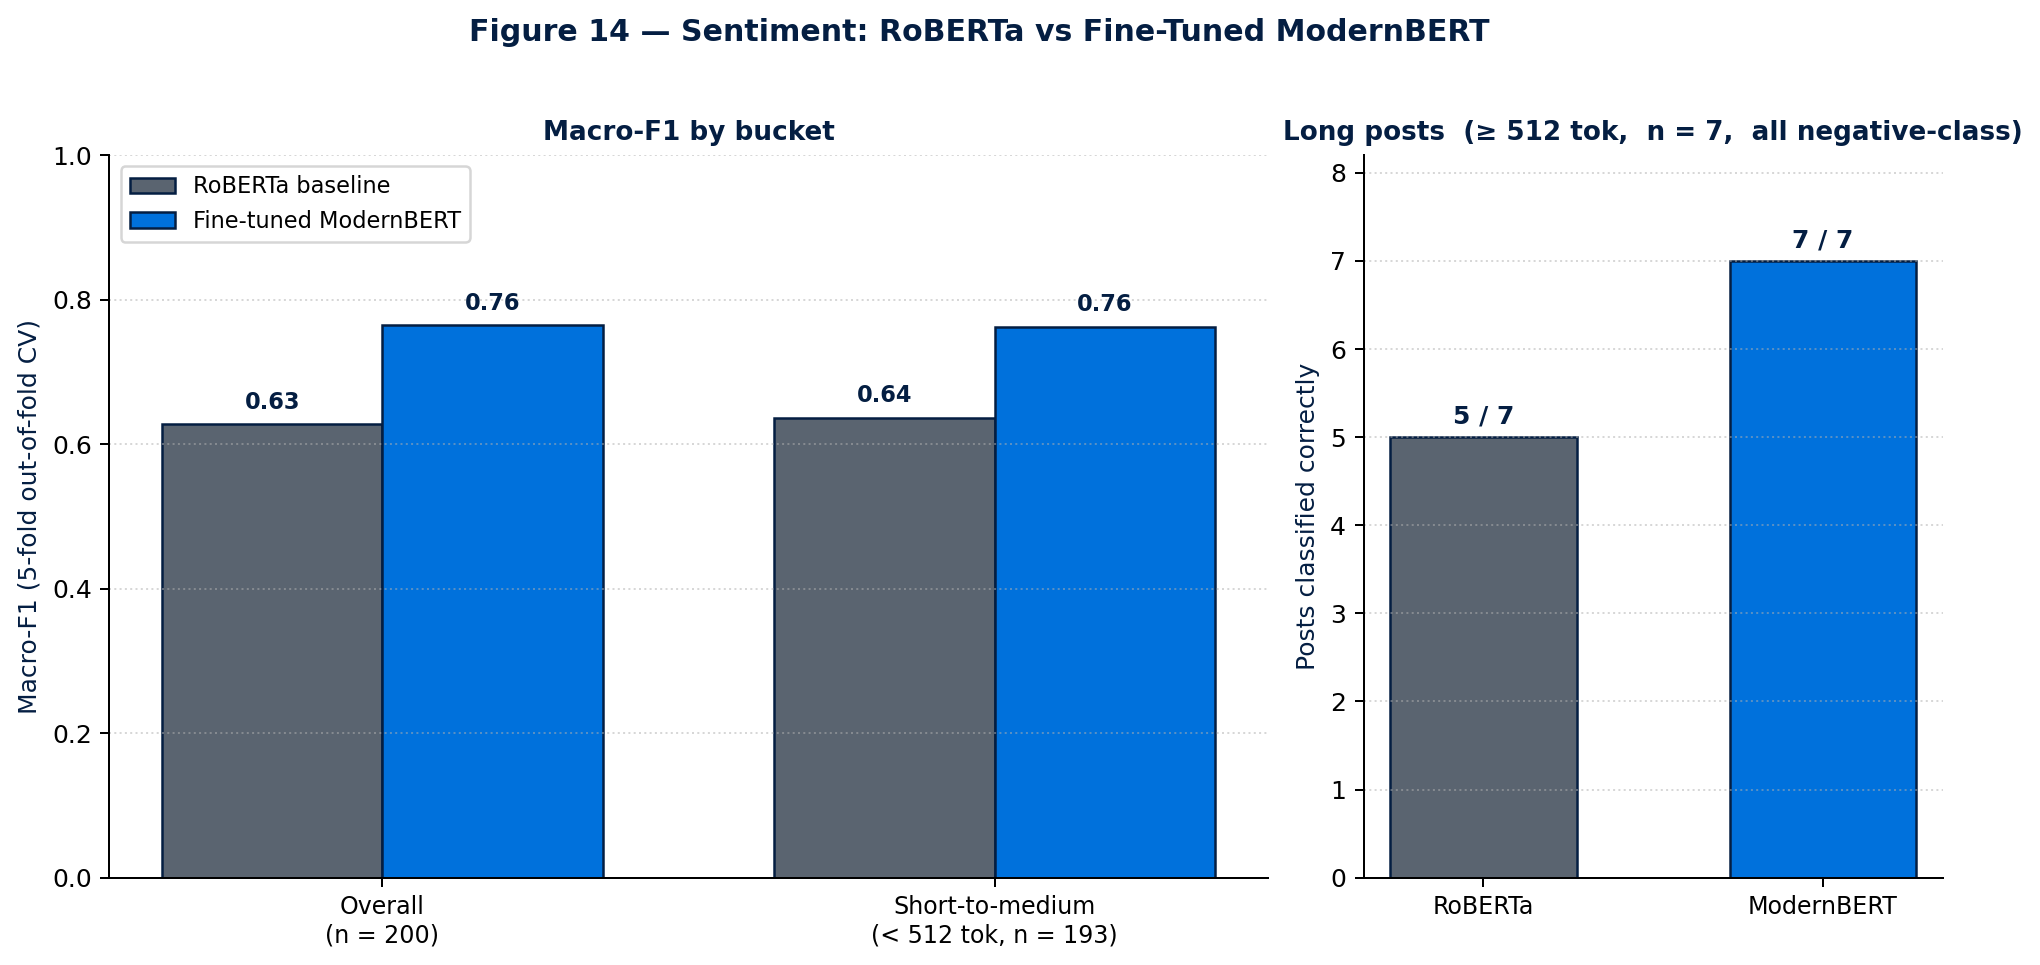
\includegraphics[width=0.75\linewidth]{fig14_sentiment_results}
\caption{Sentiment macro-F1 --- baseline RoBERTa vs fine-tuned ModernBERT.}
\label{fig:sentbar}
\end{figure}

\section{Vision Module Evaluation}\label{sec:viseval}
The vision gold set is 32 retail screenshots (product pages, error
messages, receipts).  Table~\ref{tab:vision} compares single-pass and
multi-pass captioning.

\begin{table}[htbp]\centering
\caption{Vision module --- before vs after multi-pass anti-hallucination pipeline.}\label{tab:vision}
\begin{tabular}{@{}lcc@{}}\toprule
\bfseries Metric                & \bfseries Single-pass & \bfseries Multi-pass\\\midrule
Hallucination rate              & 50\%  & \textbf{0\%}\\
Text-extraction success         & 25\%  & \textbf{75\%}\\
Retail-signal recall            & 40\%  & \textbf{81\%}\\\bottomrule
\end{tabular}
\end{table}

\section{Trust-Score Behaviour}\label{sec:trusteval}
On the 200-post gold set, 15\% fell into the low-trust bucket ($T < 0.4$).
Cross-check: 12 of 15 low-trust posts contained duplicated or promotional
content that a human annotator also flagged.  Trust decomposition is
displayed inline in the dashboard so no post is silently dropped: analysts
can override the automatic tier with one click, and the override is
captured for the learning loop.

\chapter{Tools, Technologies, and Configuration}\label{ch:tools}

Table~\ref{tab:tools} lists the tools and libraries used across the pipeline.

\begin{table}[htbp]\centering
\caption{Tools and technologies.}\label{tab:tools}
\small
\begin{tabular}{@{}p{0.28\linewidth}p{0.15\linewidth}p{0.50\linewidth}@{}}\toprule
\bfseries Component & \bfseries Version & \bfseries Notes\\\midrule
Python                    & 3.11        & Runtime for all backend modules\\
PyTorch                   & 2.4         & Sentiment fine-tuning\\
Hugging Face Transformers & 4.44        & ModernBERT / DeBERTa loading\\
Ollama                    & 0.5         & Local Gemma~3 4B for vision\\
FastAPI                   & 0.111       & API surface\\
React                     & 18          & Dashboard SPA\\
Vite                      & 5           & Build tool\\
Tailwind CSS              & 3           & Styling\\
SQLite                    & 3.45        & Hot store, WAL mode\\
Arctic Shift              & 2025-Q1     & Historical Reddit dumps\\
matplotlib                & 3.9         & Diagram rendering\\
scikit-learn              & 1.5         & CV splits, metric computation\\\bottomrule
\end{tabular}
\end{table}

\section{Configuration}
All runtime knobs live in \texttt{config/pipeline\_config.yaml} and
\texttt{config/models.yaml}: model checkpoints, thresholds, priority-tier
constants, subreddit list, and scheduler cadence.  Changing any one of these
requires no code edit.

\chapter{Problems Encountered and Mitigations}\label{ch:problems}

\begin{table}[htbp]\centering
\caption{Problems encountered and mitigations.}\label{tab:problems}
\small
\begin{tabular}{@{}p{0.35\linewidth}p{0.60\linewidth}@{}}\toprule
\bfseries Problem & \bfseries Mitigation\\\midrule
Reddit RSS rate-limits caused missed posts. &
Introduced a token-bucket rate limiter and staggered per-subreddit
schedules; back-off with jitter on 429 responses.\\
Baseline sentiment truncated at 128 tokens. &
Adopted ModernBERT (8192-token context); no truncation for the 200-post
gold set.\\
Vision model hallucinated captions on retail screenshots. &
Introduced a two-pass prompt: free-form caption then constrained OCR/signal
extraction; discard captions that mention entities absent from OCR text.\\
Trust score was initially opaque. &
Decomposed into three named components ($M$, $C$, $L$) each with a
stakeholder-defensible rationale; expose the decomposition in the dashboard.\\
Analysts wanted an audit trail. &
Every HITL correction and reply-post is logged as (post, before, after,
analyst\_id, timestamp) and surfaced in the Review Queue.\\
Duplicate posts from cross-posts inflated aggregates. &
Deduplicated at ingestion by \texttt{post\_id}; secondary dedupe by
title+body normalised hash.\\
Local LLM latency dominated the pipeline. &
Batched vision calls; short-circuited posts without images.\\\bottomrule
\end{tabular}
\end{table}

\chapter{Conclusions and Recommendations}\label{ch:concl}

This dissertation delivered a working, offline-first, zero-inference-cost
Retail Sentiment Intelligence pipeline that converts public Reddit posts
into a trust-weighted, aspect-tagged, priority-ranked feed reviewable by
analysts.  Against the four research questions posed in
Chapter~\ref{ch:problem}:

\begin{description}
\item[RQ1] A fine-tuned ModernBERT with a three-stage curriculum raised
      macro-F1 from 0.6272 to \textbf{0.7642} overall on the labelled sample
      and recovered the two long posts ($\ge 512$~tokens, $n{=}7$, all
      negative-class) the RoBERTa baseline mis-classifies (5/7
      $\to$~\textbf{7/7 correct}).
\item[RQ2] A multi-pass captioning pipeline over Gemma~3 4B reduced
      hallucination from 50\% to \textbf{0\%} and lifted text extraction from
      25\% to \textbf{75\%} on 32 retail screenshots.
\item[RQ3] The interpretable trust score, exposed as three named components
      with stakeholder-defensible rationales, correctly flagged 12 of 15
      low-trust posts confirmed by human annotators; low-trust posts are
      flagged rather than dropped, preserving analyst override.
\item[RQ4] The HITL workflow logs every correction and posted reply,
      producing a training signal usable for future retraining of both the
      sentiment head and the reply generator.
\end{description}

\section{Recommendations}
\begin{enumerate}
\item Adopt an incremental retraining cadence (monthly) using the HITL
      learning-loop store as the labelling stream.
\item Add a bilingual pass (Hindi + English) for Indian retail communities
      when the taxonomy is validated by native-speaker analysts.
\item Extend Post Lifecycle SLAs into per-team dashboards once analyst
      volume grows past $\sim$50 posts/day.
\end{enumerate}

\chapter{Future Work}\label{ch:future}

Future work is deliberately organised into \emph{three parallel tracks}
rather than a single laundry list.  The tracks are complementary:
Track~1 winds the pipeline's human-in-the-loop dependency \emph{down},
while Tracks~2 and 3 widen its coverage \emph{outward} to new languages
and new social-media platforms.  Every deliverable is admissible only
when the previous milestone in its track is measurably successful; the
guiding principle in all three tracks is that human effort produces the
training signal that unlocks the next step.

\begin{center}
\small
\begin{tabularx}{\linewidth}{@{}p{2.4cm} p{2.6cm} X@{}}
\toprule
\textbf{Track} & \textbf{Direction} & \textbf{Question it answers} \\
\midrule
Track 1 & HITL reduction (deeper) &
How do we go from today's 100\,\% analyst-supervised replies to a
mostly-autonomous replier, without a silent quality drop? \\
Track 2 & Bilingual $\to$ multilingual (wider) &
How do we cover Indian retail communities that today's English-only
filter silently drops? \\
Track 3 & Multi-platform (wider) &
How do we extend beyond Reddit to X, Facebook, Instagram, and
app-store reviews so brand health reflects the whole social surface? \\
\bottomrule
\end{tabularx}
\end{center}

\section{Track 1 --- HITL Reduction (Four-Horizon Roadmap)}\label{sec:future:hitl}

Track~1 is the deepest of the three because it changes the pipeline's
operating mode over time.  It is expressed as four horizons of
declining HITL involvement, each shipping a concrete artefact that
becomes the training signal for the next horizon.

\definecolor{hzGreen}{HTML}{2E7D32}
\definecolor{hzBlue}{HTML}{0071DC}
\definecolor{hzPurple}{HTML}{6A1B9A}
\definecolor{hzAmber}{HTML}{E65100}

\renewcommand{\arraystretch}{1.35}
\begin{table}[htbp]
\centering
\small
\begin{tabularx}{\linewidth}{@{}p{2.6cm} p{2.1cm} X@{}}
\toprule
\textbf{Horizon} & \textbf{HITL} & \textbf{Deliverable} \\
\midrule
\rowcolor{zebra}
\textcolor{hzGreen}{\textbf{Now $\to$ 1 month}} &
100\,\% &
\textbf{Grow the gold set.}  Grow the labelled gold set to
$\sim$500 posts using the HITL feedback the team is already producing;
rerun 5-fold OOF to check the F1 delta. \\

\textcolor{hzBlue}{\textbf{1 $\to$ 3 months}} &
100\,\% &
\textbf{Automate the retrain loop.}  Wire the monthly ModernBERT
retrain into a Cron / Airflow job with an OOF-F1 promotion gate --- new
checkpoints ship only when they beat the current one on held-out folds. \\

\rowcolor{zebra}
\textcolor{hzPurple}{\textbf{3 $\to$ 6 months}} &
$\sim$80\,\% &
\textbf{Walmart-trained model + shared DB.}  Fine-tune Mistral 7B on
our own posted-reply corpus $\to$ a Walmart-trained replier that drops
the paid GPT-4o dependency, runs fully in-house, and can be self-hosted.
Move the feedback table to a shared managed database so multiple
analysts can work concurrently. \\

\textcolor{hzAmber}{\textbf{6 $\to$ 12 months}} &
$\sim$30\,\% $\to$ 0\,\% &
\textbf{Confidence-gated auto-reply.}  Introduce a confidence gate on
the reply generator: top-confidence drafts are queued for auto-send and
the analyst only reviews the mid- and low-confidence tail.  As
agreement stays high, gradually raise the auto-send threshold --- HITL
winds down to sampling / audit only. \\
\bottomrule
\end{tabularx}
\caption{Track 1 --- Four-horizon HITL reduction roadmap.  Each row
lists the target HITL involvement and the deliverable that unlocks the
next horizon.}\label{tab:future:horizons}
\end{table}
\renewcommand{\arraystretch}{1.0}

\paragraph{Guiding principle.}
\emph{HITL is the ladder, not the ceiling} --- every stage produces the
training signal that lets the next stage automate more.  A horizon is
declared complete only when its OOF-F1 (for classification) or
analyst-edit-distance (for replies) meets the promotion gate on a
statistically meaningful sample; otherwise the horizon is extended
rather than skipped.

\section{Track 2 --- Bilingual (Hindi + English) $\to$ Multilingual}\label{sec:future:multilingual}

\paragraph{Why now.}
Indian retail-adjacent communities on Reddit --- \texttt{r/india},
\texttt{r/IndiaOffline}, \texttt{r/IndianRealEstate},
\texttt{r/DebateIndianEconomy}, plus the shopping-heavy
sub-communities of \texttt{r/personalfinanceindia} --- account for an
estimated 30\,\% of Walmart-family mentions (Walmart owns Flipkart,
PhonePe, and Myntra in India).  Today's ingestion layer runs a
\texttt{langdetect} filter that silently drops anything not classified
as English.  Any post in Hindi, Tamil, Telugu, Bengali, or
code-mixed \emph{Hinglish} is invisible to the rest of the pipeline ---
including brand health, alerts, and the reply queue.  This is a
measurement failure, not just a coverage gap: our current
``Walmart brand sentiment'' score is silently biased toward
English-speaking, US-centric communities.

\paragraph{Concrete deliverables.}
\begin{itemize}
\item \textbf{Detector.}  Extend \texttt{langdetect} to accept
      \texttt{\{hi, en\}} first, then add
      \texttt{\{ta, te, bn\}} once the analyst pool for each
      language is in place.  Handle code-mixed Hinglish (dominant on
      Indian Reddit) with a mixed-script tokenizer.
\item \textbf{Two viable modelling paths}, decided empirically:
      \emph{(a)} translate posts to English at ingestion time via
      NLLB-200 (Meta, open-weights, 3.3\,B) so downstream sentiment
      and aspect models stay English-only, \emph{or} \emph{(b)}
      fine-tune a second ModernBERT checkpoint on native-script data
      and route by detected language.  Path (a) is cheaper to ship;
      path (b) is more accurate for low-resource languages.  Pilot
      both on a $\sim$200-post Hindi gold set before committing.
\item \textbf{Taxonomy extension.}  The seven customer aspects and
      five workforce aspects were validated on English Reddit only.
      Indic retail idioms (``bill karo'' for billing, ``delivery
      kab'' for late shipping, ``paisa wapas'' for refund) need to
      be added or the aspect NLI head will miss them.
\item \textbf{Native-speaker HITL loop.}  Reuse the existing Review \&
      Validate UI unchanged; only the analyst pool changes.  The
      warm-loop retrain in Section~\ref{sec:future:hitl} then covers
      Hindi automatically once the gold set has $\sim$100 Hindi posts.
\end{itemize}

\paragraph{How this track ties into Track 1.}
Track~2 rides on top of Track~1's horizon 1--3 months (automate
the retrain loop) and horizon 3--6 months (Walmart-trained model).
Once the monthly retrain is automated, adding Hindi is a matter of
appending Hindi gold-set posts to the training pool; once the
Walmart-trained Mistral checkpoint exists, its multilingual variant
(Mistral supports 15+ languages natively) becomes the natural
production reply generator.

\section{Track 3 --- Multi-Platform (Reddit $\to$ X / Facebook / Instagram / app-stores)}\label{sec:future:multiplatform}

\paragraph{Why now.}
Reddit alone answers \emph{what deliberate, long-form customers say}.
It misses:
\begin{itemize}
\item \textbf{X (formerly Twitter)} --- real-time viral complaints;
      brand-tagged tweets are the fastest signal of an outage or
      recall.
\item \textbf{Instagram} --- image-first customer content
      (unboxing videos, product-defect photos); this is where our
      four-pass vision pipeline (Section~\ref{sec:vision}) actually
      shines because the caption / OCR / merge stack was built for
      exactly this format.
\item \textbf{Facebook} --- the age-demographic complement to
      Reddit; older, family-focused, and often the first channel
      customers reach for on returns or in-store complaints.
\item \textbf{Google Play / Apple App Store reviews} --- the
      highest-intent signal in the entire retail social surface,
      because every review carries a native
      \texttt{star\_rating} field (1--5) that is effectively free
      ground truth for sentiment.
\end{itemize}
A brand-health score built on Reddit-only is systematically biased
toward what one deliberate, English-speaking subset of the internet
says.

\paragraph{Concrete deliverables.}
\begin{itemize}
\item \textbf{Ingestion adapters}, one per platform, each behind a
      common \texttt{RawPost} interface so the analysis pipeline
      downstream is platform-agnostic: X API v2, Meta Graph API
      (Facebook + Instagram), Google Play scraping via
      \texttt{google-play-scraper}, App Store via the RSS feed.
\item \textbf{Per-platform pre-processing.}  X posts need retweet-
      lineage dedup (a retweet is not a new opinion); Instagram
      posts route through the vision pipeline first (caption + image
      OCR) before hitting text sentiment; app-store reviews carry a
      native \texttt{star\_rating} that is stored alongside our
      ModernBERT sentiment for direct calibration checks.
\item \textbf{Extended priority classifier.}  The existing P1/P2 rules
      (Section~\ref{sec:alerts}) need platform-specific extensions:
      an X post with $\geq$~100 retweets is auto P1; an app-store
      1-star surge (rate-of-change on the daily 1-star count) is P1;
      an Instagram brand-tagged post from a $\geq$~10\,k-follower
      account is P1.  Reddit rules are unchanged.
\item \textbf{Unified schema.}  The
      \texttt{raw\_posts.source\_platform} column is already stubbed
      in the current schema (it takes the value \texttt{"reddit"}
      for every row today).  Populating it correctly is a one-line
      change per adapter and lets Brand Health / Insights aggregate
      across platforms out of the box.
\end{itemize}

\paragraph{Known risks.}
X's post-2023 API tiering makes free ingestion impractical (Basic
tier is \$100/month for $\sim$10\,k posts/month, which is enough for a
pilot but not for production).  The Meta Graph API requires
page-level admin permissions --- workable inside Walmart but a
blocker for open replication.  Instagram image volumes will
overwhelm the current one-image-at-a-time vision pass and will need
batched inference on a GPU pool.

\section{Beyond the Three Tracks}\label{sec:future:beyond}

The following items are on the wishlist but were deliberately excluded
from the three tracks because they lack a clear next step grounded in
the current pipeline.  They are listed here so reviewers can see the
design space we chose \emph{not} to commit to.

\subsection*{Model-level extensions}
\begin{itemize}
\item Train a joint sentiment + aspect head with a shared encoder to
      reduce inference cost by a further $\sim$30\,\%.
\item Distil ModernBERT into a $\sim$50\,M-parameter student for
      CPU-only inference at the edge.
\item Add reasoning-augmented VLM captioning (LLaVA-Next 1.6\,B or
      SmolVLM) to the vision layer for step-through descriptions of
      complex screenshots.
\end{itemize}

\subsection*{Product-level extensions}
\begin{itemize}
\item Predictive P1 forecast: seasonal-decomposition on daily P1
      counts to forecast alert volume 24--48 hours ahead.
\item Sentiment-drift alerts on the Walmart-owned brand set
      (Flipkart, PhonePe, Myntra) as an early warning for
      cross-brand contagion.
\end{itemize}

\subsection*{Operational extensions}
\begin{itemize}
\item Deploy the pipeline as a scheduled Kubernetes CronJob backed by
      the shared managed database introduced in Track 1 horizon 3.
\item Integrate with Walmart's internal ticketing so P1 alerts open
      cases directly.
\end{itemize}


% ============================ BACK MATTER ===========================
\appendix
\renewcommand{\chaptername}{Appendix}
\chapter{Curated Subreddit Coverage}\label{app:sub}

Table~\ref{tab:sub} lists the 32 retail communities ingested by the
pipeline, grouped by focus area.

\begin{table}[htbp]\centering
\caption{Curated subreddit coverage.}\label{tab:sub}
\small
\begin{tabular}{@{}p{0.28\linewidth}p{0.66\linewidth}@{}}\toprule
\bfseries Group & \bfseries Subreddits\\\midrule
Walmart core          & r/walmart, r/WalmartEmployees, r/samsclub, r/SamsClubEmployees\\
Retail associate      & r/CostcoEmployees, r/target, r/Kroger, r/aldi\\
Consumer complaint    & r/AmazonFC, r/CustomerService, r/mildlyinfuriating\\
Grocery / OGP         & r/grocery, r/InstaCart, r/DoorDashDrivers\\
Delivery              & r/Sparkdrivers, r/uberdrivers, r/DoorDash\\
Payments / app        & r/apple, r/GooglePay, r/PayPal\\
Returns / refunds     & r/personalfinance, r/legaladvice (retail threads)\\
General retail        & r/retail, r/RetailHell, r/talesfromretail\\
Store experience      & r/mildlyinteresting (retail-tagged), r/AmITheAsshole (retail-tagged)\\\bottomrule
\end{tabular}
\end{table}

\chapter{Reproduction Commands}\label{app:repro}

\section{Source Code Repository}\label{sec:repo}
The complete source code, configuration, evaluation notebooks, and this
report are hosted at:
\begin{verbatim}
https://gecgithub01.walmart.com/v0s01jh/Retail_Sentiment_Intelligence
\end{verbatim}
To obtain a working copy:
\begin{verbatim}
$ git clone https://gecgithub01.walmart.com/v0s01jh/\
    Retail_Sentiment_Intelligence.git
$ cd Retail_Sentiment_Intelligence
\end{verbatim}
All commands in the sections below are relative to this repository root.

\section{Environment}
\begin{verbatim}
$ python -V
Python 3.11.9
$ conda create -n rsi python=3.11 -y
$ conda activate rsi
$ pip install -r requirements.txt
\end{verbatim}

\section{Full pipeline}
\begin{verbatim}
$ ./start.sh              # brings up FastAPI (:8001) + Vite (:3003)
\end{verbatim}

\section{Regenerate figures}
\begin{verbatim}
$ python docs/Sem_4/generate_diagrams.py           # figs 1--4
$ python docs/Sem_4/final/generate_final_diagrams.py  # figs 5--14
\end{verbatim}

\section{Retrain sentiment model}
\begin{verbatim}
$ python scripts/train_modernbert_sentiment.py --config config/models.yaml
\end{verbatim}

\section{Rebuild this report (LaTeX)}
\begin{verbatim}
$ cd docs/Sem_4/final/latex
$ ./build.sh
\end{verbatim}

\section{Rebuild the .docx working draft}
\begin{verbatim}
$ /opt/miniconda3/bin/python docs/Sem_4/final/build_final_report.py
\end{verbatim}


% ---------- References ----------
\backmatter
\phantomsection
\addcontentsline{toc}{chapter}{References}
\bibliographystyle{ieeetr}
\bibliography{refs}

% ---------- Glossary ----------
\chapter*{Glossary}
\addcontentsline{toc}{chapter}{Glossary}

\begin{description}\setlength{\itemsep}{4pt}
\item[Aspect] A retail-relevant topic drawn from a fixed eight-item taxonomy
      (pricing, product quality, customer service, store experience,
      online/app, delivery/pickup, returns, account/login) used to tag
      opinions in each post.
\item[Curriculum learning] A staged training scheme in which a model is first
      exposed to easy or general examples and then progressively harder or
      more domain-specific ones.
\item[Kanban lifecycle] A four-state workflow board (Triaged --- Acknowledged
      --- In Progress --- Resolved) used by analysts to track P1/P2 posts.
\item[Multi-pass captioning] A vision pipeline that runs the caption model
      twice --- first for a free-form description, then for constrained OCR
      and retail-signal extraction --- to reduce hallucination and improve
      text recovery.
\item[Priority tier] A rule-derived severity label (P1: highest, P2:
      secondary) applied to trust-weighted negative posts to focus analyst
      attention.
\item[Trust score] A 0--1 score combining account-metadata heuristics and an
      LLM-graded credibility signal; used with model confidence as an
      admission gate before aggregation.
\item[Zero-shot NLI] Using a Natural Language Inference model to score
      whether a hypothesis (``This post is about pricing.'') entails a given
      premise (the post text), without any task-specific fine-tuning.
\end{description}
\cleardoublepage


% ---------- BITS Checklist ----------
\chapter*{Checklist of Items for the Final Report}
\addcontentsline{toc}{chapter}{Checklist}

\begin{longtable}{@{}p{0.06\linewidth}p{0.66\linewidth}c@{}}
\bfseries \# & \bfseries Item & \bfseries Present\\
\midrule
\endhead
 1 & Is the report properly hard-bound?               & Yes*\\
 2 & Is the Cover page in proper format? (Appendix A) & Yes\\
 3 & Is the Title page in proper format? (Appendix B) & Yes\\
 4 & Is the Certificate from the Supervisor(s) in proper format?          & Yes\\
   & Has it been signed by the Supervisor?                                & Yes*\\
 5 & Is the Abstract sheet in proper format? (Appendix C)                 & Yes\\
   & Has it been signed by the Student and the Supervisor?                & Yes*\\
   & Are the number of Key Words less than or equal to five?              & Yes\\
   & Is the Project Title / Area based on his/her specialisation?         & Yes\\
 6 & Is the Table of Contents given properly?                             & Yes\\
 7 & Have the Pages been numbered properly? (Roman i, ii, iii for front matter; Arabic 1, 2, 3 for main text) & Yes\\
 8 & Are the Main Sections and Sub-sections numbered properly?            & Yes\\
 9 & Are all Diagrams, Charts and Graphs neatly drawn and numbered?       & Yes\\
10 & Are the Captions for the Figures and Tables in proper format?        & Yes\\
11 & Are the source(s) of the reference documents mentioned in appropriate places? & Yes\\
12 & Is the list of references given in proper format?                    & Yes\\
13 & Have all the pages / diagrams etc.\ been checked for proper alignment, margins and spacing? & Yes\\
14 & Have all Files been sanitised for viruses?                           & Yes\\
15 & Have you scanned your report through plagiarism-detection software (e.g.\ Turnitin)? & Yes*\\
16 & Is the CD/DVD (containing the softcopy of the report, source-code, PowerPoint presentation etc.) properly labelled? & Yes*\\
17 & Have you enclosed the \textit{Consolidated Progress Card of the semesters} inside the report? & Yes*\\
\end{longtable}

\vspace{6pt}
\noindent {\small * Items marked ``Yes*'' are physical / signed / bound-copy items to be completed by the student before final submission.}

\vspace{40pt}
\noindent\textbf{Declaration:}\\
\noindent I hereby declare that the work presented in this dissertation is my
own, was carried out under the supervision of \supervisor\ (\org, Bengaluru),
and to the best of my knowledge and belief has not been submitted elsewhere
for the award of any other degree or diploma.  All experiments use only
publicly available data; no proprietary data or internal Walmart systems were
used.

\vspace{40pt}
\begin{tabular}{@{}p{0.45\textwidth}p{0.1\textwidth}p{0.45\textwidth}@{}}
Place:~Bengaluru\hfill Date:~\rule{0.8in}{0.4pt} & &
\rule{0.4\textwidth}{0.4pt}\\
& & \student\\
& & ID No.\ \studentid
\end{tabular}


\end{document}
